%% LyX 2.2.1 created this file.  For more info, see http://www.lyx.org/.
%% Do not edit unless you really know what you are doing.
\documentclass[english]{aghdpl}
\usepackage[T1]{fontenc}
\usepackage[utf8]{inputenc}
\setcounter{secnumdepth}{3}
\setcounter{tocdepth}{3}
\usepackage{babel}
\usepackage{verbatim}
\usepackage{float}
\usepackage{mathtools}
\usepackage{amsmath}
\usepackage{graphicx}
\usepackage[unicode=true,pdfusetitle,
 bookmarks=true,bookmarksnumbered=true,bookmarksopen=true,bookmarksopenlevel=3,
 breaklinks=false,pdfborder={0 0 1},backref=false,colorlinks=false]
 {hyperref}
\usepackage{breakurl}

\makeatletter

%%%%%%%%%%%%%%%%%%%%%%%%%%%%%% LyX specific LaTeX commands.

\newcommand*\LyXZeroWidthSpace{\hspace{0pt}}
%% Because html converters don't know tabularnewline
\providecommand{\tabularnewline}{\\}

%%%%%%%%%%%%%%%%%%%%%%%%%%%%%% User specified LaTeX commands.
\usepackage{babel}
\usepackage{polski}





\usepackage{amsfonts}
\usepackage{amsthm}



\usepackage[
style=numeric,
sorting=none,
language=autobib,
autolang=other,
urldate=iso8601,
backref=false,
isbn=true,
url=false,
maxbibnames=3,
backend=bibtex8,
]{biblatex}
\usepackage{csquotes}
\DeclareQuoteAlias{croatian}{polish} 


\addbibresource{bibliografia.bib}

\AtBeginDocument{

}

\author{SIMENS Healthkare}
\shortauthor{SIMENS}
\titlePL{DADM project documentation - draft}
\titleEN{}
\shorttitlePL{DADM project documentation}
\shorttitleEN{DADM project documentation}
\thesistype{}
\supervisor{PhD. Tomasz Pięciak}
\degreeprogramme{Biomedical engineering}
\date{2017}
\department{Department of  Automatics and Biomedical Engineering}
\faculty{AGH University of Science and Technology\protect\\[-2mm]
Faculty of Electrical Engineering, Automatics,\protect\\[-2mm] Computer Science and Biomedical Engineering}
\acknowledgements{}
\setlength{\cftsecnumwidth}{10mm}
\usepackage{makecell}

\makeatother

\begin{document}
\titlepages

\fancypagestyle{plain} { \fancyhf{} \global\long\def\headrulewidth{0pt}
 \global\long\def\footrulewidth{0pt}
 }

\setcounter{tocdepth}{2}

\tableofcontents{}

\clearpage{}

\chapter{List of changes}

\begin{tabular}{|c|c|c|}
\hline 
Name  & Date  & Details\tabularnewline
\hline 
\hline 
Sylwia Mól  & 19-Nov-2017  & Document created\tabularnewline
\hline 
Sylwia Mól  & 20-Nov-2017  & Structure changed\tabularnewline
\hline 
Sylwia Mól  & 21-Nov-2017  & Chapter \textquotedbl{}Authors\textquotedbl{} added, in-out table
added\tabularnewline
\hline 
Malwina Molendowska  & 26-Nov-2017  & Description of 1st module added\tabularnewline
\hline 
Eliza Kowalczyk  & 27-Nov-2017  & Description of 9th module added\tabularnewline
\hline 
Karolina Gajewska  & 27-Nov-2017  & Description of 11th module added\tabularnewline
\hline 
Eliza Kowalczyk  & 28-Nov-2017  & Description of 10th module changed\tabularnewline
\hline 
Alicja Martinek  & 28-Nov-2017  & Description of 5th module changed\tabularnewline
\hline 
Mateusz Pabian  & 29-Nov-2017  & Description of 6th module changed\tabularnewline
\hline 
Jacek Fidos  & 29-Nov-2017  & Tools description added\tabularnewline
\hline 
Anna Grzywa  & 29-Nov-2017  & Description of 8th module added\tabularnewline
\hline 
Magdalena Rychlik  & 29-Nov-2017  & Description of 4th module \tabularnewline
\hline 
Michał Kotarba  & 29-Nov-2017  & Description of 12th module added\tabularnewline
\hline 
Magdalena Kucharska  & 29-Nov-2017  & Description of 9th module added\tabularnewline
\hline 
Klaudia Gugulska  & 30-Nov-2017  & Description of 2nd module added\tabularnewline
\hline 
Sylwia Mól & 2-Dec-2017  & Titles added, numeration changed\tabularnewline
\hline
Jacek Fidos  & 3-Dec-2017  & Files separation\tabularnewline
\hline 
Eliza Kowalczyk  & 9-Dec-2017  & Enhancement of description of 10th module\tabularnewline
\hline 
Michał Kotarba &9-Dec-2017 & Changed in-out for my module\tabularnewline
\hline 
Kacper Turek &9-Dec-2017 & Description of 3rd module changed and in-out for my module added\tabularnewline
\hline 
Anna Grzywa &9-Dec-2017 & In-out for 8th module added\tabularnewline
\hline 
\end{tabular}

\chapter{Assumptions}

about the app - the aim, what you can do here etc.

\chapter{Structure}

dependences (tree), modules` descriptions \\
 

\begin{tabular}{|c|c|c|c|}
\hline  Module  & Input  & Output  & Before that module\tabularnewline \hline  \hline  1 & \textbf{k}-space signals  &  \textbf{x}-space fully reconstructed data  & ——–\tabularnewline \hline  2 & reconstruccted image & image with intensity correction & image reconstruction \tabularnewline \hline  3  & reconstructed image  & estimated noise map  & reconstruction \tabularnewline \hline  4 & reconstructed, normalized image & Rician noise-free image & intensity correction \tabularnewline \hline  5 & reconstructed, normalized image & Rician noise-free image & reconstruction \tabularnewline \hline  6 & \makecell{reconstructed, normalized image;\\ gradient-sequence vectors} & \makecell{estimated diffusion tensor 3D \\ 6-channel image}& modules 1-5, 8* \tabularnewline \hline  8 & reconstructed, normalized, filtered image & image without non-brain tissues & modules 1- 4 or 5 \tabularnewline \hline  9 & image without non-brain tissues & segmentated image & \tabularnewline \hline  10 & 320x240 image  & 640x480 image  & denoised data \tabularnewline \hline  11  &\makecell{ 1)segmentated image \\2)defined plane, image } & \makecell{ 1)3D model (e.g. vtkPolyData) \\ 2)cross-section image } & \makecell{1)segmentation \\2) denoised data}\tabularnewline \hline  12& many images from one examination & one image from non-standard perspective & denoised data\tabularnewline \hline  \end{tabular}



\chapter{User guide}

\section{Requirements}

what user need to use this app - e.g. windows version etc

Currently conda is sufficient.

\section{Instruction}

To run the program:

\begin{enumerate}
\item Unzip the project files
\item Navigate to siemri folder and run the siemri.exe file by double clicking
\end{enumerate}



\chapter{Detailed description}

\section{Module 1. MRI reconstruction}

Classical least squares estimation provides only the minimization of data error, which is an invalid solution. Conventionally, the LSE solution has a huge norm and thus it is a valueless outcome of a~reconstruction procedure. To this end, we introduced basic Tikhonov regularization method that seem to partially overcome the problem. However, we firstly implemented LSE approach for later usage of the results obtained with this procedure in restoration of the images from a~`nearby' well-posed problem (regularization). For Tikhonov regularization, additional quadratic penalty term allows controlling the norm of the solution, which benefits in introduction of smoothness prior to estimated solution. 

Firstly, we checked the data dimension that we load to the programme, as we could receive data starting from 3D to 5D. The implementation works for single slice structural and diffusion data (from many gradients) as well as for a whole set of brain slices. First two dimensions, provides information about data resolution i.e. $128\times 256$, which means that the images where subsampled with factor $r=2$. In case of structural data, the third dimension would be the number of slices (then, the forth is number of coils images) or simply number of coils images. For diffusion data, in 5D case the third dimension stands for number of slices, the forth - number of diffusion gradients and the fifth - number of coils images. The third dimension can be equal to one, so we get 4D data i.e. diffusion data for one slice. We also tested whether input dataset contains matrices with sensitivity maps profiles of a proper size, corresponding to maximal dimension of an image i.e. $256\times 256\times 8$, for case of images acquired with $8$ coils. Furthermore, the input files should also contain subsampling factor $r$ and number of coils $L$, if not, they can be calculated having the dataset's dimensional information.
 
Secondly, we performed 2D inverse Fourier Transform (2D IFT) on each of the dataset image, to transform them from \textbf{k}-space to \textbf{x}-space. This stage of an algorithm is presented in Fig. \ref{rys:subsampled}.  

\begin{figure}[h!]
\centering
  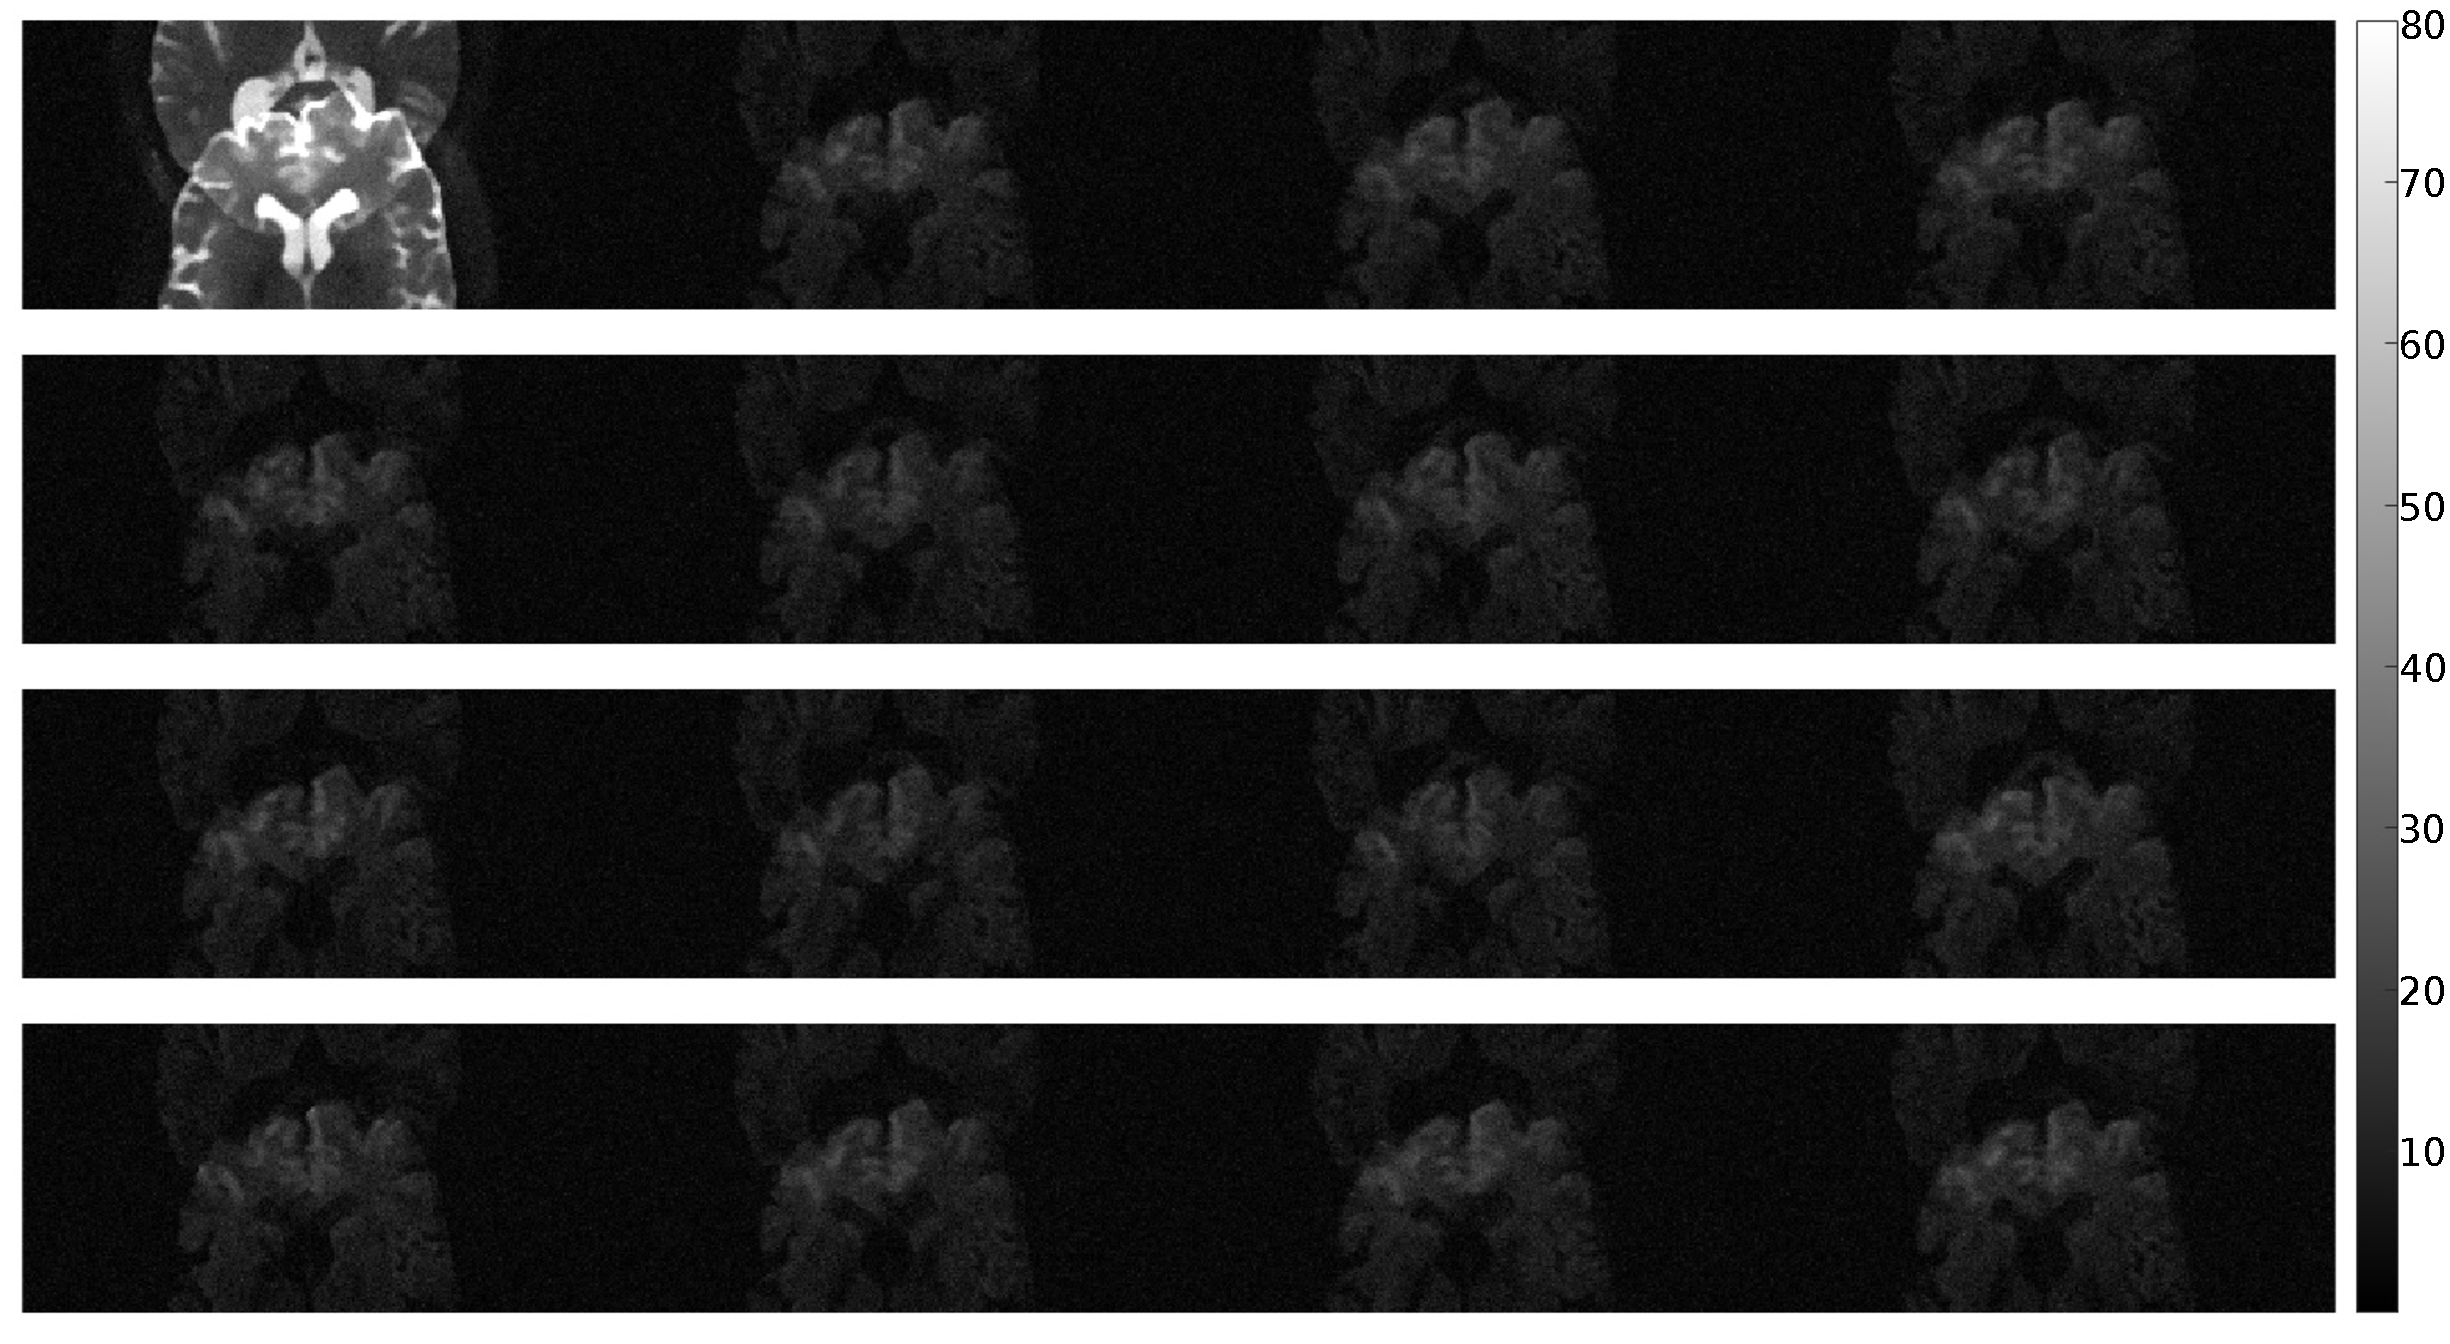
\includegraphics[scale=0.36]{figures/Module_01/NON_RECON.pdf}
  \caption{Subsampled diffusion dataset in \textbf{x}-space domain (data for one particular slice, acquired for 15 diffusion weightening gradients).}
  \label{rys:subsampled}
\end{figure}

\begin{figure}[h!]
\centering
  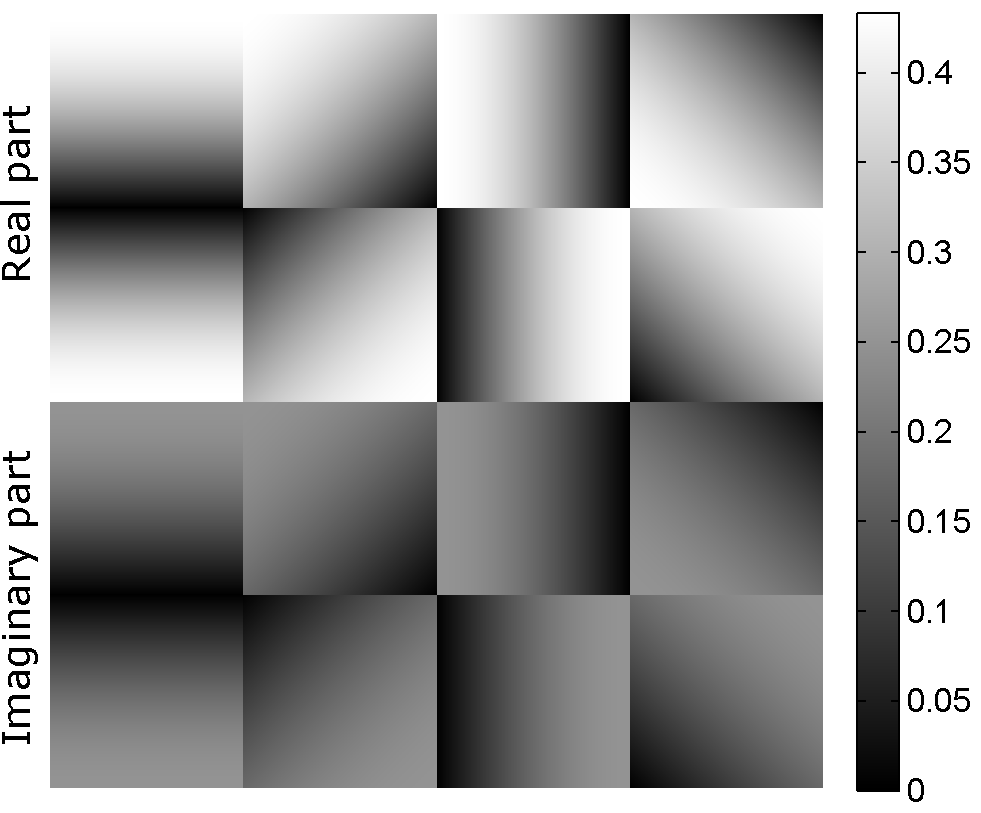
\includegraphics[scale=0.46]{figures/Module_01/MAPS.pdf}
  \caption{The real and imaginary parts of sensitivity maps used to reconstruct data ($L = 8$).}
  \label{rys:maps}
\end{figure}

\begin{figure}[h!]
\centering
  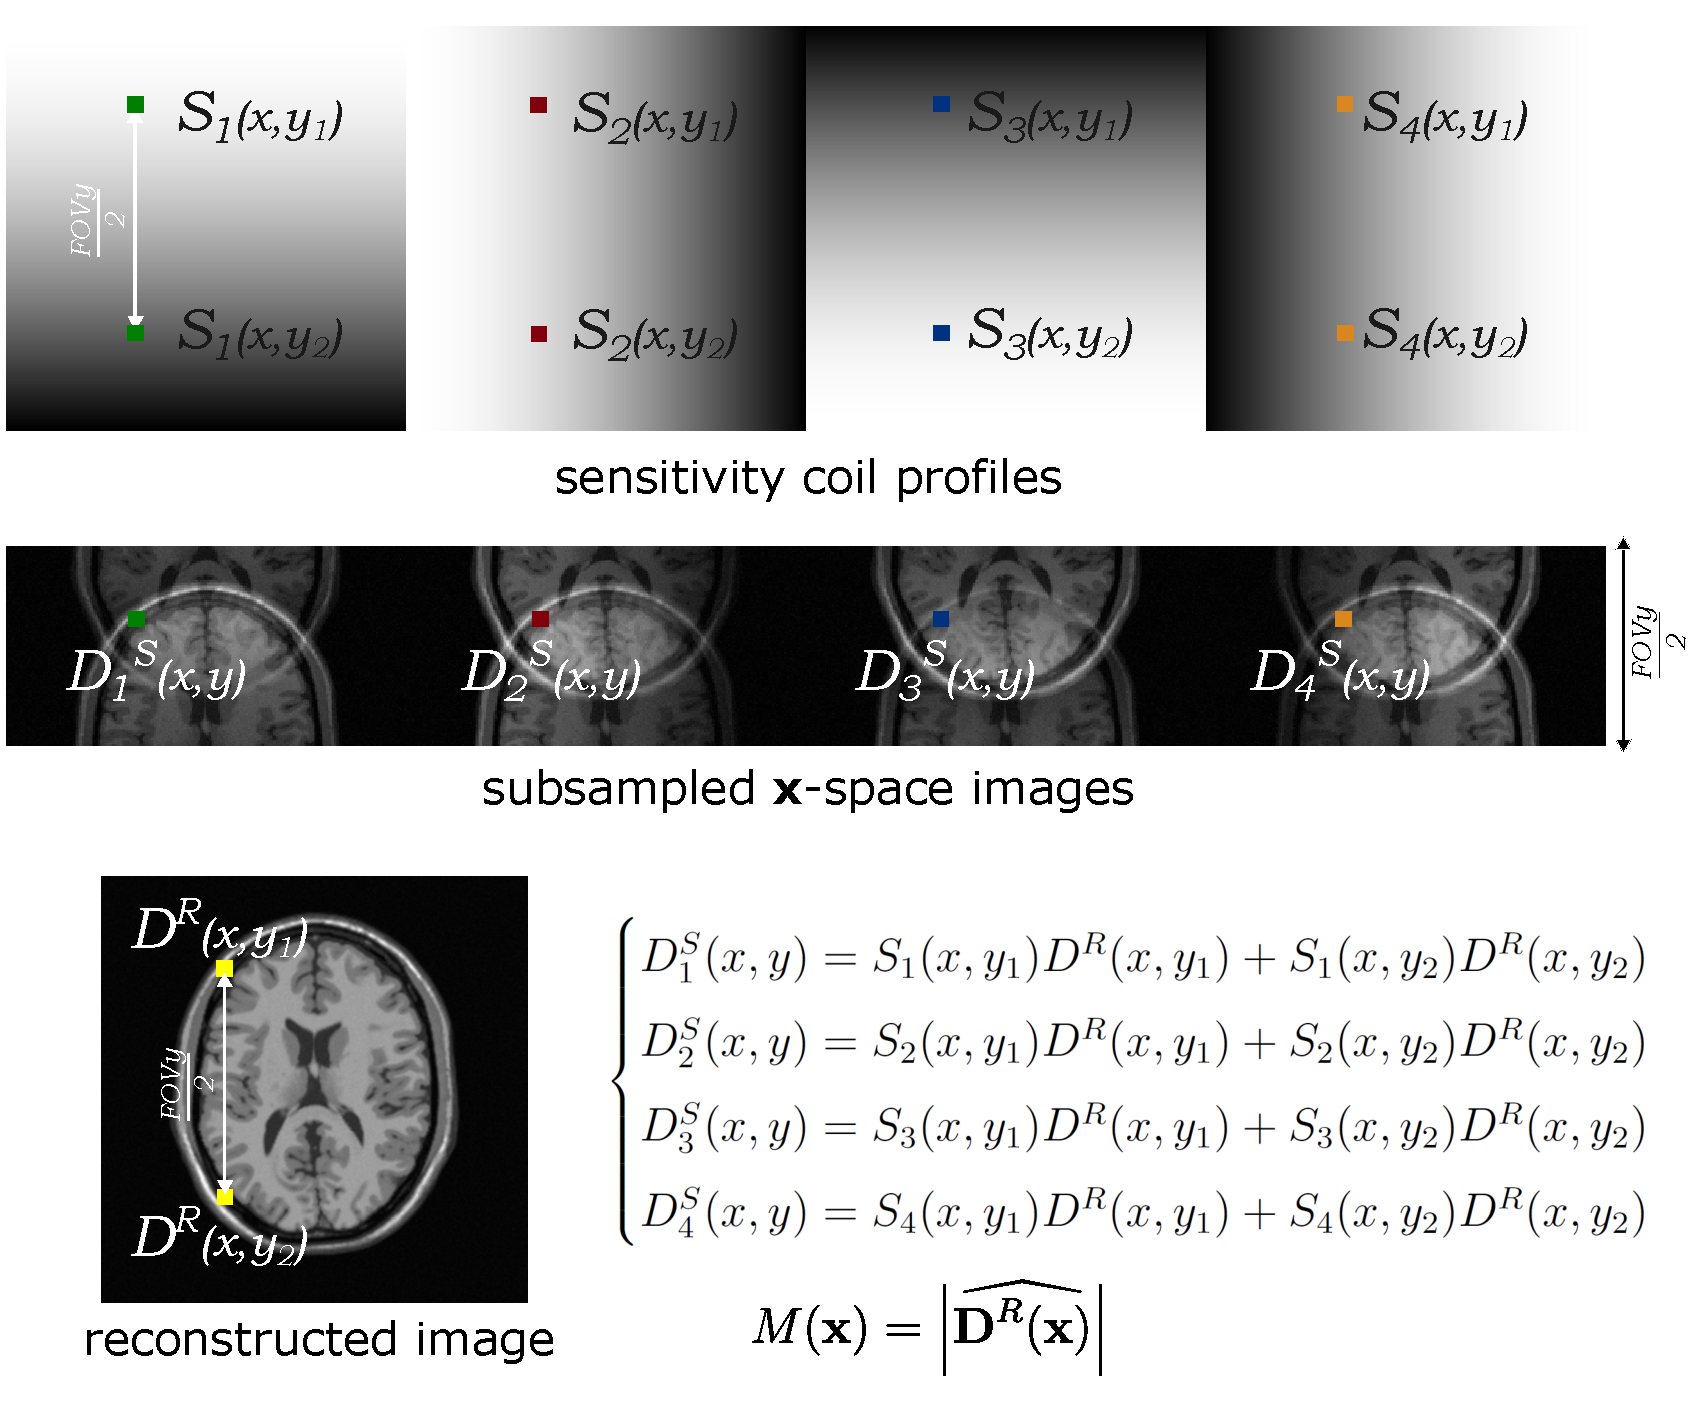
\includegraphics[scale=0.36]{figures/Module_01/SENSE.pdf}
  \caption{SENSE algorithm graphical explanation of Cartesian sampling using four receiver
coils ($L = 4$) and the subsampling rate $r = 2$. Two yellow pixels of the reconstructed image are
unfolded using coil sensitivity profiles and the corresponding folded pixels (points marked with
green, red, blue and orange).}
  \label{rys:sense}
\end{figure}

Thirdly, we used absolute value operator right before performing the SENSE reconstruction main step. As we are provided with sensitivity maps profiles (Fig. \ref{rys:maps}), we can easily reconstruct the subsampled data as it is shown in Fig. \ref{rys:sense}.
The key idea is to evaluate the algorithm pixel by pixel. According to equation \ref{Eq:wzor4}, the construction of defined $\textbf{D}^{S}$ vector is simple. Basically, the $\textbf{D}^{S}$ is a column vector of $L\times1$ size, containing pixels withdrawn from each $L$ coil image at specified spatial location. The matrix $\textbf{S}$ we construct in a~subsequent way: the $l-th$ row of $\textbf{D}^{S}$ contains values of the sensitivity maps profiles, corresponding to data position in a subsampled image and moved by a subsampled FOV value (i.e. for $r=4$, $FOV_{y} = 256/4 = 64$) $r-1$ times. As a result, depending on the number of coils and subsampling rate value, we obtained a matrix of $L\times r$ size. In LSE sense, the result of computation of  for defined $\textbf{D}^{S}$ and~$\textbf{S}$ is column vector $\textbf{D}^{R}$ ($r\times 1$ size). 

However, the LSE approach is not an optimal solution, so we implemented the regularization approach which uses the \textit{a priori} information of searched solution obtained with LSE algorithm. The images obtained after first reconstruction are median filtered with window size$3$x$3$. We introduced this additional information to the solution of derived objective function according to Eq. \ref{Eq:wzor7}. In this case, $\textbf{D}^{S}$ and~$\textbf{S}$ are constructed in the same manner as for LSE case, however we regularized the solution with $\lambda$ parameter. The choice of appropriate value of regularization parameter allows controlling the balance between both components (bias-variance tradeoff). For this scenario, we empirically picked $\lambda$ parameter as a constant value. As the reconstruction is performed pointwisely, we introduced extra information about expected result as a vector $\textbf{D}$ of $r$x$1$ size, containing pixels from reconstructed median filtered LSE images corresponding spatially to those to be reestimated with Tikhonov approach. The result is similar, i.e., we derived values of $r$ reconstructed points, which differ from those obtained with basic LSE approach. Fig. \ref{rys:recon} presents exemplary result of Tikhonov reconstruction algorithm implemented in the software. 

\begin{figure}[h!]
\centering
  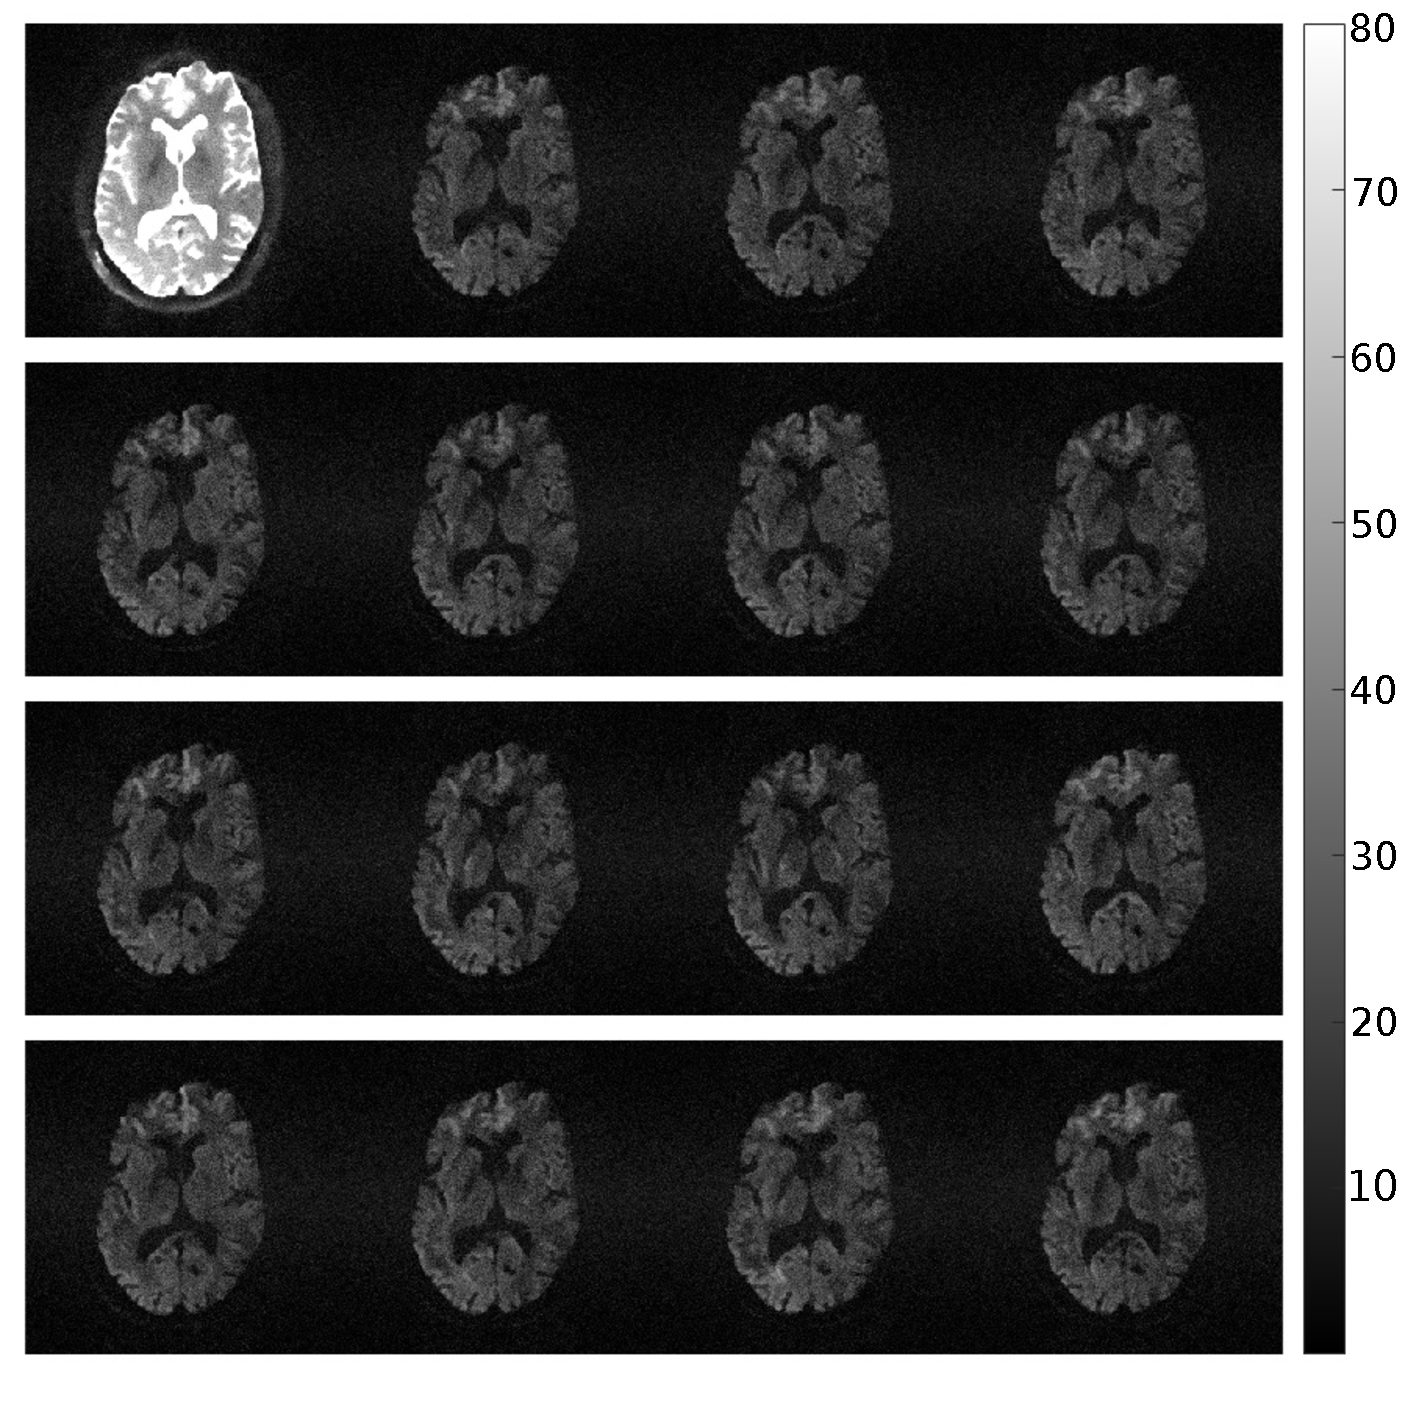
\includegraphics[scale=0.36]{figures/Module_01/RECON.pdf}
  \caption{Reconstructed diffusion dataset in \textbf{x}-space domain (data for one particular slice, acquired for 15 diffusion weightening gradients).}
  \label{rys:recon}
\end{figure}



\section{Module 2. Intensity inhomogeneity correction}

The Intensity inhomogeneity of the same tissue varies with the location
of the tissue within the image. In other words it refers to the slow,
nonanatomic intensity variations of the same tissue over the image
domain. It can be due to imaging instrumentation (such as radio-frequency
nonuniformity, static field inhomogeneity, etc.) or the patient movement.
This artifact is particularly severe in MR images captured by surface
coils. Although intensity inhomogeneity is usually hardly noticeable
to a human observer, many medical image analysis methods, such as
segmentation and registration, are highly sensitive to the spurious
variations of image intensities.

The aim of this module is estimation of intensity inhomogeneity field in MR image using surface fitting method. The method fits a parametric surface to a set of image features that contain information on intensity inhomogeneity. The resulting surface, which is usually polynomial or spline based, represents the multiplicative inhomogeneity field that is used to correct the input image.

The steps of this approach are: 
\begin{enumerate}
\item {Extract a background image from the corrupted MRI image, for example, by smoothing the image with a Gaussian filter of a large bandwidth (about 2/3 the size of the MRI image) to filter out all the image details that correspond to highfrequency components.}
\item {Select few data points from the background image and save their coordinates and graylevel values into a matrix $D = (xi , yi , gi), i = 1, 2, ...n$. It is recommended not to select points from the regions where there is no MRI signal since this regions has no bias field signal.}
\item {Select a parametric equation for the fitted surface . It is better to fit simple surfaces such as low order polynomial surfaces since they are very smooth and their parameters are very easy to estimate.}
\item {Estimate the parameters of the surface that best fits the data in matrix D by the method of nonlinear least-squares.}
\item {Use the fitted equation to generate an image of the bias field signal.}
\item {Divide the corrupted MRI image by the estimated bias field image in step 5.} 
\end{enumerate}
Even though different surfaces can reasonably fit the data very well and it is not possible to tell which surface is most likely represents the actual bias field signal, however, in practice the bias signal estimated by fitting a smooth 2-dimensional polynomial surface to a background image can be used effectively to restore the corrupted MRI image.

Fitting of the surface can be done by means of the Levenberg-Marquardt algorithm for nonlinear least squares fitting of a function $f(x, y; a_{1}, ..., a_{m})$ of known form to $n$ data points ${(x_{1}, y_{1}, g_{1}), ...,(xn, yn, gn)}$. For example, a polynomial surface of degree three can be fitted which has the following equation: $f(x, y; a) = a_{1}x^{3} + a_{2}y^{3} + a_{3}$, where $a = {a_{1}, a_{2}, a_{3}}$ is the parameter vector that define the surface. If we substitute the data points in the nonlinear function we get an overdetermined set of equations, i.e.,
\begin{equation}
\begin{Bmatrix}
g_{1} = f(x_{1}, y_{1}; a_{1}, a_{2}, ..., a_{m})\\ 
\cdot                                            \\
\cdot                                            \\ 
g_{n} = f(x_{n}, y_{n}; a_{1}, a_{2}, ..., a_{m})\\ 
\end{Bmatrix}
\end{equation}
These equations can be solved to obtain the unknown parameter vector $(a_{1}, a_{2}, ..., a_{m})$ by minimizing the sum of the squares of the differences between the data and the fitted function
\begin{equation}
\begin{aligned}
Q(\textbf{a})=\dfrac{1}{2} \sum_{i=1}^{n}(g_{i} - f(x_{i},y_{i}; a_{1},a_{2}, ...,a_{m}))^{2}
\label{fig: eq2_1}
\end{aligned}
\end{equation}
Let $r_{i}(\textbf{a}) = (g_{i} - f( x_{i}, y_{i}; a_{1}, a_{2}, ..., a_{m})$, which is the residual vector of point $i$, then equation \ref{fig: eq2_1} can be written as:
\begin{equation}
\begin{aligned}
Q(\textbf{a})=\dfrac{1}{2} \sum_{i=1}^{n}(r_{1}(\textbf{a}))^{2}
\label{fig: eq2_2}
\end{aligned}
\end{equation}
According to the Levenberg-Marquardt algorithm, eq.\ref{fig: eq2_2} can be solved iteratively to find the values of the parameters vector ($\textbf{a}$) starting from an initial estimate of the parameter vector $(\textbf{a}_{0})$ using:
\begin{equation}
\begin{aligned}
\textbf{a}_{i+1} = \textbf{a}_{i} - (H + \lambda diag[H])^{-1} \bigtriangledown Q(\textbf{a}_{i})
\label{fig: eq2_3}
\end{aligned}
\end{equation}
where $H$ and $\bigtriangledown$Q($\textbf{a}_{1}$) are Hessian matrix and the gradient of Eq. \ref{fig: eq2_2} both evaluated at $a_{i}$, $diag[H]$ is the diagonal elements of the Hessian matrix. At each iteration, the algorithm tests the value of the residual error  and adjusts $\lambda$ accordingly. \cite{2a1}

\section{Module 3. Non-stationary noise estimation}
In order to test effectiveness of implemented algorithm the results of it were compared to results of algorithm prepared to perforem calculatioans contained in \cite{aja2015spatially}. The algorithm for the article was implemented in Matlab.
\begin{figure}[H]
	\centering{}
		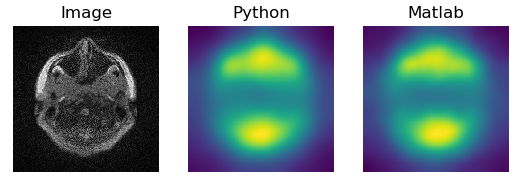
\includegraphics[scale=0.7]{figures/module03/10_comp}
	\caption{Image (left), noise map form Python algorithm(middle), noise map form Matlab algorithm(right).} 
\end{figure}
\begin{figure}[H]
	\centering{}
		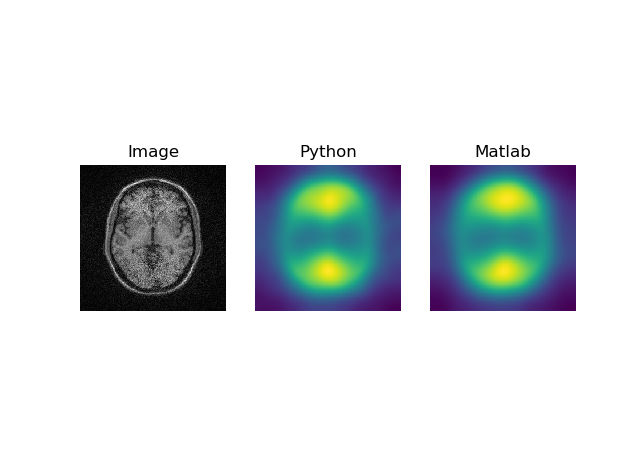
\includegraphics[scale=0.7]{figures/module03/70_comp}
	\caption{Image (left), noise map form Python algorithm(middle), noise map form Matlab algorithm(right).} 
\end{figure}
\begin{figure}[H]
	\centering{}
		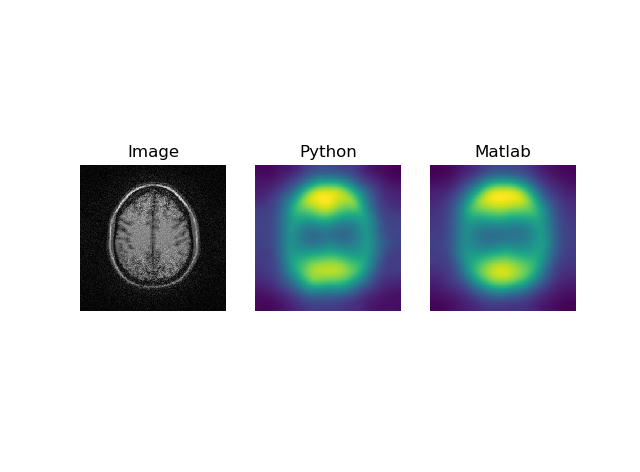
\includegraphics[scale=0.7]{figures/module03/110_comp}
	\caption{Image (left), noise map form Python algorithm(middle), noise map form Matlab algorithm(right).} 
\end{figure}
\begin{figure}[H]
	\centering{}
		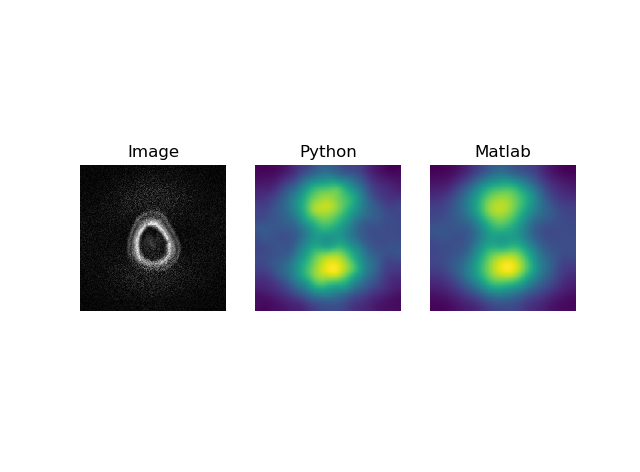
\includegraphics[scale=0.7]{figures/module03/160_comp}
	\caption{Image (left), noise map form Python algorithm(middle), noise map form Matlab algorithm(right).} 
\end{figure}
Results from Python algorithm are not perfect equivalent of the results from Matlab algorithm however ther are very similar and seem to be suitable for 
further processing of the image.

\section{Module 4. Non-stationary noise filtering 1}

The aim of this module is to remove Rician noise from MR images. If
both real and imaginary parts of signal are corrupted with zero-mean
uncorrelated Gaussian noise with equal variance, the envelope of magnitude
signal will follow a Rician distribution. Many processes allow to
remove noise, here the method is used to denoise MR images is the
linear minimum square error estimator (LMMSE). The main purpose of
LMMSE is to find a closed-form estimator for a signal that follows
a Rician distributions. It is more efficient than optimization-based
solutions. The estimator uses information of the sample distribution
of local statistics of the image such as the local mean, the local
variance and the local mean square value. In this method, the true
value for each noisy pixel is estimated by a set of pixels selected
from a local neighborhood.

The LMMSE estimator for a 2-D signal with Rician distribution is defined:

\begin{equation}
\begin{aligned}\widehat{A_{ij}^{2}}=E\{A_{ij}^{2}\}+C_{A_{ij}^{2}M_{ij}^{2}}C_{M_{ij}^{2}M_{ij}^{2}}^{-1}(M_{ij}^{2}-E\{M_{ij}^{2}\})\end{aligned}
\label{m4eq1}
\end{equation}
where $A_{ij}$ is the unknown intensity value in pixel $ij$, $M_{i}j$
the observation vector, $C_{A_{ij}^{2}M_{ij}^{2}}$ the cross-covarience
vector and $C_{M_{ij}^{2}M_{ij}^{2}}$ the covarience matrix. If the
estimator is simplified to be pointwise, vectors and matrics become
scalar values. Then the assuming local ergodicity with a square nighbourhood
around the pixel $ij$, the finally equation for LMMSE is defined:
\begin{equation}
\begin{aligned}\widehat{A_{ij}^{2}}=\langle M_{i}j^{2}\rangle-2\sigma_{n}^{2}+K_{ij}(M_{ij}^{2}-\langle M_{ij}^{2}\rangle)\end{aligned}
\label{m4eq2}
\end{equation}
with $K_{ij}$ 
\begin{equation}
\begin{aligned}K_{ij}^{2}=1-\frac{4\sigma_{n}^{2}(\langle M_{i}j^{2}\rangle-2\sigma_{n}^{2})}{\langle M_{i}j^{4}\rangle-{\langle M_{i}j^{2}\rangle}^{2}}\end{aligned}
\label{m4eq3}
\end{equation}

The LMMSE estimator is related to the quality of the estimate of the
noise variance $\sigma_{n}^{2}$. For the noise estimation the mode
of the sample mean is used:

\begin{equation}
\begin{aligned}\widehat{\sigma_{n}}=\sqrt{\frac{2}{\pi}}mode(\widehat{\mu_{1}}_{ij})\end{aligned}
\label{m4eq4}
\end{equation}
where $\widehat{\mu_{1}}_{ij}$ 
\begin{equation}
\begin{aligned}\widehat{\mu_{1}}_{ij}=\frac{1}{|\eta_{ij}}\sum_{p\colon\eta_{ij}}I_{p}\end{aligned}
\label{m4eq5}
\end{equation}

The use of the LMMSE method should makes the filtering process computationally
far more efficient and easier to implement. Also the use of local
statistics should decrease estimator dependent of parameters such
as the size of window.

\textbf{\emph{Module input}}: Reconstructed, normalized and corrected
data.

\textbf{\emph{Module output}}: Image without Rician noise.

\section{Module 5. Non-stationary noise filtering 2}

Magnetic Resonance images are endangered of being corrupted by noise
and artifacts. Since they are used as a basis for medical diagnosis
their quality has to be at highest possible level. Noise can be dealt
with by changing the parameters of images acquisition, however it
increases the scanning time, which is undesirable in medical imaging.
To overcome this obstacle, post-processing methods like filtering
are employed for denoising. In domain of MRI denoising many filters
may be used, though here emphasis is put on Unbiased Non-Local Means
(UNLM) filter, which is an extension of NLM filter. In order to understand
Unbiased version of this algorithm, the basic one has to be presented.

Having image \textit{Y}, the NLM algorithm calculates the new value
of point \textit{p} accordingly to the equation:

\begin{equation}
\begin{aligned}NLM(Y(p))=\sum_{\forall q\in Y}^ {}w(p,q)Y(q)\\
0\le w(p,q)\le1,\sum_{\forall q\in Y}^ {}w(p,q)=1
\end{aligned}
\label{m5e1}
\end{equation}

It can be seen that value of \textit{p} is calculated as weighted
average of pixels in the image (\textit{q}), having fulfilled restrictions
from \ref{m5e1}. To determine before mentioned average the similarity
between square neighbourhoods widows centered around pixels \textit{p}
and \textit{q} are calculated. The size of the window can determined
by the user, defined by parameter $R_{sim}$. Equation \ref{m5e2}
shows how to determine this similarity.

\begin{equation}
w(p,q)=\frac{1}{Z(p)}e^{\dfrac{d(p,q)}{h^{2}}}\label{m5e2}
\end{equation}

\textit{Z(p)} is the normalizing constant which also uses exponential
decay parameter \textit{h} and the weighted Euclidean distance measure
for pixels in each neighbourhood, called \textit{d}.

\begin{equation}
Z(p)=\sum_{\forall q}^ {}e^{\dfrac{d(p,q)}{h^{2}}}\label{m5e5}
\end{equation}

\begin{equation}
d(p,q)=G_{p}||Y(N_{p})-Y(N_{q})||_{R_{sim}}^{2}\label{m5e6}
\end{equation}

In above equation $G_{p}$ stands for a Gaussian weighting function
that has a 0 mean and standard deviation usually equal to 1.


Once NLM filter is fully explained, unbiased extension of it can be
examined. It builds on the properties of MRI signal. According to
\cite{5a1} the magnitude signal of MRI follows a Rician distribution.
Furthermore, for low intensity regions the Rician distribution approaches
to a Rayleigh one, whilst for high intensity it shifts towards Gaussian.
It was investigated that this bias can be handled by filtering the
squared MRI image, since it is not longer signal-dependent \cite{5a1}.
As a consequence the bias, which equals 2$\sigma^{2}$ \cite{5a3}
can be deleted with ease. The blueprint for UNLM can be summarized
in:
\begin{itemize}
\item noise estimation - which can be done by calculating standard deviation
of background in the image. To distinguish
background and the body on the MRI scan the Otsu thresholding method
\cite{5a4} can be successfully used. In this version noise maps are used, to achieve
non-stationary noise filtration, 
\item calculating NLM values for each point of image as in \ref{m5e1}, 
\item assessing the unbiased value of each point accordingly to the equation
\ref{m5e3}.
\end{itemize}
\begin{equation}
UNLM(Y)=\sqrt{NLM(Y)^{2}-2\sigma^{2}}\label{m5e3}
\end{equation}

In above equation $\sigma$ refers to value of non-stationary noise in the signal, more precisely
it is a value for each pixel from the original image, stored in a form of noise map.

% dwi, if it has to be joint implementation 
UNML implementation for diffusion weighted data becomes a bit less
trivial task, due to the new dimension of data associated with different gradients for each slice.
Based on assumption that gradients in similar directions
present related behaviours, UNLM for DWI can be formulated as:

\begin{equation}
Y_{i}(p)=\sqrt{\sum_{j\in\Theta_{i}^{N}}^ {}\sum_{q\in N_{p}}^ {}w_{i}^{j}(p,q)M_{j}^{2}(q)-2\sigma^{2}}
\end{equation}

Where weights are calculated as for structural data and \textit{M}
is a vector containing gray values.

\begin{equation}
d_{i}^{j}(p,q)=(M_{i}(N_{p})-M_{j}(N_{q}))^{T}G_{p}(M_{i}(N_{p})-M_{j}(N_{q}))\label{m5e7}
\end{equation}

However it was reported in \cite{5a2} that denoising diffusion weighted data using
UNLM method gives no significant results, so gradients related data can be ignored, or 
filtered as structural data.

It is worth mentioning that UNLM filter's performance is highly dependent
on parameter values. The optimal values of them were examined in \cite{5a1}
and same values are adapted in presented implementation. Properly-tuned
filter can significantly increase SNR of the scans while preserving
body structures.

\textbf{\emph{Module input}}: Previously reconstructed, normalized
and corrected data, noise maps.

\textbf{\emph{Module output}}: Image with deleted Rician noise by
unbiased non-local means filter. \\

\section{Module 6. Diffusion tensor imaging}

\textbf{Preprocessing and Module I/O}

In order to improve diffusion tensor estimation it is imperative to
remove artifacts. In addition to standard MRI pre-processing, one
needs to correct for artifacts arising the use of diffusion-gradient
pulse sequences and longer acquisition time. While hardware manufacturers
try to proactively diminish some of these effects, software processing
is still mandatory. 
\hfill\\

\textbf{Module Input}:
\begin{itemize}
	\item 
	3D structural data array of shape X x Y x Z, where XY - pixel image intensities, Z - chosen slice, which is the T1- or T2-weighted image corresponding the the given DWI acquisition
	
	\item 
	4D diffusion data array of shape X x Y x Z x M, where XY - pixel image intensities, Z - chosen slice, M - applied diffusion gradient direction
	
	\item 
	b\_value, a scalar value corresponding to applied diffusion gradient sequence magnitude
	
	\item 
	2D gradients matrix of shape M x 3, where each row corresponds to a normalized $(x,y,z)$ components of diffusion gradient sequence vectors
		
	\item 
	optionally - 3D binary mask of shape X x Y x Z, corresponding to the brain area detected by Module 8 (Skull Stripping); if not supplied, DTI is computed on each input data voxel

\end{itemize}
\hfill

\textbf{Module Output}:
\begin{itemize}
	\item
	list of size Z, corresponding to each slice; every list element is a dictionary of biomarker images: MD, RA, FA, VR of shape X x Y, and biomarker FA\_rgb of shape X x Y x 3
\end{itemize}

\subsection{Initialization}

In order to abstract DTI implementation from end-user, all classes and methods other than the main function \texttt{run\_module} are private to module source code script. It is important to note that prior to running the module one has to provide the module with input data object, as well as SOLVER and FIX\_METHOD parameters. SOLVER passed as an argument decides whether to use WLS or NLS estimation, whole FIX\_METHOD decides how to "fix" negative eigenvalues. 

As mentioned in the detailed description chapter, 'ABS' takes absolute value of each eigenvalue, while 'CHOLESKY' ensures that the estimated tensor is positive definite. Eigenvalues of positive definite matrices are always non-negative. 'ABS' is a post-estimation fix, meaning that it does not modify the default estimation algorithm (i.e. it is applied after WLS or NLS computation), while 'CHOLESKY' directly modifies the expressions for WLS and NLS cost function gradients and Hessian matrices.

After passing all required arguments to the \texttt{run\_module} function, they are reshaped internally in order to be compatible with module. Concretely, \texttt{DTISolver} class instance, computing the DTI proper, assumes that input data argument is a concatenated 3D array of both structural and diffusion images, which are stored separately in the original data structure. Moreover, b\_value and gradient fields are reshaped to be lists correpsonding to each slice of the new data array (that is: b\_value is repeated in length while both have zeros appended that correspond to structural images). Finally, all of the above is done separately for each slice and DTI module performs it's computation slice-by-slice due to memory constraints.

\subsection{WLS estimation}

WLS with the ABS fix method is a fast yet simple method of module pipeline computation based on diffusion tensor estimation. As such these parameters were set as default for DTI.

Diffusion tensor estimate was computed by implementing the equation:
\begin{equation}
\begin{aligned}
\boldsymbol{\gamma}=\left(\boldsymbol{W}^T\boldsymbol{\omega}^T\boldsymbol{\omega}\boldsymbol{W}\right)^{-1}\boldsymbol{W}^T\boldsymbol{\omega}^T\boldsymbol{\omega y}
\end{aligned}
\label{Eq:m6_impl_eq_1}
\end{equation}

using NumPy matrix broadcasting operations, effectively abstracting away array reshaping. Weights vector $\boldsymbol{\omega}$ is calculated using a separate function in order to avoid changing every piece of code refering to WLS weights in case they change. The following implementation assumes the simplest of models presented in the Detail Description chapter, that is weights being equal to the measured signal.

\subsection{NLS estimation}

In case of NLS estimation, in addition to implementing gradient and Hessian matrix computation methods:

\begin{equation}
\begin{aligned}
\nabla{f_{NLS}}&=-\boldsymbol{W}^T\boldsymbol{\hat{S}}\boldsymbol{r} \\
\nabla^2{f_{NLS}}&=\boldsymbol{W}^T\left(\boldsymbol{\hat{S}^T\hat{S}-\boldsymbol{R\hat{S}}}\right)\boldsymbol{W}
\end{aligned}
\label{Eq:m6_impl_2}
\end{equation}

It is important to devise an iterative scheme because gradient result depends on NLS diffusion tensor estimate. For that reason an algorithm based on \cite{m6_koay2006a} has been implemented. The method itself is called a Modified Newton's Algorithm and can be summarised as in Fig.\ref{fig:m6_pic_1}.

\begin{figure}[H]
	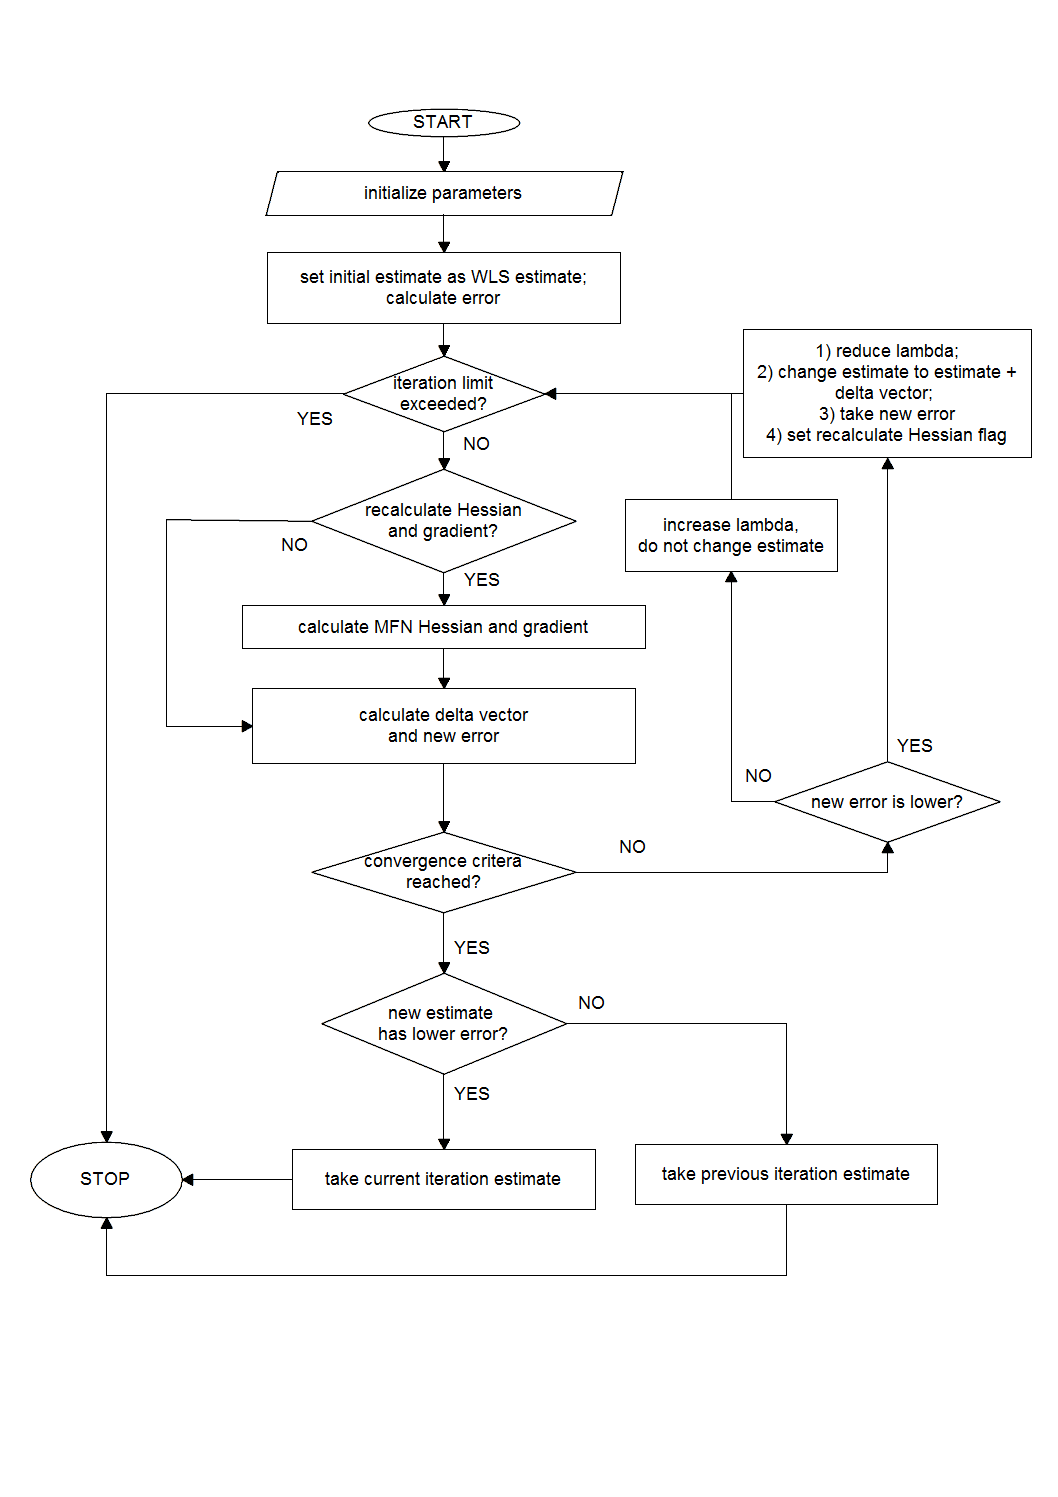
\includegraphics[width=8cm]{figures/Module_06/mfn_simple}
	\centering
	\caption{Modified Newton's method for iterative computation of NLS estimate \vbox{(based on \cite{m6_koay2006a})}}.
	\label{fig:m6_pic_1}
\end{figure}

The following parameters (collectively known in code as MFN parameters) were set:
\begin{itemize}
	\item 
	MFN\_MAX\_ITER = 3 - iteration limit
	
	\item
	MFN\_ERROR\_EPSILON = 1e-5 - first convergence criterion (error change is small)
	
	\item
	MFN\_GRADIENT\_EPSILON = 1e-5 - second convergence criterion (vanishing gradient)
	
	\item
	MFN\_LAMBDA\_MATRIX\_FUN = 'identity'- regularization matrix added to Hessian matrix
	
	\item 
	MFN\_LAMBDA\_PARAM\_INIT = 1e-4 - initial regularization matrix multiplier
\end{itemize}

Delta estimate is calculated using the following formula:
\begin{equation}
\boldsymbol{\delta}=-\left(\nabla^2{f_{NLS}+\lambda I}\right)^{-1}\nabla{f_{NLS}}
\label{Eq:m6_impl_3}
\end{equation}

with $\lambda$ parameter increasing and decreasing by a factor of 10, depending on whether newly calculated estimate yields lower error (decreasing for lower error, increasing otherwise).

Convergence is established using the following formulas:
\begin{equation}
\begin{aligned}
\left|f_{NLS_{new}} - f_{NLS_{new}}\right| &< \texttt{MFN\_ERROR\_EPSILON} \\
\delta^T\nabla{f_{NLS}} &< \texttt{MFN\_GRADIENT\_EPSILON}
\end{aligned}
\end{equation}

\subsection{Biomarkers computation}

As mentioned previously, the estimate obtained from NLS or WLS methods can be reshaped to a 3x3 matrix:
\begin{equation}
\boldsymbol{D}=
\begin{bmatrix}
D_{xx} & D_{xy} & D_{xz} \\
D_{yx} & D_{yy} & D_{yz} \\
D_{zx} & D_{zy} & D_{zz} 
\end{bmatrix}
\label{Eq:m6_impl_4}
\end{equation}
assuming our estimate is equivalent to:
\begin{equation}
\boldsymbol{\gamma}={\lbrack ln{S_0}, D_{xx}, D_{yy}, D_{zz}, D_{xy}, D_{yx}, D_{xz}\rbrack}^T
\label{Eq:m6_impl_5}
\end{equation}

Tensor estimation results for a sample 126x126x55 slice are presented on Fig.\ref{fig:m6_pic_2}.

\begin{figure}[H]
	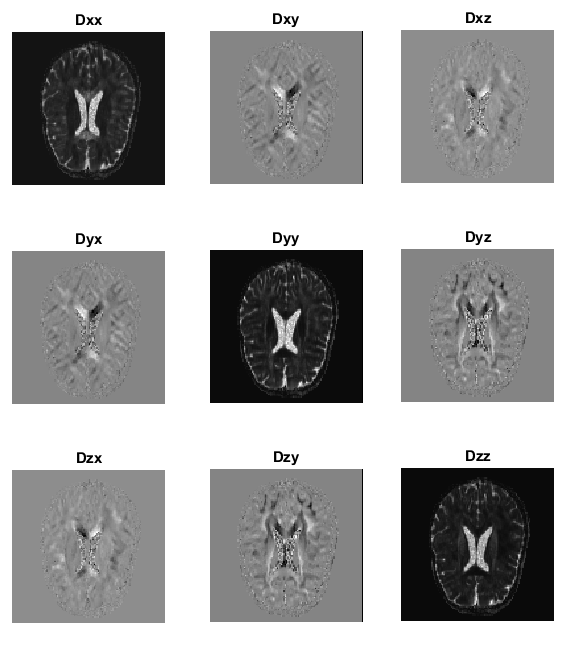
\includegraphics[width=16cm]{figures/Module_06/tensor_image}
	\centering
	\caption{Diffusion tensor estimate using the WLS-ABS method for a 126x126x55 test image.}
	\label{fig:m6_pic_2}
\end{figure}

We can then compute the eigenvalue decomposition of $\boldsymbol{D}$ and obtain eigenvalues and eigenvectors for each pixel of input image. Eigenvalues are sorted in descending order and saved for later computation (Fig.\ref{fig:m6_pic_3}). Moreover, eigenvectors corresponding to the highest eigenvalue are saved to separate variable, since they represent the direction of principal diffusion.

\begin{figure}[H]
	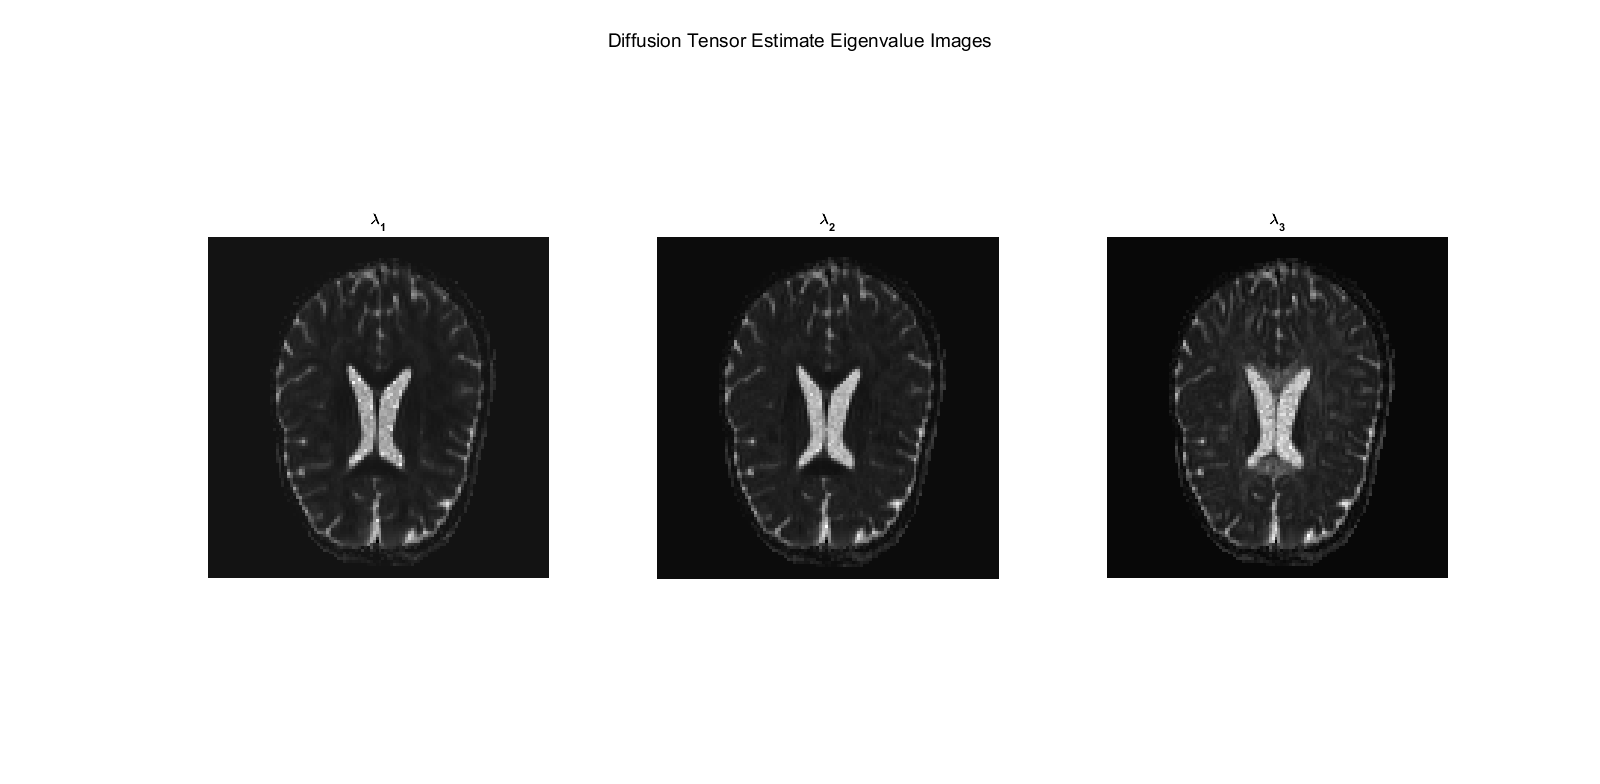
\includegraphics[width=16cm]{figures/Module_06/eig_image}
	\centering
	\caption{Diffusion tensor estimate eigenvalues of sample imgae; eigenvalues sorted in descending order from left to right.}
	\label{fig:m6_pic_3}
\end{figure}

Biomarkers are then computed using the following formulas:
\begin{equation}
MD = \dfrac{\lambda_{1}+\lambda_{2}+\lambda_{3}}{3}
\end{equation}
\begin{equation}
RA = \sqrt{\dfrac{\left(\lambda_{1}-MD\right)^2+\left(\lambda_{2}-MD\right)^2+\left(\lambda_{3}-MD\right)^2}{3\,MD}}
\end{equation}
\begin{equation}
FA = \sqrt{\dfrac{3}{2}}\sqrt{\dfrac{\left(\lambda_{1}-MD\right)^2+\left(\lambda_{2}-MD\right)^2+\left(\lambda_{3}-MD\right)^2}{\lambda_{1}^2+\lambda_{2}^2+\lambda_{3}^2}}
\end{equation}
\begin{equation}
VR = \frac{\lambda_{1}\lambda_{2}\lambda_{3}}{MD\,^3}
\end{equation}

Computed biomarkers of the sample image are presented on Fig.\ref{fig:m6_pic_4}. It is important to note that skull is visible because the brain area was selected by hand instead of relying on Module 08 output.

\begin{figure}[H]
	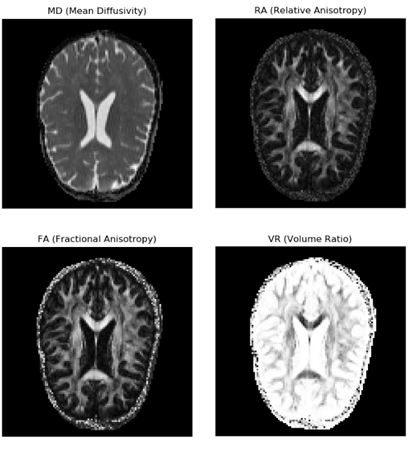
\includegraphics[width=12cm]{figures/Module_06/biomarkers_wls}
	\centering
	\caption{Diffusion biomarkers of sample image. Top left: MD, top right: RA, bottom left: FA, bottom right: VR.}
	\label{fig:m6_pic_4}
\end{figure}

Figure \ref{fig:m6_pic_5} presents the fifth biomarker image present in output dictionary - FA-weighted principal direction of diffusion color map. Color-encoded direction for this slice is presented as follows:
\begin{itemize}
	\item 
	red - transversal (left-right)
	
	\item 
	green - anterior-posterior (front-back)
	
	\item
	blue - cranio-caudal (head-feet)
\end{itemize}

\begin{figure}[H]
	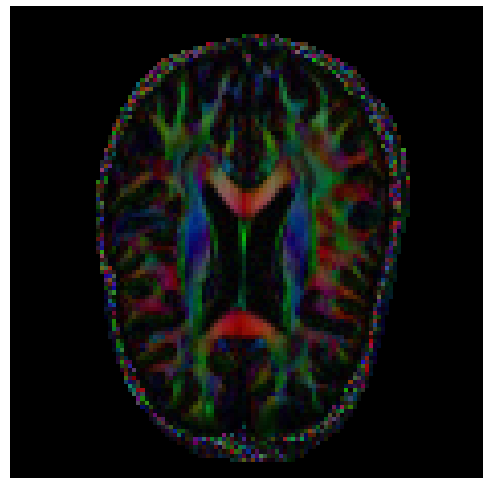
\includegraphics[width=10cm]{figures/Module_06/fa_rgb}
	\centering
	\caption{FA-weighted principal direction of diffusion of sample image.}
	\label{fig:m6_pic_5}
\end{figure}

\subsection{Implementation caveats}

Module source code was implemented and tested on a single sample image outlined above. It constituted a perfect basis for algorithm evaluation because it was already preprocessed, without the need to wait for other modules implementation. Even though it lacked a skull stripping mask, hand-drawn shape was good enough for testing, even though skull outline is visibly present, particularily on Fig.\ref{fig:m6_pic_5}. 

It was difficult to determine which estimation method - WLS or NLS - is objectively better. WLS was significantly faster and it was not much different from NLS results. This might have been due to the fact, that the diffusion-encoding gradient matrix was unusually large (7 structural images and 48 DWIs). Testing on preprocessed raw data, supplied for application evaluation has shown differences between methods, although both estimates are valid (to the Author's best knowledge) as it is difficult to compare any estimation methods without reference.

Initially developed using nested for-loops, DTI module has been vectorized to speed up computations. For a supplied 256x256x16 DWI stack a single slice is being processed in less than 3 seconds for WLS-ABS, while other methods scale linearily with chosen number of iterations (starting at 6 seconds, then 3 seconds per MFN iteration). It must be noted that the module was not tested with skull stripping mask, which could have drastically reduced computation time. Moreover computation time heavily depends on hardware constraints.

\section{Module 8. Skull stripping}

Preliminary processing to isolate the brain form extra-cranial or non-brain tissues such as e.g. the eye sockets, skin from MRI head scans is commonly referred as skull stripping. Skull stripping methods which are available in the literature are broadly classified into five categories: mathematical morphology-based metods, intensity-based methods, deformable surface-based methods, atlas-based methods, and hybrid methods. Each skull stripping method has their own merits and limitations.
The aim of this module is to remove pieces of skull from MRI Image using at pleasure chosen algorithm from the literature. Skull stripping is performed with use of two methods:
\begin{itemize}
    \item {Brain Surface Extractor BSE proposed by Stattuck et al. [1]}
    \item {Marker-controlled watershed algorithm by Abdallah and Hassan and by Segonne et al. [2], [3]}
\end{itemize}
Before this methods, there is applying preprocessing function to estimate global parameters: CSF - an upper bound for the intensity of the cerebrospinal fluid, COG - the coordinates of the centroid of the brain, BR - the average brain radius and ratio to brain diameter in axis x to brain radius in axis y. These estimated parameters are useful in this to methods to optimization and working.
BSE procedure consist of three steps:
\begin{enumerate}
\item {The MRI is processed with anisotropic diffusion filter to smooth nonessential gradients.}
\item {The filtered image has applied a Marr-Hildreth edge detector to identify important anatomical boundaries.}
\item {Using a sequence of morphological and connect component operation to define object by previous boundaries.}
\end{enumerate}

Anisotropic Diffusion filtering is applied to smooth noisy regions, which can obscure boundaries or their edges can be indistinguishable from the other in the image. To implement this filter is used an image processing method by Perona and Malik. They demonstrated that using the gradient of image intensity as an estimate of edge strength produces good results. The filtered image is modeled as the solution to the anisotropic diffusion equation
\begin{equation}
    \frac{\partial I}{\partial t} = \nabla \cdot (c(\textbf{p},t)\nabla I) = c(\textbf{p},t)\nabla^{2}I + \nabla c \cdot \nabla I  \label{Eq:wzor_1}
\end{equation}
where \textbf{p} is a point in $R^{2}$, $\nabla$ and $\nabla^{2}$  represent the gradient and Laplacian operators and $\nabla$ $\cdot$ indicates the divergence operator. The function is defined as:
\begin{equation}
    c(\textbf{p},t) = g(\parallel\nabla I(\boldsymbol{p},t)\parallel) = e^{-\parallel\nabla I(\textbf{p},t)\parallel^{2} \kappa^{2}_{d}} \label{Eq:wzor_2}
\end{equation}
where $\kappa_{d}$ is the diffusion constant. \eqref{Eq:wzor_2} gives preferences to high-contrast edges. Number of iteration and the diffusion parameter $\kappa_{d}$ is selected empirically.

To locate the anatomical boundaries in MRI brain volumes, it is used the Marr-Hildreth edge detectors. It is based on a low-pass filtering step with a symetric Gaussian kernel, followed by the localization of zero-crossing in the Laplacian of the filtered image. The Marr-Hildreth operator is defined as:
\begin{equation}
    C(k) = \nabla^{2}(I(k)*g_{\sigma}(\textbf{p})) \label{Eq:wzor_3}
\end{equation}
where C is the output contour image, I is an input image, * is the convolution operator, $g_{\sigma}$ is a Gaussian kernel with variance $\sigma^{2}$
\begin{equation}
    g_{\sigma} = \frac{1}{\sqrt{2\pi}\sigma}e^{- \parallel\textbf{p}\parallel^{2}/2\sigma^{2}} \label{Eq:wzor_4}
\end{equation}
where \textbf{p} is a point in the image, and $\nabla^{2}$ is the Laplacian operator.
To find pixels in the contour image, C where zerocrossing occur, a binary image E is produced that separates the image into edge-differentiated segments. Small values for sigma produce narrow filters, resulting in more edges in the image, on the other hand increasing this value makes the blurring kernel wider and only strong edges remain. This detector output is an image, which edge pixels are black and nonedge ones are white.

Morphological processing’s task is to select the pixels corresponding to the brain tissue from the original image. The output of edge detector often does not distinguish meninges or blood vessels from the brain tissue due to noise, low contrast between brain and meninges or true anatomical continuity. The first step is morphological erosion, which delete narrow connections without globally damaging image. After that the largest connected region centered in the volume consist entirely of brain tissue. Second step is selection of this region. Third step, is binary dilatation to restore the brain due to previous erosion, which decrease brain surface. Because of imperfections in the edge boundaries detection, image after dilatation may consist of pits in its surface or small holes within the surface. The last step of morphological processing is closing, which fill small pits and close of some holes that occur.

Marker-controlled watershed segmentation follows this procedure:
\begin{enumerate}
    \item {Computation a segmentation function.}
    \item {Computation the foreground markers.}
    \item {Computation the background markers.}
    \item {Computation of the watershed transform using of the foreground markers and the background markers.}
\end{enumerate}
First step is applied to find the edges in the image, it is processed with Sobel edge filter. The gradient is high at the borders of the object and low inside. Morphological techniques are used to compute the foreground markers, opening by reconstruction and closing by reconstruction to clean up the image. These operation will create flat regional maxima inside each object that can be used to find regional maxima and next modified them by a closing followed by an erosion to obtain good foreground markers. The background pixels after binarization are black, but their markers should be to close to the edges of the object. this can by done by computing the watershed transform of the distance transform of the binary image and the looking for the watershed ridges lines of the result. With the foreground markers and the background markers there is applied watershed based segmentation.

Brain Surface Extraction and Marker-controlled Watershed Segmentation is working separately. The base method is BSE. Marker-controlled watershed segmentation is compute, when BSE brain mask is larger than a mask based on preprocessing estimated BR.

\hfill{}\\
\textbf{List of References}\\
\cite{8_dti_1}, \cite{8_dti_2}, \cite{8_dti_3}, \cite{8_dti_4},


\section{Module 9. Segmentation}

Brain MRI segmentation is an essential task in many clinical applications
because it influences the entire analysis. This is because different
processing steps rely on accurate segmentation of anatomical regions.
For example, MRI segmentation is commonly used for measuring and visualizing
different brain structures, for delineating lesions, for analysing
brain development, and for image-guided interventions and surgical
planning.

\textit{MRI Processing} To prepare brain MRI for segmentation, it
is necessary to perform several preprocessing steps. (Fig. \ref{fig:Preprocessing}).

\begin{figure}[H]
\centering{}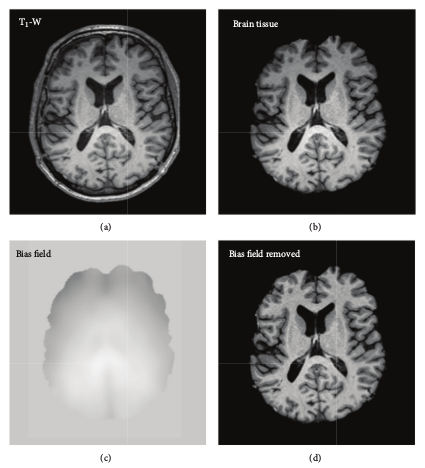
\includegraphics[scale=0.7,bb = 0 0 200 100, draft, type=eps]{9Preprocessing}\caption{Triangulation for the 15 patterns. \label{fig:Preprocessing}}
\end{figure}

The most important steps are: MRI bias field correction, image registration
and brain extraction.

\textit{Basic} An image for segmentation can be defined in 2D space
(pixels) or in 3D space (voxels). Each image element is specified
by its intensity value and coordinates for pixels (i,j) and for voxels
(i,j,k). Intensity values are typically represented by a gray value
{0, …, 255}.

The goal of image segmentation is to divide an image into a set of
semantically meaningful, homogeneous, and nonoverlapping regions of
similar attributes such as intensity, depth, color, or texture. Thesegmentation
result is either an image of labels identifying each homogeneous region
or a set of contours which describe the region boundaries.

Fundamental components of structural brain MRI analysis include the
classification of MRI data into specific tissue types and the identification
and description of specific anatomical structures. The problems of
segmentation and classification are interlinked because segmentation
implies a classification, while a classifier implicitly segments an
image. In the case of brain MRI, image elements are typically classified
into three main tissue types: white matter (WM), gray matter (GM),
and cerebrospinal fluid (CSF) (Fig. \ref{fig:Segment}).

\begin{figure}[H]
\centering{}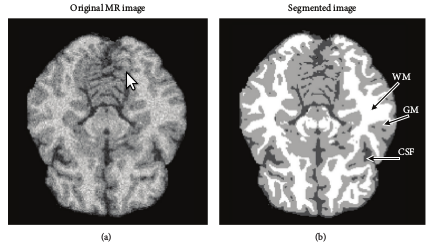
\includegraphics[scale=0.7,bb = 0 0 200 100, draft, type=eps]{9Segmentation}\caption{Triangulation for the 15 patterns. \label{fig:Segment}}
\end{figure}

One of the most important features for brain MRI segmentation is the
intensity of brain tissue. However, intensity-based segmentation algorithms
will lead to wrong results when intensity value are corrupted by MRI
artifacts.

\textit{MRI Segmentation Methods} There is no single method that can
be suitable for all images, nor are all methods equally good for a
particular type of image. For example, some of the methods use only
the gray level histogram, while some integrate spatial image information
to be robust for noisy environments. Some methods use probabilistic
or fuzzy set theoretic approaches, while some additionally integrate
prior knowledge (specific image formation model, e.g., MRI brain atlas)
to further improve segmentation performance. The segmentation methods,
with application to brain MRI, may be grouped as follows: 
\begin{itemize}
\item manual segmentation; 
\item intensity-based methods (including thresholding, region growing, classification,
and clustering); 
\item atlas-based methods; 
\item surface-based methods (including active contours and surfaces, and
multiphase active contours); 
\item hybrid segmentation methods. 
\end{itemize}
\hfill{}\\
\textbf{List of References}\\
\cite{09a1}

\section{Module 10. Upsampling}

The implementation began with making a decision about the input data. The input image has to be 2 dimensional without a noise. The uploaded image will be considered as a 2 dimensional array of double values. Other parameters that will be needed are vertical and horizontal extensions. It has to be a total number. The size of the input array will be multiplied by the number. For example, the image 256x256 pixels with extensions equal to 3 will be 768x768 pixels as an output. The function needs also the window size. In one iteration, the function will take into consideration only pixels witch are inside the window. The loop will stop only when the whole image will be interpolated. To see the results the \textit{plotting} parameter has to be a boolean \textit{True} value. 
\newline The below picture shows the block diagram of the algorithm (Fig. \ref{fig: Module10_4}) with comments added.

\begin{figure}[H]
\centering{}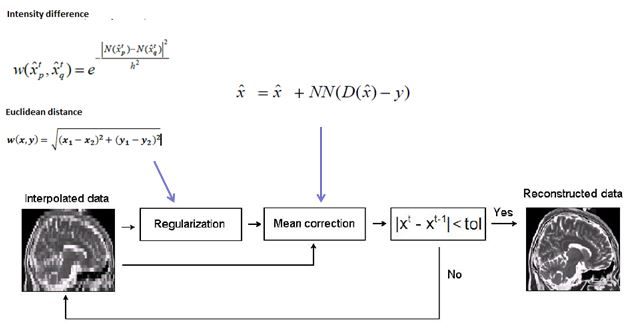
\includegraphics[scale=0.7]{figures/Module_10/Module10_4}\caption{Algorithm block diagram with comments}. 
\label{fig: Module10_4}
\end{figure}

The following steps of the implementation will be discussed:

\begin{enumerate}

\item \textbf{Initial interpolation}
\newline To form the input image into the output with chosen size the initial interpolation is needed. As showed in \cite{9art1} the spline interpolation is used. In short, spline interpolation is an interpolation where interpolant is a special kind of piecewise polynomial called spline. It is recommended, because of the fact that the method makes small error even with low degree polynomials for the spline. Taking into consideration the edges the extrapolation was applied. To be more specific, the last row \textit{n} is equal to the previous one \textit{n-1}. The same with the first row, the first column and the last column of the input. To show the results, the extensions are set as 2. The input data is 256x256 pixels. The undermentioned picture (Fig. \ref{fig: Module10_5}) shows the result of the initial interpolation. The scale is included so it is easy to see that the size is twice as big. Now, the zeros (Fig. \ref{fig: Module9_3}) have  nonzero values, so the next steps can be made.


\begin{figure}[H]
\centering{}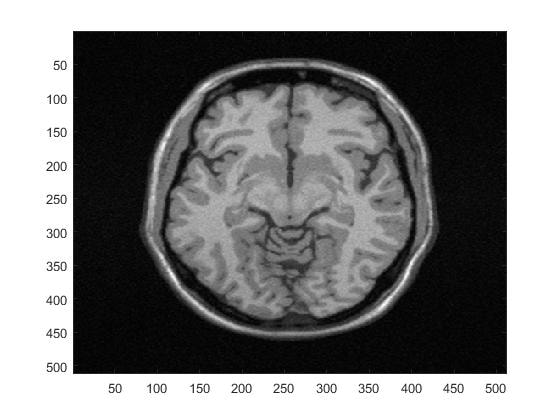
\includegraphics[scale=0.5]{figures/Module_10/Module10_5}\caption{The image after initial interpolation 512x512 pixels}. 
\label{fig: Module10_5}
\end{figure}

\item \textbf{Regularization}
\newline The main functionality is the regularization step. The function makes the square window which contains some pixels. In one iteration of a loop, only the pixels which are inside the window are considered. Next, the window moves and takes another pixels. It is repeated till the end of the image. The main goal is to determine of the weight which will be used at the end.
\newline The first weight is calculated as the difference between the pixels intensities.
\newline 
\centerline {$w_{1}(x, y)= e^{\frac{|N(x)-N(y)|^{2}}{h^{2}}}$, where}
\newline
\newline $N(x)$, $N(y)$ are window and image intensity values,
\newline $h$ is a level, which is equal to the half of the standard deviation of the input image.
\newline The next part of the whole weight is an Euclidean distance weight. It is simply calculated as the Euclidean distance between every pixel in the window and every pixel in the image. It is based on the below equation.
\newline
\centerline{ $w_{2}(x,y)=\frac{\sqrt{(x_{1}-x_{2})^{2}+(y_{1}-y_{2})^{2}}}{h^{2}}$, where }
\newline
\newline $h$ is a level, which is equal to the half of the standard deviation of the input image.
\newline The total weight is calculated as $w_{total}=w_{1}*w_{2}$. The output image is determined as the result of the sum of the multiplication of the weight and the window, divided by the sum of the weight.

\item \textbf{Mean correction}
\newline The mean correction step is a place in the function where the correctness of the equation $X=X+NN*(D(X)-y)$. It was abovementioned, that the downsampled HR has to be equal to the input data.

\item \textbf{Tolerance checking}
At the beginning it was established that only the 2D images will be taken into consideration and the upsampling function will be applied only once, so the step is excluded. There were experiments to upsample the data several times, but the result were not satisfied.

\end{enumerate}


\section{Module 11. Brain 3D}

\indent The implementation of 11th module includes visualization of cortex structure in three-dimensional model and visualization of elected cross-section of model. \\
\indent  As input parameter, module gets ouput of 9th module. This is the mask of segmentated data, which includes cortex structure as value 3. The data about cortex structure is seperated from 3D array.
11 th module is displayed in new window of application, so implementation includes not only functionality requirements but also design of graphical user interface.  \\
\indent To prepare design of user interface used Qt Designer program. \\
\indent Module is selected by user in main window of application. If input data is correct, new window is opened and reconstrucion of three-dimensional model is initialized automatically. \\
\indent First input data – 3D array – is converted to vtkFloatArray, which makes vtkImageData object. Then basing on vtkImageData there is used vtkMarcingCubes class, which makes reconstruction. As a threshold there is used value equal to 1, because of fact that all values not equal to zero are included to cortex structure. \\
\indent After reconstrucion model is displayed in BRAIN 3D window. To enable displaying VTK objects in Qt Application there is set frame in which is inserted the object of VTK library by using QVTKRenderWindowInteractor. It is dedicated vtkWidget to display VTK in QT ibrary.\\
\indent To visualization data there are used following classes:
\begin{itemize}
\item vtkRenderer – which enables rendering process: transforming geometry, light and camera view into an image
\item 
vtkMapper – which maps data to graphics primitives
\item vtkActor – adjusting data to 3D scenery
\item vtkInteractorStyleTrackballCamera – setting possibility of interaction with model
\end{itemize}
\indent BRAIN 3D window enables three options:
\begin{itemize}
\item preview 3D model
\item clip model 
\item clip model and show plane.
\end{itemize}
\indent Automatically after initialization there is loaded firts mode: preview 3D model. 
Mode: clip model, enables to set intersection plane and cut model in place of it. Intersection plane is vtkImagePlaneWidget object. It allows to interactive set the plane by computer mouse. Interaction of plane is activated whenever user presses „clip model” button. When interaction event is detected the model is automatically clipped by vtkCliPolyData class. \\
\indent Mode:  clip model and show plane calls the same function as previous mode, but with input parameter planemode - True ( default – False). It expands functionality of diplaying the cross-section corresponding to the elected plane. It improves readability of intersection plane. It is based on the same objects of VTK library, but using additional methods of it.\\
\indent User has possibility fluently switch modeLs by pressing appropriate buttons. Application has also help window, with short user guide.


\section{Module 12. Oblique imaging}

\indent The literature to this module is as useful as nipples on
men. Everything is about inventing how to realize point 1. of the
list. \\
 \indent Oblique Imaging is a technique to create non-perspective
projections from 3D or multiple 2D images.\\

\indent In order to create oblique image it is essential to: 
\begin{itemize}
\item choose two angles under which the plane will be inclined, 
\item create a matrix of points that this plane consists of, 
\item from existing points pick those, which will be used in the image, 
\item interpolate points that are not existing. 
\end{itemize}
\indent Type of interpolation can vary, but in this project interpolation
based on mean will be used. To interpolate one pixel mean of all pixels
around him with given proximity is taken.

\begin{figure}[H]
\centering{}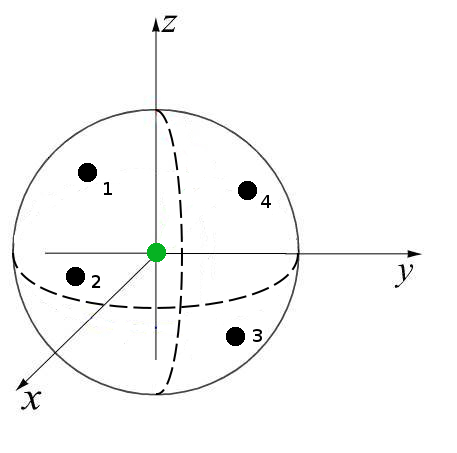
\includegraphics[scale=0.7]{figures/m11_spherexyz}\caption{Visualization of pixels taken to interpolate}
\label{fig:figures/m11_spherexyz } 
\end{figure}



\chapter{Implementation}

\input{"Implementation/Tools"}

\section{Module 1. MRI reconstruction}

Classical least squares estimation provides only the minimization of data error, which is an invalid solution. Conventionally, the LSE solution has a huge norm and thus it is a valueless outcome of a~reconstruction procedure. To this end, we introduced basic Tikhonov regularization method that seem to partially overcome the problem. However, we firstly implemented LSE approach for later usage of the results obtained with this procedure in restoration of the images from a~`nearby' well-posed problem (regularization). For Tikhonov regularization, additional quadratic penalty term allows controlling the norm of the solution, which benefits in introduction of smoothness prior to estimated solution. 

Firstly, we checked the data dimension that we load to the programme, as we could receive data starting from 3D to 5D. The implementation works for single slice structural and diffusion data (from many gradients) as well as for a whole set of brain slices. First two dimensions, provides information about data resolution i.e. $128\times 256$, which means that the images where subsampled with factor $r=2$. In case of structural data, the third dimension would be the number of slices (then, the forth is number of coils images) or simply number of coils images. For diffusion data, in 5D case the third dimension stands for number of slices, the forth - number of diffusion gradients and the fifth - number of coils images. The third dimension can be equal to one, so we get 4D data i.e. diffusion data for one slice. We also tested whether input dataset contains matrices with sensitivity maps profiles of a proper size, corresponding to maximal dimension of an image i.e. $256\times 256\times 8$, for case of images acquired with $8$ coils. Furthermore, the input files should also contain subsampling factor $r$ and number of coils $L$, if not, they can be calculated having the dataset's dimensional information.
 
Secondly, we performed 2D inverse Fourier Transform (2D IFT) on each of the dataset image, to transform them from \textbf{k}-space to \textbf{x}-space. This stage of an algorithm is presented in Fig. \ref{rys:subsampled}.  

\begin{figure}[h!]
\centering
  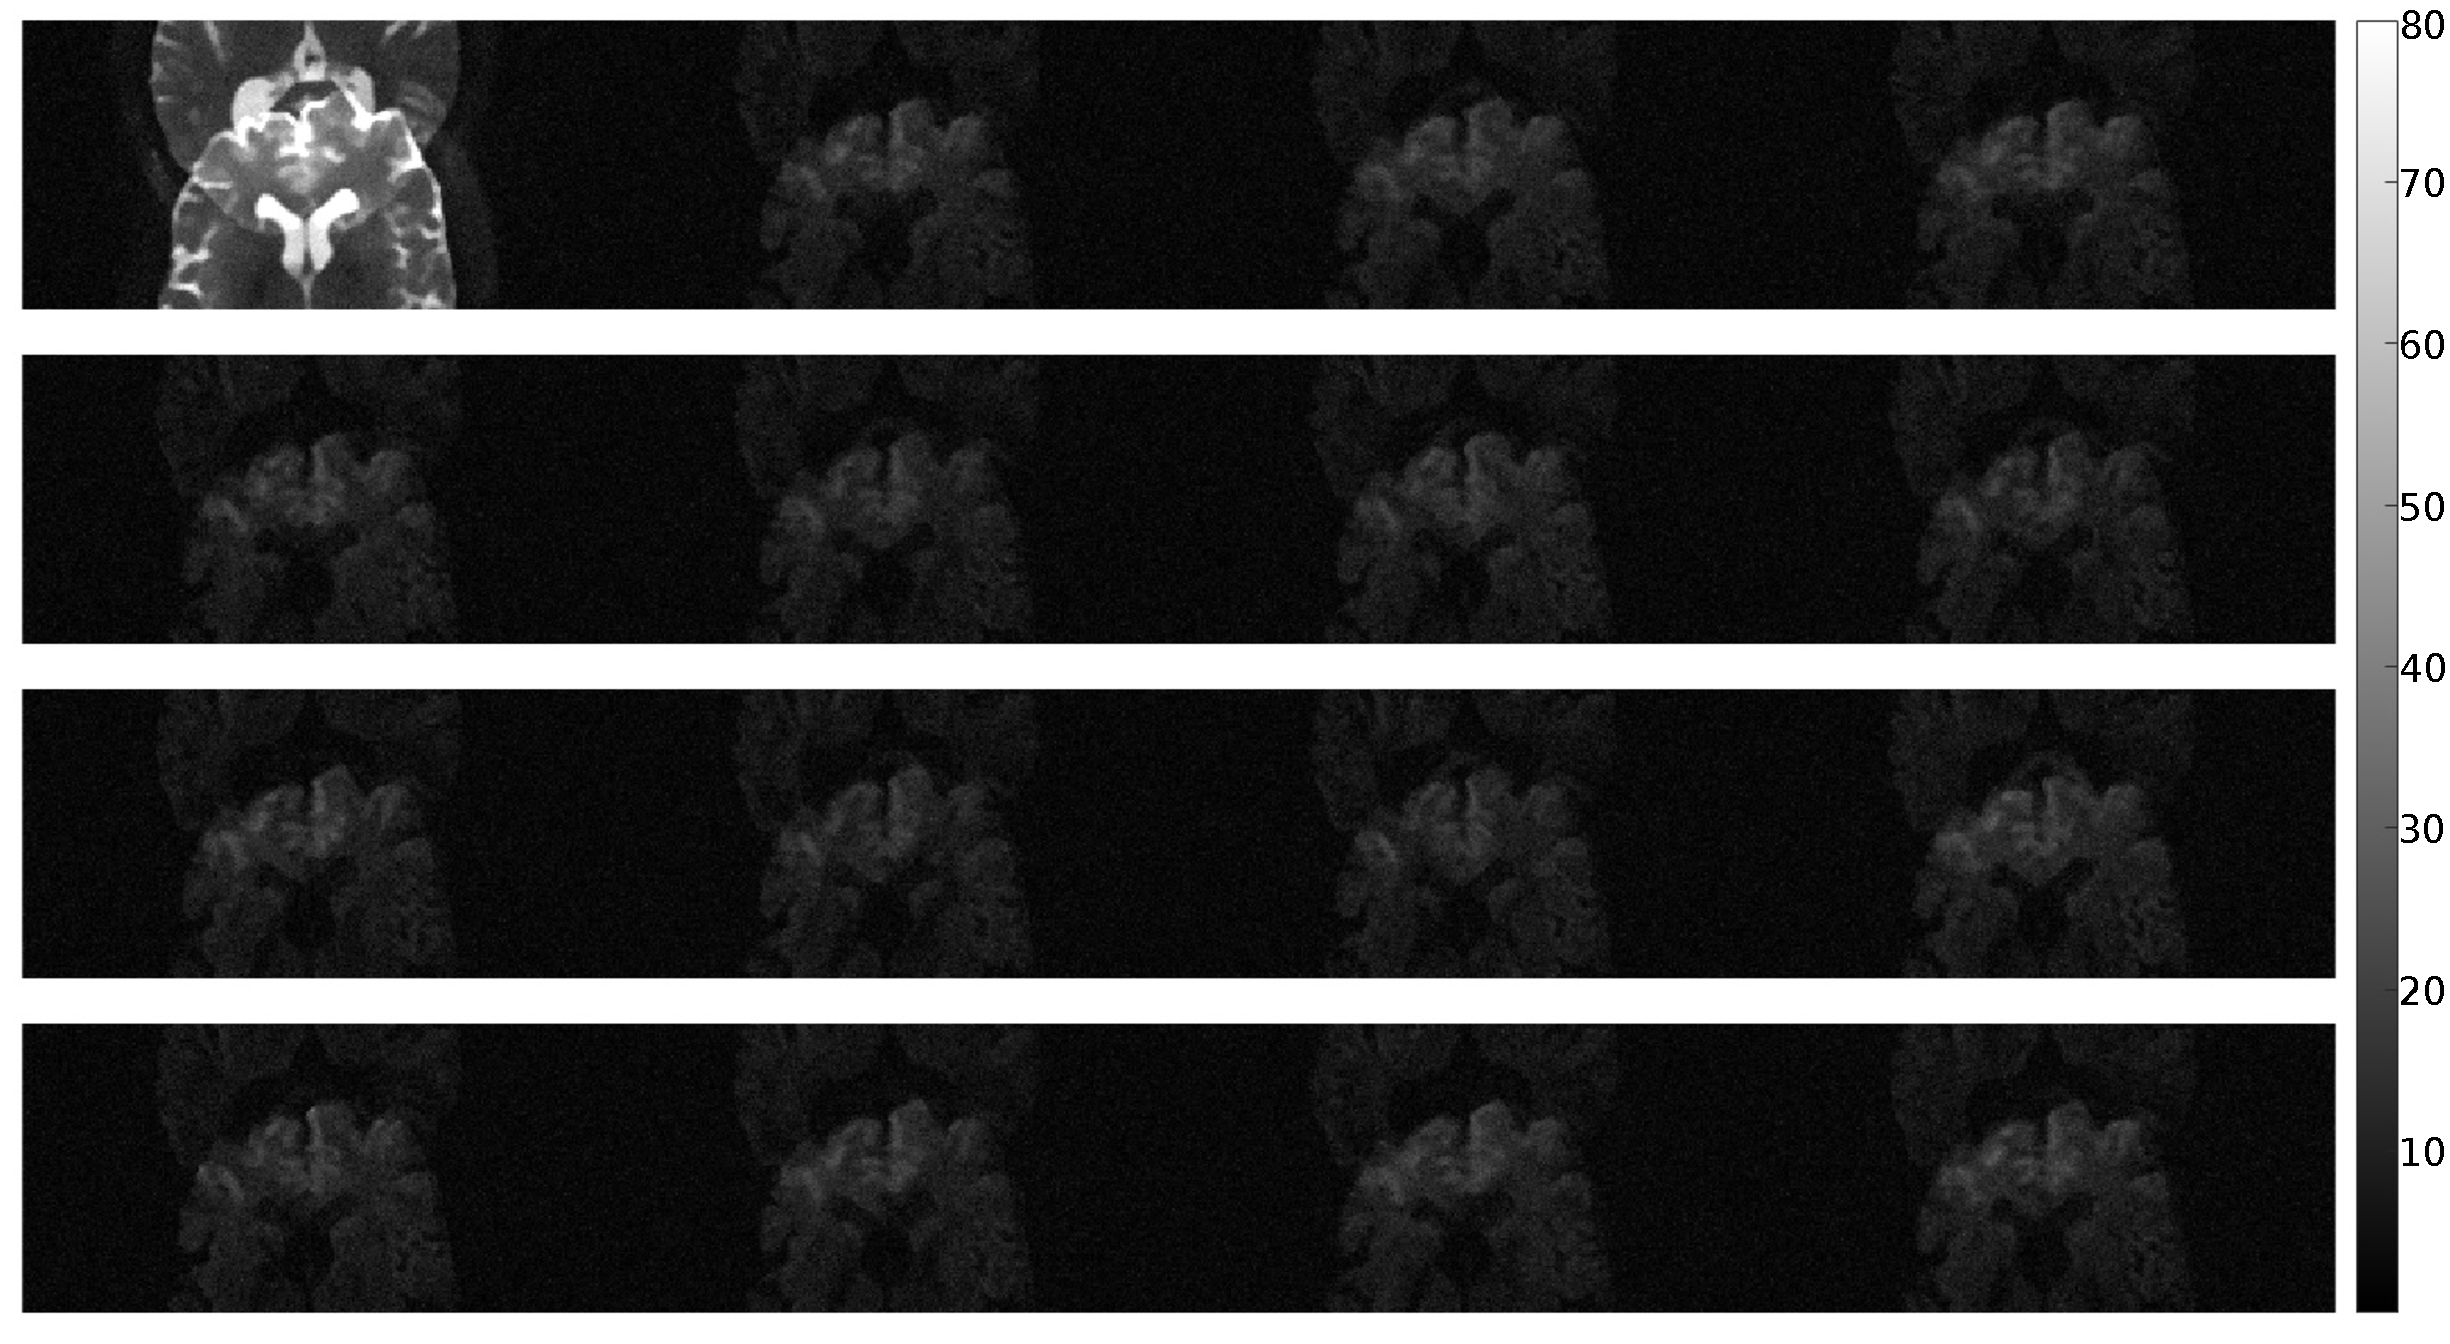
\includegraphics[scale=0.36]{figures/Module_01/NON_RECON.pdf}
  \caption{Subsampled diffusion dataset in \textbf{x}-space domain (data for one particular slice, acquired for 15 diffusion weightening gradients).}
  \label{rys:subsampled}
\end{figure}

\begin{figure}[h!]
\centering
  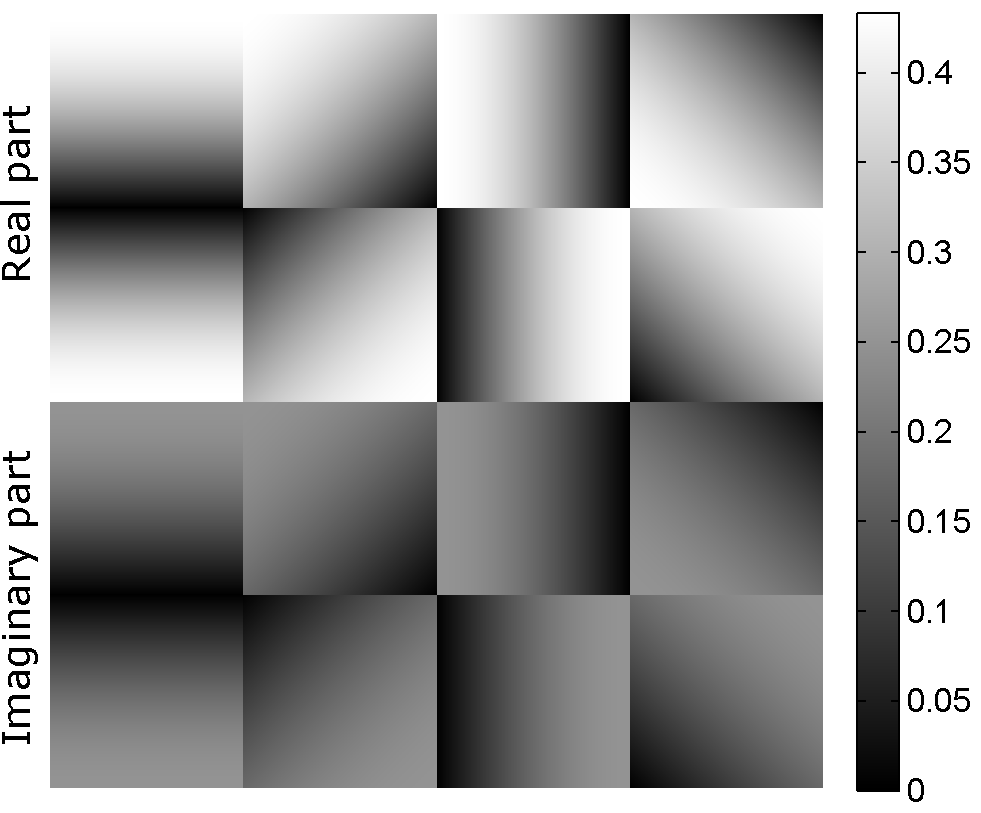
\includegraphics[scale=0.46]{figures/Module_01/MAPS.pdf}
  \caption{The real and imaginary parts of sensitivity maps used to reconstruct data ($L = 8$).}
  \label{rys:maps}
\end{figure}

\begin{figure}[h!]
\centering
  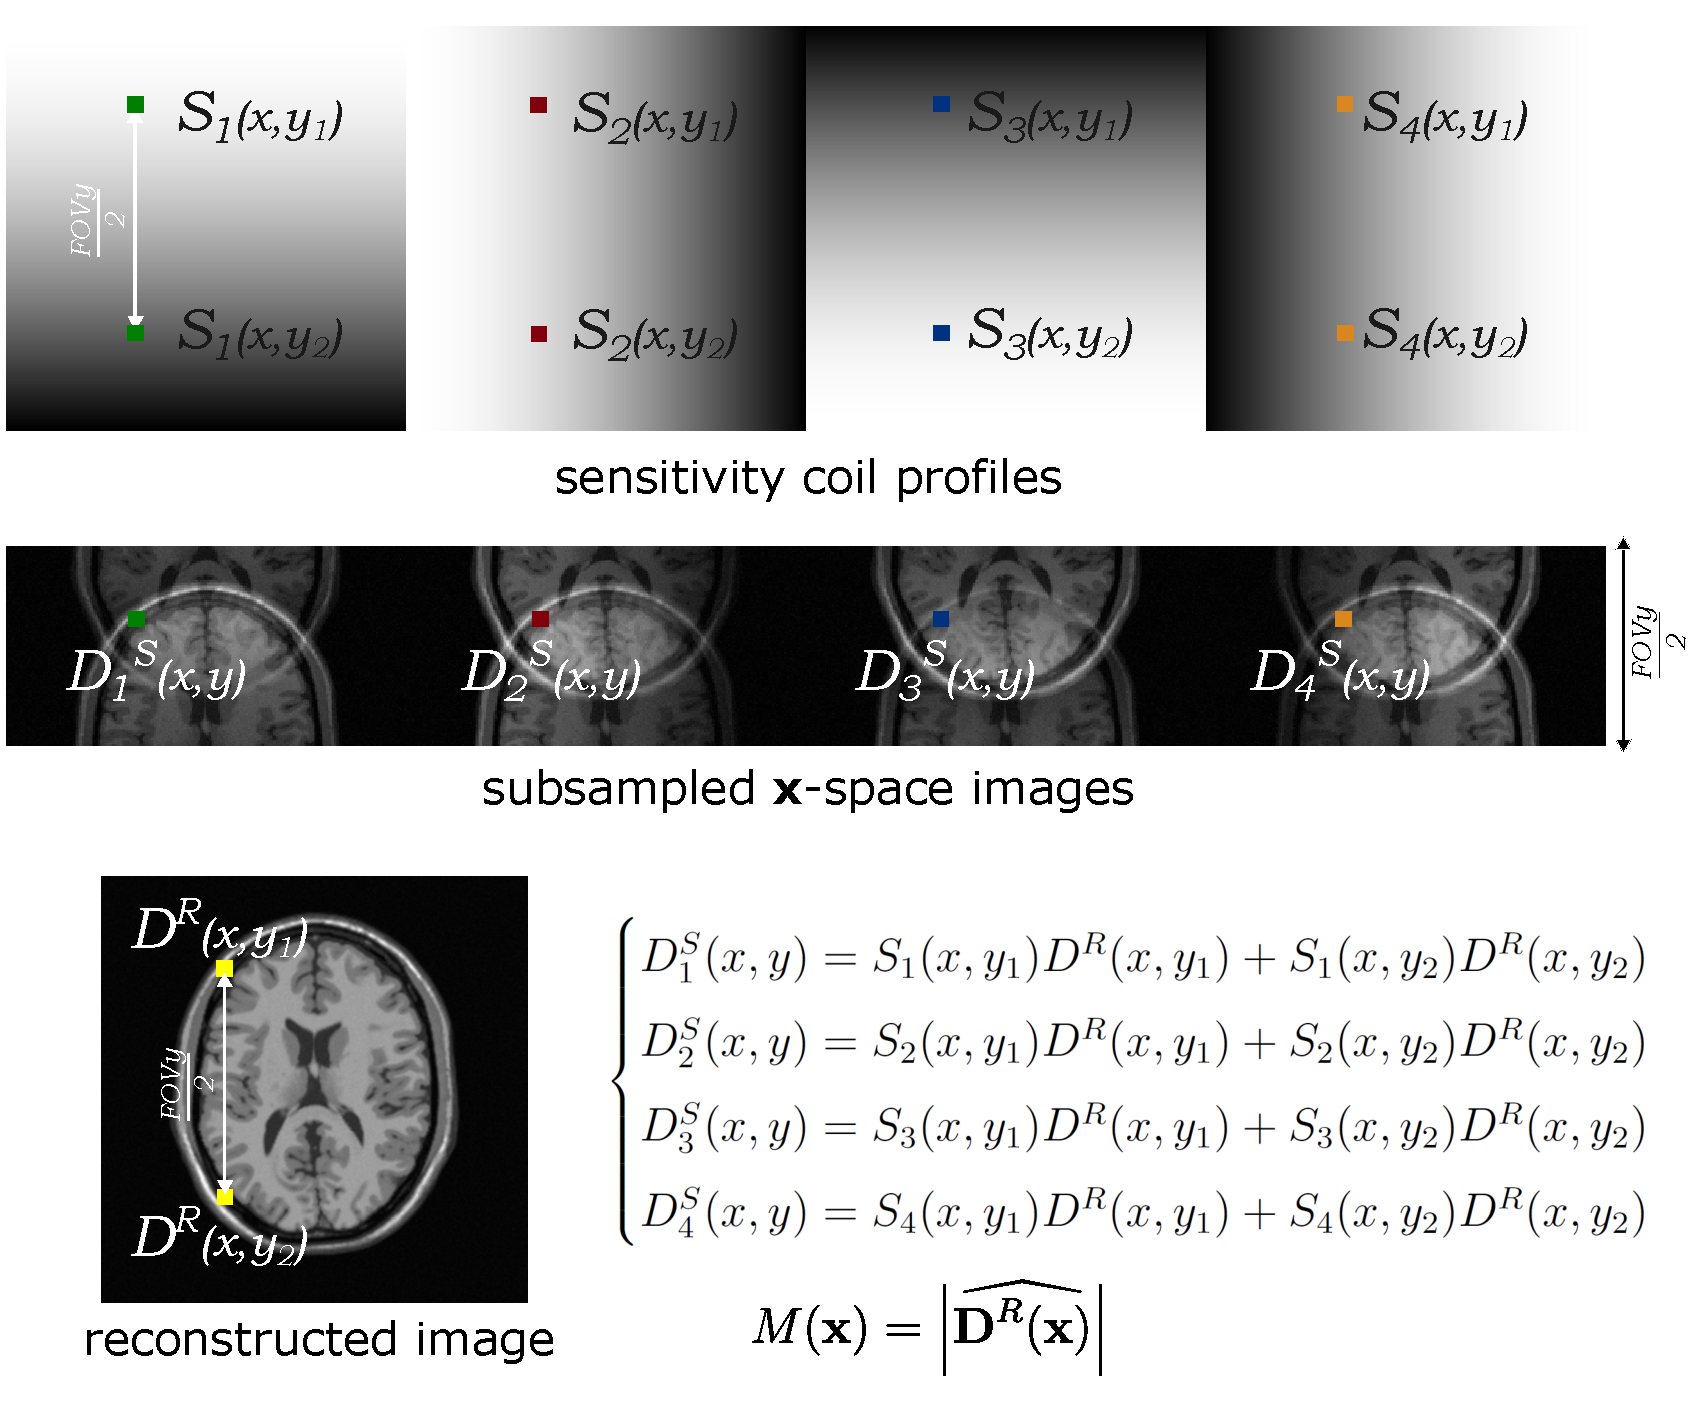
\includegraphics[scale=0.36]{figures/Module_01/SENSE.pdf}
  \caption{SENSE algorithm graphical explanation of Cartesian sampling using four receiver
coils ($L = 4$) and the subsampling rate $r = 2$. Two yellow pixels of the reconstructed image are
unfolded using coil sensitivity profiles and the corresponding folded pixels (points marked with
green, red, blue and orange).}
  \label{rys:sense}
\end{figure}

Thirdly, we used absolute value operator right before performing the SENSE reconstruction main step. As we are provided with sensitivity maps profiles (Fig. \ref{rys:maps}), we can easily reconstruct the subsampled data as it is shown in Fig. \ref{rys:sense}.
The key idea is to evaluate the algorithm pixel by pixel. According to equation \ref{Eq:wzor4}, the construction of defined $\textbf{D}^{S}$ vector is simple. Basically, the $\textbf{D}^{S}$ is a column vector of $L\times1$ size, containing pixels withdrawn from each $L$ coil image at specified spatial location. The matrix $\textbf{S}$ we construct in a~subsequent way: the $l-th$ row of $\textbf{D}^{S}$ contains values of the sensitivity maps profiles, corresponding to data position in a subsampled image and moved by a subsampled FOV value (i.e. for $r=4$, $FOV_{y} = 256/4 = 64$) $r-1$ times. As a result, depending on the number of coils and subsampling rate value, we obtained a matrix of $L\times r$ size. In LSE sense, the result of computation of  for defined $\textbf{D}^{S}$ and~$\textbf{S}$ is column vector $\textbf{D}^{R}$ ($r\times 1$ size). 

However, the LSE approach is not an optimal solution, so we implemented the regularization approach which uses the \textit{a priori} information of searched solution obtained with LSE algorithm. The images obtained after first reconstruction are median filtered with window size$3$x$3$. We introduced this additional information to the solution of derived objective function according to Eq. \ref{Eq:wzor7}. In this case, $\textbf{D}^{S}$ and~$\textbf{S}$ are constructed in the same manner as for LSE case, however we regularized the solution with $\lambda$ parameter. The choice of appropriate value of regularization parameter allows controlling the balance between both components (bias-variance tradeoff). For this scenario, we empirically picked $\lambda$ parameter as a constant value. As the reconstruction is performed pointwisely, we introduced extra information about expected result as a vector $\textbf{D}$ of $r$x$1$ size, containing pixels from reconstructed median filtered LSE images corresponding spatially to those to be reestimated with Tikhonov approach. The result is similar, i.e., we derived values of $r$ reconstructed points, which differ from those obtained with basic LSE approach. Fig. \ref{rys:recon} presents exemplary result of Tikhonov reconstruction algorithm implemented in the software. 

\begin{figure}[h!]
\centering
  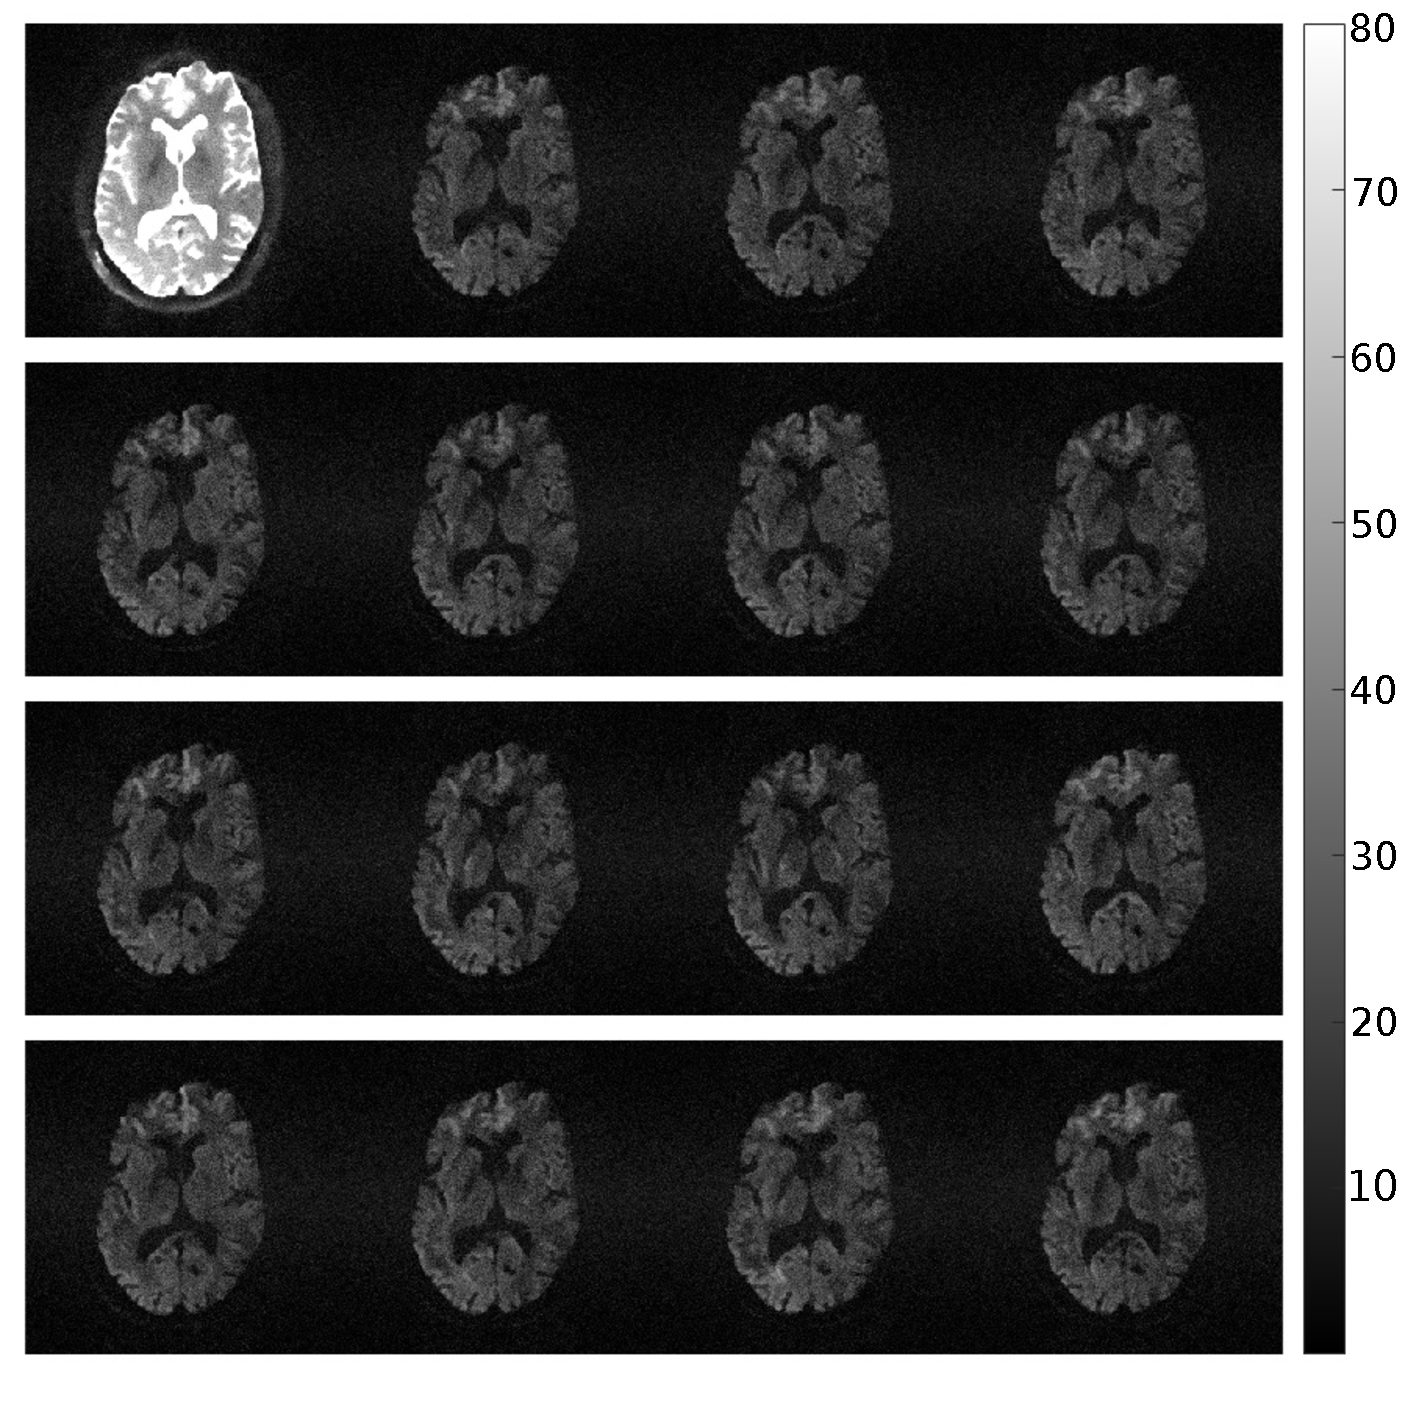
\includegraphics[scale=0.36]{figures/Module_01/RECON.pdf}
  \caption{Reconstructed diffusion dataset in \textbf{x}-space domain (data for one particular slice, acquired for 15 diffusion weightening gradients).}
  \label{rys:recon}
\end{figure}



\section{Module 2. Intensity inhomogeneity correction}

The Intensity inhomogeneity of the same tissue varies with the location
of the tissue within the image. In other words it refers to the slow,
nonanatomic intensity variations of the same tissue over the image
domain. It can be due to imaging instrumentation (such as radio-frequency
nonuniformity, static field inhomogeneity, etc.) or the patient movement.
This artifact is particularly severe in MR images captured by surface
coils. Although intensity inhomogeneity is usually hardly noticeable
to a human observer, many medical image analysis methods, such as
segmentation and registration, are highly sensitive to the spurious
variations of image intensities.

The aim of this module is estimation of intensity inhomogeneity field in MR image using surface fitting method. The method fits a parametric surface to a set of image features that contain information on intensity inhomogeneity. The resulting surface, which is usually polynomial or spline based, represents the multiplicative inhomogeneity field that is used to correct the input image.

The steps of this approach are: 
\begin{enumerate}
\item {Extract a background image from the corrupted MRI image, for example, by smoothing the image with a Gaussian filter of a large bandwidth (about 2/3 the size of the MRI image) to filter out all the image details that correspond to highfrequency components.}
\item {Select few data points from the background image and save their coordinates and graylevel values into a matrix $D = (xi , yi , gi), i = 1, 2, ...n$. It is recommended not to select points from the regions where there is no MRI signal since this regions has no bias field signal.}
\item {Select a parametric equation for the fitted surface . It is better to fit simple surfaces such as low order polynomial surfaces since they are very smooth and their parameters are very easy to estimate.}
\item {Estimate the parameters of the surface that best fits the data in matrix D by the method of nonlinear least-squares.}
\item {Use the fitted equation to generate an image of the bias field signal.}
\item {Divide the corrupted MRI image by the estimated bias field image in step 5.} 
\end{enumerate}
Even though different surfaces can reasonably fit the data very well and it is not possible to tell which surface is most likely represents the actual bias field signal, however, in practice the bias signal estimated by fitting a smooth 2-dimensional polynomial surface to a background image can be used effectively to restore the corrupted MRI image.

Fitting of the surface can be done by means of the Levenberg-Marquardt algorithm for nonlinear least squares fitting of a function $f(x, y; a_{1}, ..., a_{m})$ of known form to $n$ data points ${(x_{1}, y_{1}, g_{1}), ...,(xn, yn, gn)}$. For example, a polynomial surface of degree three can be fitted which has the following equation: $f(x, y; a) = a_{1}x^{3} + a_{2}y^{3} + a_{3}$, where $a = {a_{1}, a_{2}, a_{3}}$ is the parameter vector that define the surface. If we substitute the data points in the nonlinear function we get an overdetermined set of equations, i.e.,
\begin{equation}
\begin{Bmatrix}
g_{1} = f(x_{1}, y_{1}; a_{1}, a_{2}, ..., a_{m})\\ 
\cdot                                            \\
\cdot                                            \\ 
g_{n} = f(x_{n}, y_{n}; a_{1}, a_{2}, ..., a_{m})\\ 
\end{Bmatrix}
\end{equation}
These equations can be solved to obtain the unknown parameter vector $(a_{1}, a_{2}, ..., a_{m})$ by minimizing the sum of the squares of the differences between the data and the fitted function
\begin{equation}
\begin{aligned}
Q(\textbf{a})=\dfrac{1}{2} \sum_{i=1}^{n}(g_{i} - f(x_{i},y_{i}; a_{1},a_{2}, ...,a_{m}))^{2}
\label{fig: eq2_1}
\end{aligned}
\end{equation}
Let $r_{i}(\textbf{a}) = (g_{i} - f( x_{i}, y_{i}; a_{1}, a_{2}, ..., a_{m})$, which is the residual vector of point $i$, then equation \ref{fig: eq2_1} can be written as:
\begin{equation}
\begin{aligned}
Q(\textbf{a})=\dfrac{1}{2} \sum_{i=1}^{n}(r_{1}(\textbf{a}))^{2}
\label{fig: eq2_2}
\end{aligned}
\end{equation}
According to the Levenberg-Marquardt algorithm, eq.\ref{fig: eq2_2} can be solved iteratively to find the values of the parameters vector ($\textbf{a}$) starting from an initial estimate of the parameter vector $(\textbf{a}_{0})$ using:
\begin{equation}
\begin{aligned}
\textbf{a}_{i+1} = \textbf{a}_{i} - (H + \lambda diag[H])^{-1} \bigtriangledown Q(\textbf{a}_{i})
\label{fig: eq2_3}
\end{aligned}
\end{equation}
where $H$ and $\bigtriangledown$Q($\textbf{a}_{1}$) are Hessian matrix and the gradient of Eq. \ref{fig: eq2_2} both evaluated at $a_{i}$, $diag[H]$ is the diagonal elements of the Hessian matrix. At each iteration, the algorithm tests the value of the residual error  and adjusts $\lambda$ accordingly. \cite{2a1}

\section{Module 3. Non-stationary noise estimation}
In order to test effectiveness of implemented algorithm the results of it were compared to results of algorithm prepared to perforem calculatioans contained in \cite{aja2015spatially}. The algorithm for the article was implemented in Matlab.
\begin{figure}[H]
	\centering{}
		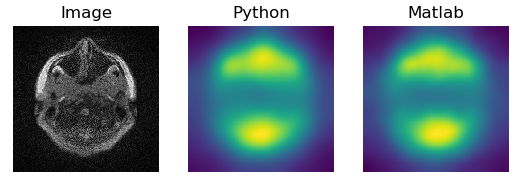
\includegraphics[scale=0.7]{figures/module03/10_comp}
	\caption{Image (left), noise map form Python algorithm(middle), noise map form Matlab algorithm(right).} 
\end{figure}
\begin{figure}[H]
	\centering{}
		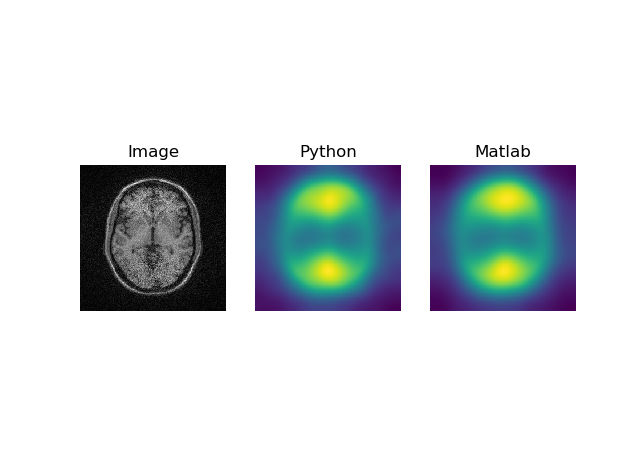
\includegraphics[scale=0.7]{figures/module03/70_comp}
	\caption{Image (left), noise map form Python algorithm(middle), noise map form Matlab algorithm(right).} 
\end{figure}
\begin{figure}[H]
	\centering{}
		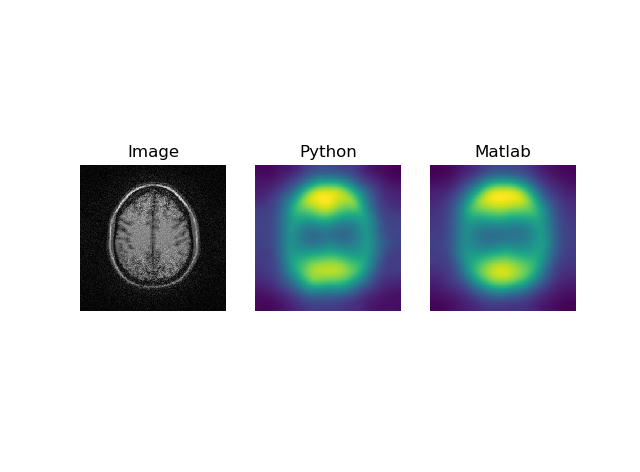
\includegraphics[scale=0.7]{figures/module03/110_comp}
	\caption{Image (left), noise map form Python algorithm(middle), noise map form Matlab algorithm(right).} 
\end{figure}
\begin{figure}[H]
	\centering{}
		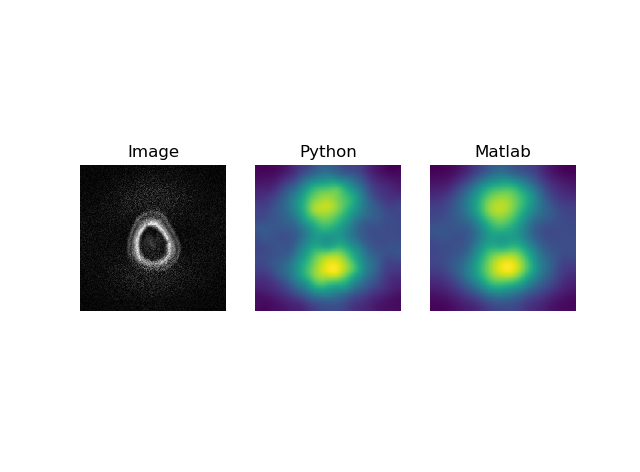
\includegraphics[scale=0.7]{figures/module03/160_comp}
	\caption{Image (left), noise map form Python algorithm(middle), noise map form Matlab algorithm(right).} 
\end{figure}
Results from Python algorithm are not perfect equivalent of the results from Matlab algorithm however ther are very similar and seem to be suitable for 
further processing of the image.

\section{Module 4. Non-stationary noise filtering 1}

The aim of this module is to remove Rician noise from MR images. If
both real and imaginary parts of signal are corrupted with zero-mean
uncorrelated Gaussian noise with equal variance, the envelope of magnitude
signal will follow a Rician distribution. Many processes allow to
remove noise, here the method is used to denoise MR images is the
linear minimum square error estimator (LMMSE). The main purpose of
LMMSE is to find a closed-form estimator for a signal that follows
a Rician distributions. It is more efficient than optimization-based
solutions. The estimator uses information of the sample distribution
of local statistics of the image such as the local mean, the local
variance and the local mean square value. In this method, the true
value for each noisy pixel is estimated by a set of pixels selected
from a local neighborhood.

The LMMSE estimator for a 2-D signal with Rician distribution is defined:

\begin{equation}
\begin{aligned}\widehat{A_{ij}^{2}}=E\{A_{ij}^{2}\}+C_{A_{ij}^{2}M_{ij}^{2}}C_{M_{ij}^{2}M_{ij}^{2}}^{-1}(M_{ij}^{2}-E\{M_{ij}^{2}\})\end{aligned}
\label{m4eq1}
\end{equation}
where $A_{ij}$ is the unknown intensity value in pixel $ij$, $M_{i}j$
the observation vector, $C_{A_{ij}^{2}M_{ij}^{2}}$ the cross-covarience
vector and $C_{M_{ij}^{2}M_{ij}^{2}}$ the covarience matrix. If the
estimator is simplified to be pointwise, vectors and matrics become
scalar values. Then the assuming local ergodicity with a square nighbourhood
around the pixel $ij$, the finally equation for LMMSE is defined:
\begin{equation}
\begin{aligned}\widehat{A_{ij}^{2}}=\langle M_{i}j^{2}\rangle-2\sigma_{n}^{2}+K_{ij}(M_{ij}^{2}-\langle M_{ij}^{2}\rangle)\end{aligned}
\label{m4eq2}
\end{equation}
with $K_{ij}$ 
\begin{equation}
\begin{aligned}K_{ij}^{2}=1-\frac{4\sigma_{n}^{2}(\langle M_{i}j^{2}\rangle-2\sigma_{n}^{2})}{\langle M_{i}j^{4}\rangle-{\langle M_{i}j^{2}\rangle}^{2}}\end{aligned}
\label{m4eq3}
\end{equation}

The LMMSE estimator is related to the quality of the estimate of the
noise variance $\sigma_{n}^{2}$. For the noise estimation the mode
of the sample mean is used:

\begin{equation}
\begin{aligned}\widehat{\sigma_{n}}=\sqrt{\frac{2}{\pi}}mode(\widehat{\mu_{1}}_{ij})\end{aligned}
\label{m4eq4}
\end{equation}
where $\widehat{\mu_{1}}_{ij}$ 
\begin{equation}
\begin{aligned}\widehat{\mu_{1}}_{ij}=\frac{1}{|\eta_{ij}}\sum_{p\colon\eta_{ij}}I_{p}\end{aligned}
\label{m4eq5}
\end{equation}

The use of the LMMSE method should makes the filtering process computationally
far more efficient and easier to implement. Also the use of local
statistics should decrease estimator dependent of parameters such
as the size of window.

\textbf{\emph{Module input}}: Reconstructed, normalized and corrected
data.

\textbf{\emph{Module output}}: Image without Rician noise.

\section{Module 5. Non-stationary noise filtering 2}

Magnetic Resonance images are endangered of being corrupted by noise
and artifacts. Since they are used as a basis for medical diagnosis
their quality has to be at highest possible level. Noise can be dealt
with by changing the parameters of images acquisition, however it
increases the scanning time, which is undesirable in medical imaging.
To overcome this obstacle, post-processing methods like filtering
are employed for denoising. In domain of MRI denoising many filters
may be used, though here emphasis is put on Unbiased Non-Local Means
(UNLM) filter, which is an extension of NLM filter. In order to understand
Unbiased version of this algorithm, the basic one has to be presented.

Having image \textit{Y}, the NLM algorithm calculates the new value
of point \textit{p} accordingly to the equation:

\begin{equation}
\begin{aligned}NLM(Y(p))=\sum_{\forall q\in Y}^ {}w(p,q)Y(q)\\
0\le w(p,q)\le1,\sum_{\forall q\in Y}^ {}w(p,q)=1
\end{aligned}
\label{m5e1}
\end{equation}

It can be seen that value of \textit{p} is calculated as weighted
average of pixels in the image (\textit{q}), having fulfilled restrictions
from \ref{m5e1}. To determine before mentioned average the similarity
between square neighbourhoods widows centered around pixels \textit{p}
and \textit{q} are calculated. The size of the window can determined
by the user, defined by parameter $R_{sim}$. Equation \ref{m5e2}
shows how to determine this similarity.

\begin{equation}
w(p,q)=\frac{1}{Z(p)}e^{\dfrac{d(p,q)}{h^{2}}}\label{m5e2}
\end{equation}

\textit{Z(p)} is the normalizing constant which also uses exponential
decay parameter \textit{h} and the weighted Euclidean distance measure
for pixels in each neighbourhood, called \textit{d}.

\begin{equation}
Z(p)=\sum_{\forall q}^ {}e^{\dfrac{d(p,q)}{h^{2}}}\label{m5e5}
\end{equation}

\begin{equation}
d(p,q)=G_{p}||Y(N_{p})-Y(N_{q})||_{R_{sim}}^{2}\label{m5e6}
\end{equation}

In above equation $G_{p}$ stands for a Gaussian weighting function
that has a 0 mean and standard deviation usually equal to 1.


Once NLM filter is fully explained, unbiased extension of it can be
examined. It builds on the properties of MRI signal. According to
\cite{5a1} the magnitude signal of MRI follows a Rician distribution.
Furthermore, for low intensity regions the Rician distribution approaches
to a Rayleigh one, whilst for high intensity it shifts towards Gaussian.
It was investigated that this bias can be handled by filtering the
squared MRI image, since it is not longer signal-dependent \cite{5a1}.
As a consequence the bias, which equals 2$\sigma^{2}$ \cite{5a3}
can be deleted with ease. The blueprint for UNLM can be summarized
in:
\begin{itemize}
\item noise estimation - which can be done by calculating standard deviation
of background in the image. To distinguish
background and the body on the MRI scan the Otsu thresholding method
\cite{5a4} can be successfully used. In this version noise maps are used, to achieve
non-stationary noise filtration, 
\item calculating NLM values for each point of image as in \ref{m5e1}, 
\item assessing the unbiased value of each point accordingly to the equation
\ref{m5e3}.
\end{itemize}
\begin{equation}
UNLM(Y)=\sqrt{NLM(Y)^{2}-2\sigma^{2}}\label{m5e3}
\end{equation}

In above equation $\sigma$ refers to value of non-stationary noise in the signal, more precisely
it is a value for each pixel from the original image, stored in a form of noise map.

% dwi, if it has to be joint implementation 
UNML implementation for diffusion weighted data becomes a bit less
trivial task, due to the new dimension of data associated with different gradients for each slice.
Based on assumption that gradients in similar directions
present related behaviours, UNLM for DWI can be formulated as:

\begin{equation}
Y_{i}(p)=\sqrt{\sum_{j\in\Theta_{i}^{N}}^ {}\sum_{q\in N_{p}}^ {}w_{i}^{j}(p,q)M_{j}^{2}(q)-2\sigma^{2}}
\end{equation}

Where weights are calculated as for structural data and \textit{M}
is a vector containing gray values.

\begin{equation}
d_{i}^{j}(p,q)=(M_{i}(N_{p})-M_{j}(N_{q}))^{T}G_{p}(M_{i}(N_{p})-M_{j}(N_{q}))\label{m5e7}
\end{equation}

However it was reported in \cite{5a2} that denoising diffusion weighted data using
UNLM method gives no significant results, so gradients related data can be ignored, or 
filtered as structural data.

It is worth mentioning that UNLM filter's performance is highly dependent
on parameter values. The optimal values of them were examined in \cite{5a1}
and same values are adapted in presented implementation. Properly-tuned
filter can significantly increase SNR of the scans while preserving
body structures.

\textbf{\emph{Module input}}: Previously reconstructed, normalized
and corrected data, noise maps.

\textbf{\emph{Module output}}: Image with deleted Rician noise by
unbiased non-local means filter. \\

\section{Module 6. Diffusion tensor imaging}

\textbf{Preprocessing and Module I/O}

In order to improve diffusion tensor estimation it is imperative to
remove artifacts. In addition to standard MRI pre-processing, one
needs to correct for artifacts arising the use of diffusion-gradient
pulse sequences and longer acquisition time. While hardware manufacturers
try to proactively diminish some of these effects, software processing
is still mandatory. 
\hfill\\

\textbf{Module Input}:
\begin{itemize}
	\item 
	3D structural data array of shape X x Y x Z, where XY - pixel image intensities, Z - chosen slice, which is the T1- or T2-weighted image corresponding the the given DWI acquisition
	
	\item 
	4D diffusion data array of shape X x Y x Z x M, where XY - pixel image intensities, Z - chosen slice, M - applied diffusion gradient direction
	
	\item 
	b\_value, a scalar value corresponding to applied diffusion gradient sequence magnitude
	
	\item 
	2D gradients matrix of shape M x 3, where each row corresponds to a normalized $(x,y,z)$ components of diffusion gradient sequence vectors
		
	\item 
	optionally - 3D binary mask of shape X x Y x Z, corresponding to the brain area detected by Module 8 (Skull Stripping); if not supplied, DTI is computed on each input data voxel

\end{itemize}
\hfill

\textbf{Module Output}:
\begin{itemize}
	\item
	list of size Z, corresponding to each slice; every list element is a dictionary of biomarker images: MD, RA, FA, VR of shape X x Y, and biomarker FA\_rgb of shape X x Y x 3
\end{itemize}

\subsection{Initialization}

In order to abstract DTI implementation from end-user, all classes and methods other than the main function \texttt{run\_module} are private to module source code script. It is important to note that prior to running the module one has to provide the module with input data object, as well as SOLVER and FIX\_METHOD parameters. SOLVER passed as an argument decides whether to use WLS or NLS estimation, whole FIX\_METHOD decides how to "fix" negative eigenvalues. 

As mentioned in the detailed description chapter, 'ABS' takes absolute value of each eigenvalue, while 'CHOLESKY' ensures that the estimated tensor is positive definite. Eigenvalues of positive definite matrices are always non-negative. 'ABS' is a post-estimation fix, meaning that it does not modify the default estimation algorithm (i.e. it is applied after WLS or NLS computation), while 'CHOLESKY' directly modifies the expressions for WLS and NLS cost function gradients and Hessian matrices.

After passing all required arguments to the \texttt{run\_module} function, they are reshaped internally in order to be compatible with module. Concretely, \texttt{DTISolver} class instance, computing the DTI proper, assumes that input data argument is a concatenated 3D array of both structural and diffusion images, which are stored separately in the original data structure. Moreover, b\_value and gradient fields are reshaped to be lists correpsonding to each slice of the new data array (that is: b\_value is repeated in length while both have zeros appended that correspond to structural images). Finally, all of the above is done separately for each slice and DTI module performs it's computation slice-by-slice due to memory constraints.

\subsection{WLS estimation}

WLS with the ABS fix method is a fast yet simple method of module pipeline computation based on diffusion tensor estimation. As such these parameters were set as default for DTI.

Diffusion tensor estimate was computed by implementing the equation:
\begin{equation}
\begin{aligned}
\boldsymbol{\gamma}=\left(\boldsymbol{W}^T\boldsymbol{\omega}^T\boldsymbol{\omega}\boldsymbol{W}\right)^{-1}\boldsymbol{W}^T\boldsymbol{\omega}^T\boldsymbol{\omega y}
\end{aligned}
\label{Eq:m6_impl_eq_1}
\end{equation}

using NumPy matrix broadcasting operations, effectively abstracting away array reshaping. Weights vector $\boldsymbol{\omega}$ is calculated using a separate function in order to avoid changing every piece of code refering to WLS weights in case they change. The following implementation assumes the simplest of models presented in the Detail Description chapter, that is weights being equal to the measured signal.

\subsection{NLS estimation}

In case of NLS estimation, in addition to implementing gradient and Hessian matrix computation methods:

\begin{equation}
\begin{aligned}
\nabla{f_{NLS}}&=-\boldsymbol{W}^T\boldsymbol{\hat{S}}\boldsymbol{r} \\
\nabla^2{f_{NLS}}&=\boldsymbol{W}^T\left(\boldsymbol{\hat{S}^T\hat{S}-\boldsymbol{R\hat{S}}}\right)\boldsymbol{W}
\end{aligned}
\label{Eq:m6_impl_2}
\end{equation}

It is important to devise an iterative scheme because gradient result depends on NLS diffusion tensor estimate. For that reason an algorithm based on \cite{m6_koay2006a} has been implemented. The method itself is called a Modified Newton's Algorithm and can be summarised as in Fig.\ref{fig:m6_pic_1}.

\begin{figure}[H]
	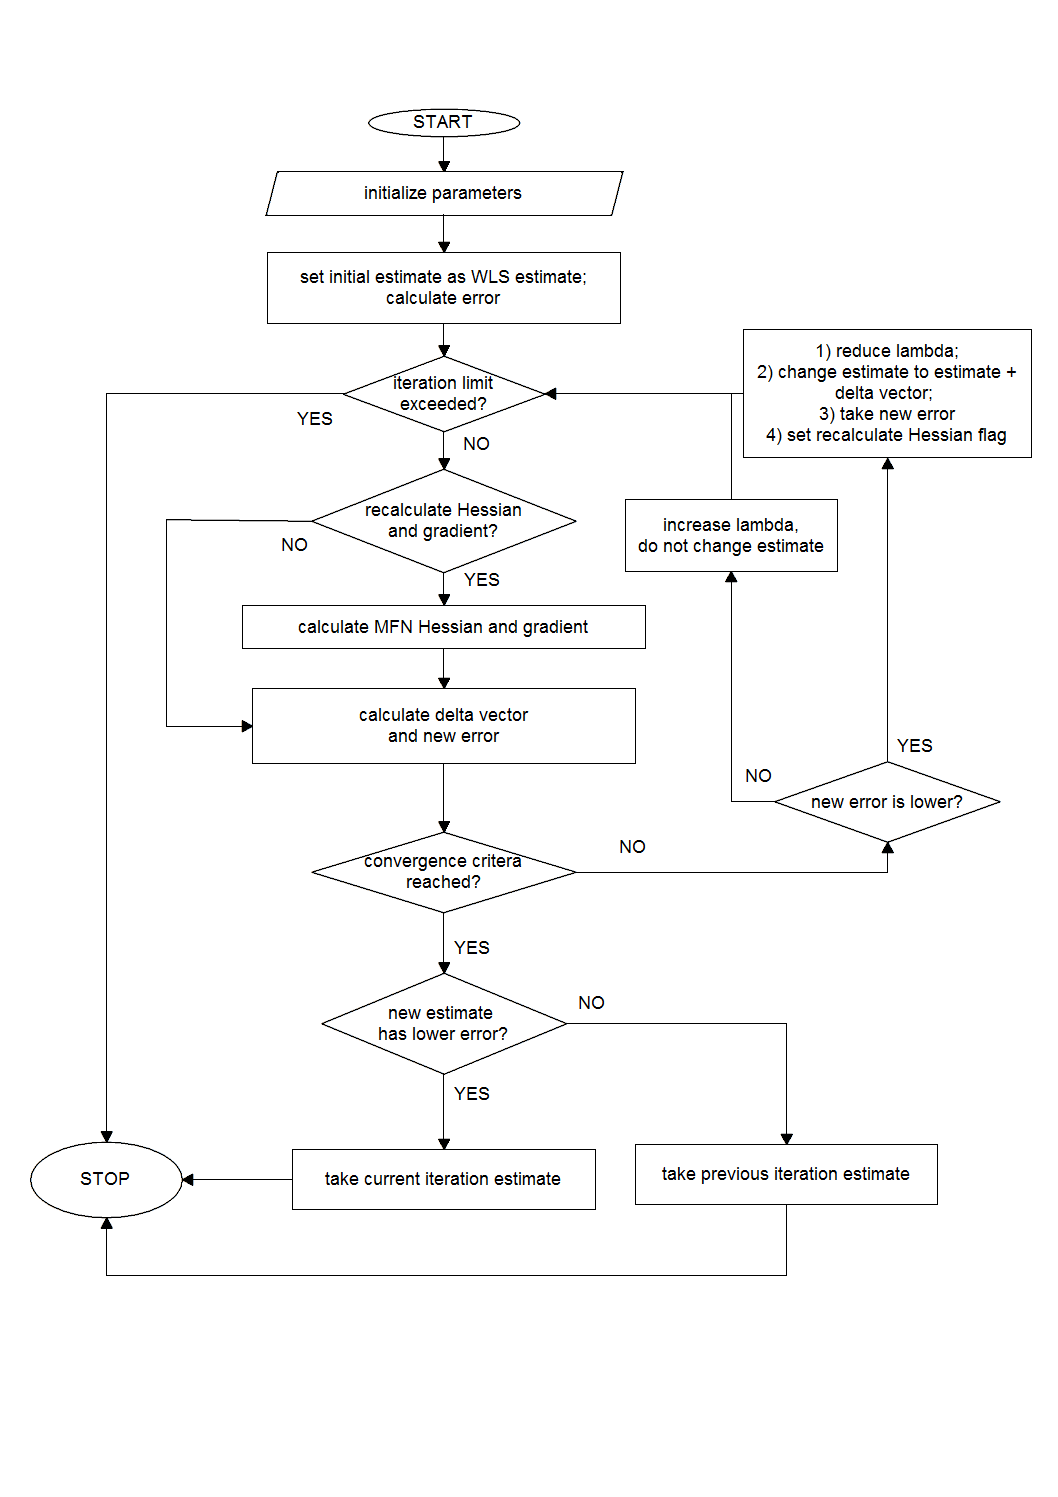
\includegraphics[width=8cm]{figures/Module_06/mfn_simple}
	\centering
	\caption{Modified Newton's method for iterative computation of NLS estimate \vbox{(based on \cite{m6_koay2006a})}}.
	\label{fig:m6_pic_1}
\end{figure}

The following parameters (collectively known in code as MFN parameters) were set:
\begin{itemize}
	\item 
	MFN\_MAX\_ITER = 3 - iteration limit
	
	\item
	MFN\_ERROR\_EPSILON = 1e-5 - first convergence criterion (error change is small)
	
	\item
	MFN\_GRADIENT\_EPSILON = 1e-5 - second convergence criterion (vanishing gradient)
	
	\item
	MFN\_LAMBDA\_MATRIX\_FUN = 'identity'- regularization matrix added to Hessian matrix
	
	\item 
	MFN\_LAMBDA\_PARAM\_INIT = 1e-4 - initial regularization matrix multiplier
\end{itemize}

Delta estimate is calculated using the following formula:
\begin{equation}
\boldsymbol{\delta}=-\left(\nabla^2{f_{NLS}+\lambda I}\right)^{-1}\nabla{f_{NLS}}
\label{Eq:m6_impl_3}
\end{equation}

with $\lambda$ parameter increasing and decreasing by a factor of 10, depending on whether newly calculated estimate yields lower error (decreasing for lower error, increasing otherwise).

Convergence is established using the following formulas:
\begin{equation}
\begin{aligned}
\left|f_{NLS_{new}} - f_{NLS_{new}}\right| &< \texttt{MFN\_ERROR\_EPSILON} \\
\delta^T\nabla{f_{NLS}} &< \texttt{MFN\_GRADIENT\_EPSILON}
\end{aligned}
\end{equation}

\subsection{Biomarkers computation}

As mentioned previously, the estimate obtained from NLS or WLS methods can be reshaped to a 3x3 matrix:
\begin{equation}
\boldsymbol{D}=
\begin{bmatrix}
D_{xx} & D_{xy} & D_{xz} \\
D_{yx} & D_{yy} & D_{yz} \\
D_{zx} & D_{zy} & D_{zz} 
\end{bmatrix}
\label{Eq:m6_impl_4}
\end{equation}
assuming our estimate is equivalent to:
\begin{equation}
\boldsymbol{\gamma}={\lbrack ln{S_0}, D_{xx}, D_{yy}, D_{zz}, D_{xy}, D_{yx}, D_{xz}\rbrack}^T
\label{Eq:m6_impl_5}
\end{equation}

Tensor estimation results for a sample 126x126x55 slice are presented on Fig.\ref{fig:m6_pic_2}.

\begin{figure}[H]
	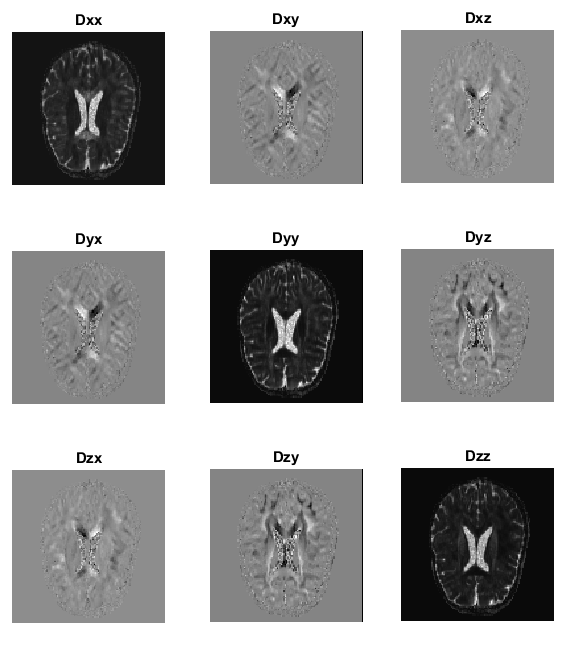
\includegraphics[width=16cm]{figures/Module_06/tensor_image}
	\centering
	\caption{Diffusion tensor estimate using the WLS-ABS method for a 126x126x55 test image.}
	\label{fig:m6_pic_2}
\end{figure}

We can then compute the eigenvalue decomposition of $\boldsymbol{D}$ and obtain eigenvalues and eigenvectors for each pixel of input image. Eigenvalues are sorted in descending order and saved for later computation (Fig.\ref{fig:m6_pic_3}). Moreover, eigenvectors corresponding to the highest eigenvalue are saved to separate variable, since they represent the direction of principal diffusion.

\begin{figure}[H]
	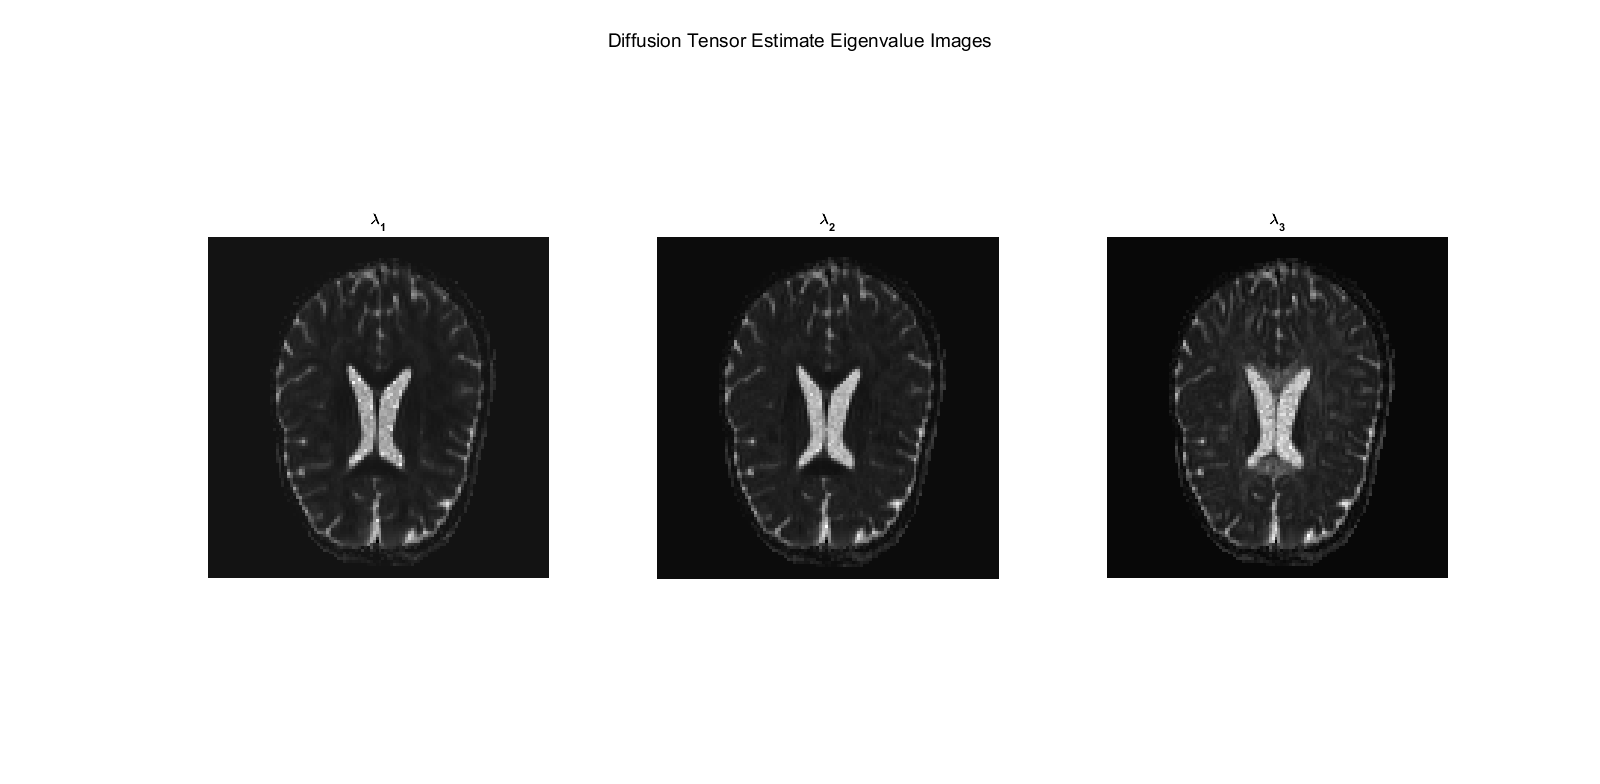
\includegraphics[width=16cm]{figures/Module_06/eig_image}
	\centering
	\caption{Diffusion tensor estimate eigenvalues of sample imgae; eigenvalues sorted in descending order from left to right.}
	\label{fig:m6_pic_3}
\end{figure}

Biomarkers are then computed using the following formulas:
\begin{equation}
MD = \dfrac{\lambda_{1}+\lambda_{2}+\lambda_{3}}{3}
\end{equation}
\begin{equation}
RA = \sqrt{\dfrac{\left(\lambda_{1}-MD\right)^2+\left(\lambda_{2}-MD\right)^2+\left(\lambda_{3}-MD\right)^2}{3\,MD}}
\end{equation}
\begin{equation}
FA = \sqrt{\dfrac{3}{2}}\sqrt{\dfrac{\left(\lambda_{1}-MD\right)^2+\left(\lambda_{2}-MD\right)^2+\left(\lambda_{3}-MD\right)^2}{\lambda_{1}^2+\lambda_{2}^2+\lambda_{3}^2}}
\end{equation}
\begin{equation}
VR = \frac{\lambda_{1}\lambda_{2}\lambda_{3}}{MD\,^3}
\end{equation}

Computed biomarkers of the sample image are presented on Fig.\ref{fig:m6_pic_4}. It is important to note that skull is visible because the brain area was selected by hand instead of relying on Module 08 output.

\begin{figure}[H]
	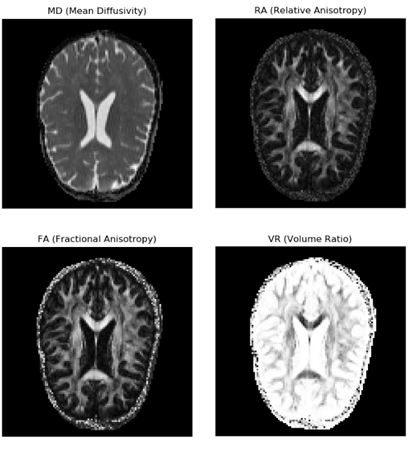
\includegraphics[width=12cm]{figures/Module_06/biomarkers_wls}
	\centering
	\caption{Diffusion biomarkers of sample image. Top left: MD, top right: RA, bottom left: FA, bottom right: VR.}
	\label{fig:m6_pic_4}
\end{figure}

Figure \ref{fig:m6_pic_5} presents the fifth biomarker image present in output dictionary - FA-weighted principal direction of diffusion color map. Color-encoded direction for this slice is presented as follows:
\begin{itemize}
	\item 
	red - transversal (left-right)
	
	\item 
	green - anterior-posterior (front-back)
	
	\item
	blue - cranio-caudal (head-feet)
\end{itemize}

\begin{figure}[H]
	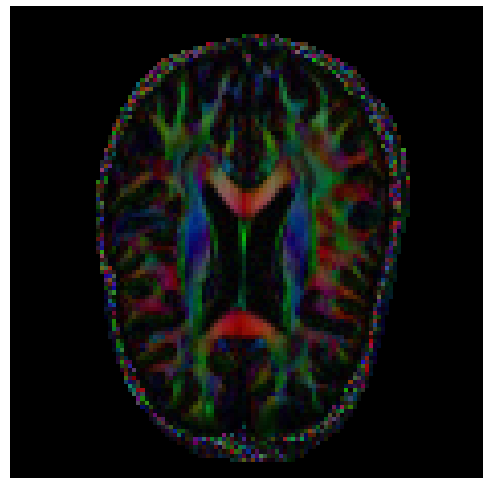
\includegraphics[width=10cm]{figures/Module_06/fa_rgb}
	\centering
	\caption{FA-weighted principal direction of diffusion of sample image.}
	\label{fig:m6_pic_5}
\end{figure}

\subsection{Implementation caveats}

Module source code was implemented and tested on a single sample image outlined above. It constituted a perfect basis for algorithm evaluation because it was already preprocessed, without the need to wait for other modules implementation. Even though it lacked a skull stripping mask, hand-drawn shape was good enough for testing, even though skull outline is visibly present, particularily on Fig.\ref{fig:m6_pic_5}. 

It was difficult to determine which estimation method - WLS or NLS - is objectively better. WLS was significantly faster and it was not much different from NLS results. This might have been due to the fact, that the diffusion-encoding gradient matrix was unusually large (7 structural images and 48 DWIs). Testing on preprocessed raw data, supplied for application evaluation has shown differences between methods, although both estimates are valid (to the Author's best knowledge) as it is difficult to compare any estimation methods without reference.

Initially developed using nested for-loops, DTI module has been vectorized to speed up computations. For a supplied 256x256x16 DWI stack a single slice is being processed in less than 3 seconds for WLS-ABS, while other methods scale linearily with chosen number of iterations (starting at 6 seconds, then 3 seconds per MFN iteration). It must be noted that the module was not tested with skull stripping mask, which could have drastically reduced computation time. Moreover computation time heavily depends on hardware constraints.

\section{Module 8. Skull stripping}

Preliminary processing to isolate the brain form extra-cranial or non-brain tissues such as e.g. the eye sockets, skin from MRI head scans is commonly referred as skull stripping. Skull stripping methods which are available in the literature are broadly classified into five categories: mathematical morphology-based metods, intensity-based methods, deformable surface-based methods, atlas-based methods, and hybrid methods. Each skull stripping method has their own merits and limitations.
The aim of this module is to remove pieces of skull from MRI Image using at pleasure chosen algorithm from the literature. Skull stripping is performed with use of two methods:
\begin{itemize}
    \item {Brain Surface Extractor BSE proposed by Stattuck et al. [1]}
    \item {Marker-controlled watershed algorithm by Abdallah and Hassan and by Segonne et al. [2], [3]}
\end{itemize}
Before this methods, there is applying preprocessing function to estimate global parameters: CSF - an upper bound for the intensity of the cerebrospinal fluid, COG - the coordinates of the centroid of the brain, BR - the average brain radius and ratio to brain diameter in axis x to brain radius in axis y. These estimated parameters are useful in this to methods to optimization and working.
BSE procedure consist of three steps:
\begin{enumerate}
\item {The MRI is processed with anisotropic diffusion filter to smooth nonessential gradients.}
\item {The filtered image has applied a Marr-Hildreth edge detector to identify important anatomical boundaries.}
\item {Using a sequence of morphological and connect component operation to define object by previous boundaries.}
\end{enumerate}

Anisotropic Diffusion filtering is applied to smooth noisy regions, which can obscure boundaries or their edges can be indistinguishable from the other in the image. To implement this filter is used an image processing method by Perona and Malik. They demonstrated that using the gradient of image intensity as an estimate of edge strength produces good results. The filtered image is modeled as the solution to the anisotropic diffusion equation
\begin{equation}
    \frac{\partial I}{\partial t} = \nabla \cdot (c(\textbf{p},t)\nabla I) = c(\textbf{p},t)\nabla^{2}I + \nabla c \cdot \nabla I  \label{Eq:wzor_1}
\end{equation}
where \textbf{p} is a point in $R^{2}$, $\nabla$ and $\nabla^{2}$  represent the gradient and Laplacian operators and $\nabla$ $\cdot$ indicates the divergence operator. The function is defined as:
\begin{equation}
    c(\textbf{p},t) = g(\parallel\nabla I(\boldsymbol{p},t)\parallel) = e^{-\parallel\nabla I(\textbf{p},t)\parallel^{2} \kappa^{2}_{d}} \label{Eq:wzor_2}
\end{equation}
where $\kappa_{d}$ is the diffusion constant. \eqref{Eq:wzor_2} gives preferences to high-contrast edges. Number of iteration and the diffusion parameter $\kappa_{d}$ is selected empirically.

To locate the anatomical boundaries in MRI brain volumes, it is used the Marr-Hildreth edge detectors. It is based on a low-pass filtering step with a symetric Gaussian kernel, followed by the localization of zero-crossing in the Laplacian of the filtered image. The Marr-Hildreth operator is defined as:
\begin{equation}
    C(k) = \nabla^{2}(I(k)*g_{\sigma}(\textbf{p})) \label{Eq:wzor_3}
\end{equation}
where C is the output contour image, I is an input image, * is the convolution operator, $g_{\sigma}$ is a Gaussian kernel with variance $\sigma^{2}$
\begin{equation}
    g_{\sigma} = \frac{1}{\sqrt{2\pi}\sigma}e^{- \parallel\textbf{p}\parallel^{2}/2\sigma^{2}} \label{Eq:wzor_4}
\end{equation}
where \textbf{p} is a point in the image, and $\nabla^{2}$ is the Laplacian operator.
To find pixels in the contour image, C where zerocrossing occur, a binary image E is produced that separates the image into edge-differentiated segments. Small values for sigma produce narrow filters, resulting in more edges in the image, on the other hand increasing this value makes the blurring kernel wider and only strong edges remain. This detector output is an image, which edge pixels are black and nonedge ones are white.

Morphological processing’s task is to select the pixels corresponding to the brain tissue from the original image. The output of edge detector often does not distinguish meninges or blood vessels from the brain tissue due to noise, low contrast between brain and meninges or true anatomical continuity. The first step is morphological erosion, which delete narrow connections without globally damaging image. After that the largest connected region centered in the volume consist entirely of brain tissue. Second step is selection of this region. Third step, is binary dilatation to restore the brain due to previous erosion, which decrease brain surface. Because of imperfections in the edge boundaries detection, image after dilatation may consist of pits in its surface or small holes within the surface. The last step of morphological processing is closing, which fill small pits and close of some holes that occur.

Marker-controlled watershed segmentation follows this procedure:
\begin{enumerate}
    \item {Computation a segmentation function.}
    \item {Computation the foreground markers.}
    \item {Computation the background markers.}
    \item {Computation of the watershed transform using of the foreground markers and the background markers.}
\end{enumerate}
First step is applied to find the edges in the image, it is processed with Sobel edge filter. The gradient is high at the borders of the object and low inside. Morphological techniques are used to compute the foreground markers, opening by reconstruction and closing by reconstruction to clean up the image. These operation will create flat regional maxima inside each object that can be used to find regional maxima and next modified them by a closing followed by an erosion to obtain good foreground markers. The background pixels after binarization are black, but their markers should be to close to the edges of the object. this can by done by computing the watershed transform of the distance transform of the binary image and the looking for the watershed ridges lines of the result. With the foreground markers and the background markers there is applied watershed based segmentation.

Brain Surface Extraction and Marker-controlled Watershed Segmentation is working separately. The base method is BSE. Marker-controlled watershed segmentation is compute, when BSE brain mask is larger than a mask based on preprocessing estimated BR.

\hfill{}\\
\textbf{List of References}\\
\cite{8_dti_1}, \cite{8_dti_2}, \cite{8_dti_3}, \cite{8_dti_4},


\section{Module 9. Segmentation}

Brain MRI segmentation is an essential task in many clinical applications
because it influences the entire analysis. This is because different
processing steps rely on accurate segmentation of anatomical regions.
For example, MRI segmentation is commonly used for measuring and visualizing
different brain structures, for delineating lesions, for analysing
brain development, and for image-guided interventions and surgical
planning.

\textit{MRI Processing} To prepare brain MRI for segmentation, it
is necessary to perform several preprocessing steps. (Fig. \ref{fig:Preprocessing}).

\begin{figure}[H]
\centering{}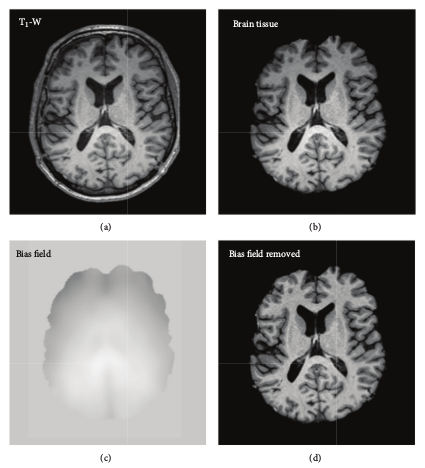
\includegraphics[scale=0.7,bb = 0 0 200 100, draft, type=eps]{9Preprocessing}\caption{Triangulation for the 15 patterns. \label{fig:Preprocessing}}
\end{figure}

The most important steps are: MRI bias field correction, image registration
and brain extraction.

\textit{Basic} An image for segmentation can be defined in 2D space
(pixels) or in 3D space (voxels). Each image element is specified
by its intensity value and coordinates for pixels (i,j) and for voxels
(i,j,k). Intensity values are typically represented by a gray value
{0, …, 255}.

The goal of image segmentation is to divide an image into a set of
semantically meaningful, homogeneous, and nonoverlapping regions of
similar attributes such as intensity, depth, color, or texture. Thesegmentation
result is either an image of labels identifying each homogeneous region
or a set of contours which describe the region boundaries.

Fundamental components of structural brain MRI analysis include the
classification of MRI data into specific tissue types and the identification
and description of specific anatomical structures. The problems of
segmentation and classification are interlinked because segmentation
implies a classification, while a classifier implicitly segments an
image. In the case of brain MRI, image elements are typically classified
into three main tissue types: white matter (WM), gray matter (GM),
and cerebrospinal fluid (CSF) (Fig. \ref{fig:Segment}).

\begin{figure}[H]
\centering{}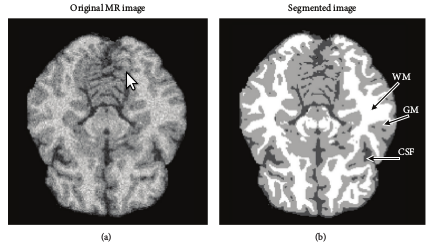
\includegraphics[scale=0.7,bb = 0 0 200 100, draft, type=eps]{9Segmentation}\caption{Triangulation for the 15 patterns. \label{fig:Segment}}
\end{figure}

One of the most important features for brain MRI segmentation is the
intensity of brain tissue. However, intensity-based segmentation algorithms
will lead to wrong results when intensity value are corrupted by MRI
artifacts.

\textit{MRI Segmentation Methods} There is no single method that can
be suitable for all images, nor are all methods equally good for a
particular type of image. For example, some of the methods use only
the gray level histogram, while some integrate spatial image information
to be robust for noisy environments. Some methods use probabilistic
or fuzzy set theoretic approaches, while some additionally integrate
prior knowledge (specific image formation model, e.g., MRI brain atlas)
to further improve segmentation performance. The segmentation methods,
with application to brain MRI, may be grouped as follows: 
\begin{itemize}
\item manual segmentation; 
\item intensity-based methods (including thresholding, region growing, classification,
and clustering); 
\item atlas-based methods; 
\item surface-based methods (including active contours and surfaces, and
multiphase active contours); 
\item hybrid segmentation methods. 
\end{itemize}
\hfill{}\\
\textbf{List of References}\\
\cite{09a1}

\section{Module 10. Upsampling}

The implementation began with making a decision about the input data. The input image has to be 2 dimensional without a noise. The uploaded image will be considered as a 2 dimensional array of double values. Other parameters that will be needed are vertical and horizontal extensions. It has to be a total number. The size of the input array will be multiplied by the number. For example, the image 256x256 pixels with extensions equal to 3 will be 768x768 pixels as an output. The function needs also the window size. In one iteration, the function will take into consideration only pixels witch are inside the window. The loop will stop only when the whole image will be interpolated. To see the results the \textit{plotting} parameter has to be a boolean \textit{True} value. 
\newline The below picture shows the block diagram of the algorithm (Fig. \ref{fig: Module10_4}) with comments added.

\begin{figure}[H]
\centering{}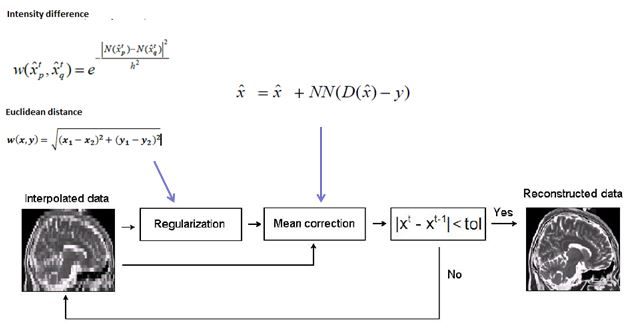
\includegraphics[scale=0.7]{figures/Module_10/Module10_4}\caption{Algorithm block diagram with comments}. 
\label{fig: Module10_4}
\end{figure}

The following steps of the implementation will be discussed:

\begin{enumerate}

\item \textbf{Initial interpolation}
\newline To form the input image into the output with chosen size the initial interpolation is needed. As showed in \cite{9art1} the spline interpolation is used. In short, spline interpolation is an interpolation where interpolant is a special kind of piecewise polynomial called spline. It is recommended, because of the fact that the method makes small error even with low degree polynomials for the spline. Taking into consideration the edges the extrapolation was applied. To be more specific, the last row \textit{n} is equal to the previous one \textit{n-1}. The same with the first row, the first column and the last column of the input. To show the results, the extensions are set as 2. The input data is 256x256 pixels. The undermentioned picture (Fig. \ref{fig: Module10_5}) shows the result of the initial interpolation. The scale is included so it is easy to see that the size is twice as big. Now, the zeros (Fig. \ref{fig: Module9_3}) have  nonzero values, so the next steps can be made.


\begin{figure}[H]
\centering{}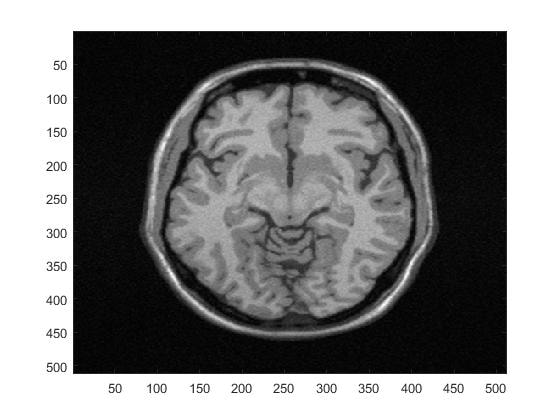
\includegraphics[scale=0.5]{figures/Module_10/Module10_5}\caption{The image after initial interpolation 512x512 pixels}. 
\label{fig: Module10_5}
\end{figure}

\item \textbf{Regularization}
\newline The main functionality is the regularization step. The function makes the square window which contains some pixels. In one iteration of a loop, only the pixels which are inside the window are considered. Next, the window moves and takes another pixels. It is repeated till the end of the image. The main goal is to determine of the weight which will be used at the end.
\newline The first weight is calculated as the difference between the pixels intensities.
\newline 
\centerline {$w_{1}(x, y)= e^{\frac{|N(x)-N(y)|^{2}}{h^{2}}}$, where}
\newline
\newline $N(x)$, $N(y)$ are window and image intensity values,
\newline $h$ is a level, which is equal to the half of the standard deviation of the input image.
\newline The next part of the whole weight is an Euclidean distance weight. It is simply calculated as the Euclidean distance between every pixel in the window and every pixel in the image. It is based on the below equation.
\newline
\centerline{ $w_{2}(x,y)=\frac{\sqrt{(x_{1}-x_{2})^{2}+(y_{1}-y_{2})^{2}}}{h^{2}}$, where }
\newline
\newline $h$ is a level, which is equal to the half of the standard deviation of the input image.
\newline The total weight is calculated as $w_{total}=w_{1}*w_{2}$. The output image is determined as the result of the sum of the multiplication of the weight and the window, divided by the sum of the weight.

\item \textbf{Mean correction}
\newline The mean correction step is a place in the function where the correctness of the equation $X=X+NN*(D(X)-y)$. It was abovementioned, that the downsampled HR has to be equal to the input data.

\item \textbf{Tolerance checking}
At the beginning it was established that only the 2D images will be taken into consideration and the upsampling function will be applied only once, so the step is excluded. There were experiments to upsample the data several times, but the result were not satisfied.

\end{enumerate}


\section{Module 11. Brain 3D}

\indent The implementation of 11th module includes visualization of cortex structure in three-dimensional model and visualization of elected cross-section of model. \\
\indent  As input parameter, module gets ouput of 9th module. This is the mask of segmentated data, which includes cortex structure as value 3. The data about cortex structure is seperated from 3D array.
11 th module is displayed in new window of application, so implementation includes not only functionality requirements but also design of graphical user interface.  \\
\indent To prepare design of user interface used Qt Designer program. \\
\indent Module is selected by user in main window of application. If input data is correct, new window is opened and reconstrucion of three-dimensional model is initialized automatically. \\
\indent First input data – 3D array – is converted to vtkFloatArray, which makes vtkImageData object. Then basing on vtkImageData there is used vtkMarcingCubes class, which makes reconstruction. As a threshold there is used value equal to 1, because of fact that all values not equal to zero are included to cortex structure. \\
\indent After reconstrucion model is displayed in BRAIN 3D window. To enable displaying VTK objects in Qt Application there is set frame in which is inserted the object of VTK library by using QVTKRenderWindowInteractor. It is dedicated vtkWidget to display VTK in QT ibrary.\\
\indent To visualization data there are used following classes:
\begin{itemize}
\item vtkRenderer – which enables rendering process: transforming geometry, light and camera view into an image
\item 
vtkMapper – which maps data to graphics primitives
\item vtkActor – adjusting data to 3D scenery
\item vtkInteractorStyleTrackballCamera – setting possibility of interaction with model
\end{itemize}
\indent BRAIN 3D window enables three options:
\begin{itemize}
\item preview 3D model
\item clip model 
\item clip model and show plane.
\end{itemize}
\indent Automatically after initialization there is loaded firts mode: preview 3D model. 
Mode: clip model, enables to set intersection plane and cut model in place of it. Intersection plane is vtkImagePlaneWidget object. It allows to interactive set the plane by computer mouse. Interaction of plane is activated whenever user presses „clip model” button. When interaction event is detected the model is automatically clipped by vtkCliPolyData class. \\
\indent Mode:  clip model and show plane calls the same function as previous mode, but with input parameter planemode - True ( default – False). It expands functionality of diplaying the cross-section corresponding to the elected plane. It improves readability of intersection plane. It is based on the same objects of VTK library, but using additional methods of it.\\
\indent User has possibility fluently switch modeLs by pressing appropriate buttons. Application has also help window, with short user guide.


\section{Module 12. Oblique imaging}

\indent The literature to this module is as useful as nipples on
men. Everything is about inventing how to realize point 1. of the
list. \\
 \indent Oblique Imaging is a technique to create non-perspective
projections from 3D or multiple 2D images.\\

\indent In order to create oblique image it is essential to: 
\begin{itemize}
\item choose two angles under which the plane will be inclined, 
\item create a matrix of points that this plane consists of, 
\item from existing points pick those, which will be used in the image, 
\item interpolate points that are not existing. 
\end{itemize}
\indent Type of interpolation can vary, but in this project interpolation
based on mean will be used. To interpolate one pixel mean of all pixels
around him with given proximity is taken.

\begin{figure}[H]
\centering{}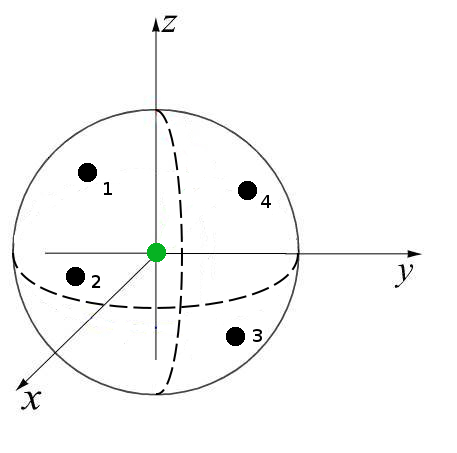
\includegraphics[scale=0.7]{figures/m11_spherexyz}\caption{Visualization of pixels taken to interpolate}
\label{fig:figures/m11_spherexyz } 
\end{figure}



\chapter{Tests}

\section{Module 1. MRI reconstruction}

Classical least squares estimation provides only the minimization of data error, which is an invalid solution. Conventionally, the LSE solution has a huge norm and thus it is a valueless outcome of a~reconstruction procedure. To this end, we introduced basic Tikhonov regularization method that seem to partially overcome the problem. However, we firstly implemented LSE approach for later usage of the results obtained with this procedure in restoration of the images from a~`nearby' well-posed problem (regularization). For Tikhonov regularization, additional quadratic penalty term allows controlling the norm of the solution, which benefits in introduction of smoothness prior to estimated solution. 

Firstly, we checked the data dimension that we load to the programme, as we could receive data starting from 3D to 5D. The implementation works for single slice structural and diffusion data (from many gradients) as well as for a whole set of brain slices. First two dimensions, provides information about data resolution i.e. $128\times 256$, which means that the images where subsampled with factor $r=2$. In case of structural data, the third dimension would be the number of slices (then, the forth is number of coils images) or simply number of coils images. For diffusion data, in 5D case the third dimension stands for number of slices, the forth - number of diffusion gradients and the fifth - number of coils images. The third dimension can be equal to one, so we get 4D data i.e. diffusion data for one slice. We also tested whether input dataset contains matrices with sensitivity maps profiles of a proper size, corresponding to maximal dimension of an image i.e. $256\times 256\times 8$, for case of images acquired with $8$ coils. Furthermore, the input files should also contain subsampling factor $r$ and number of coils $L$, if not, they can be calculated having the dataset's dimensional information.
 
Secondly, we performed 2D inverse Fourier Transform (2D IFT) on each of the dataset image, to transform them from \textbf{k}-space to \textbf{x}-space. This stage of an algorithm is presented in Fig. \ref{rys:subsampled}.  

\begin{figure}[h!]
\centering
  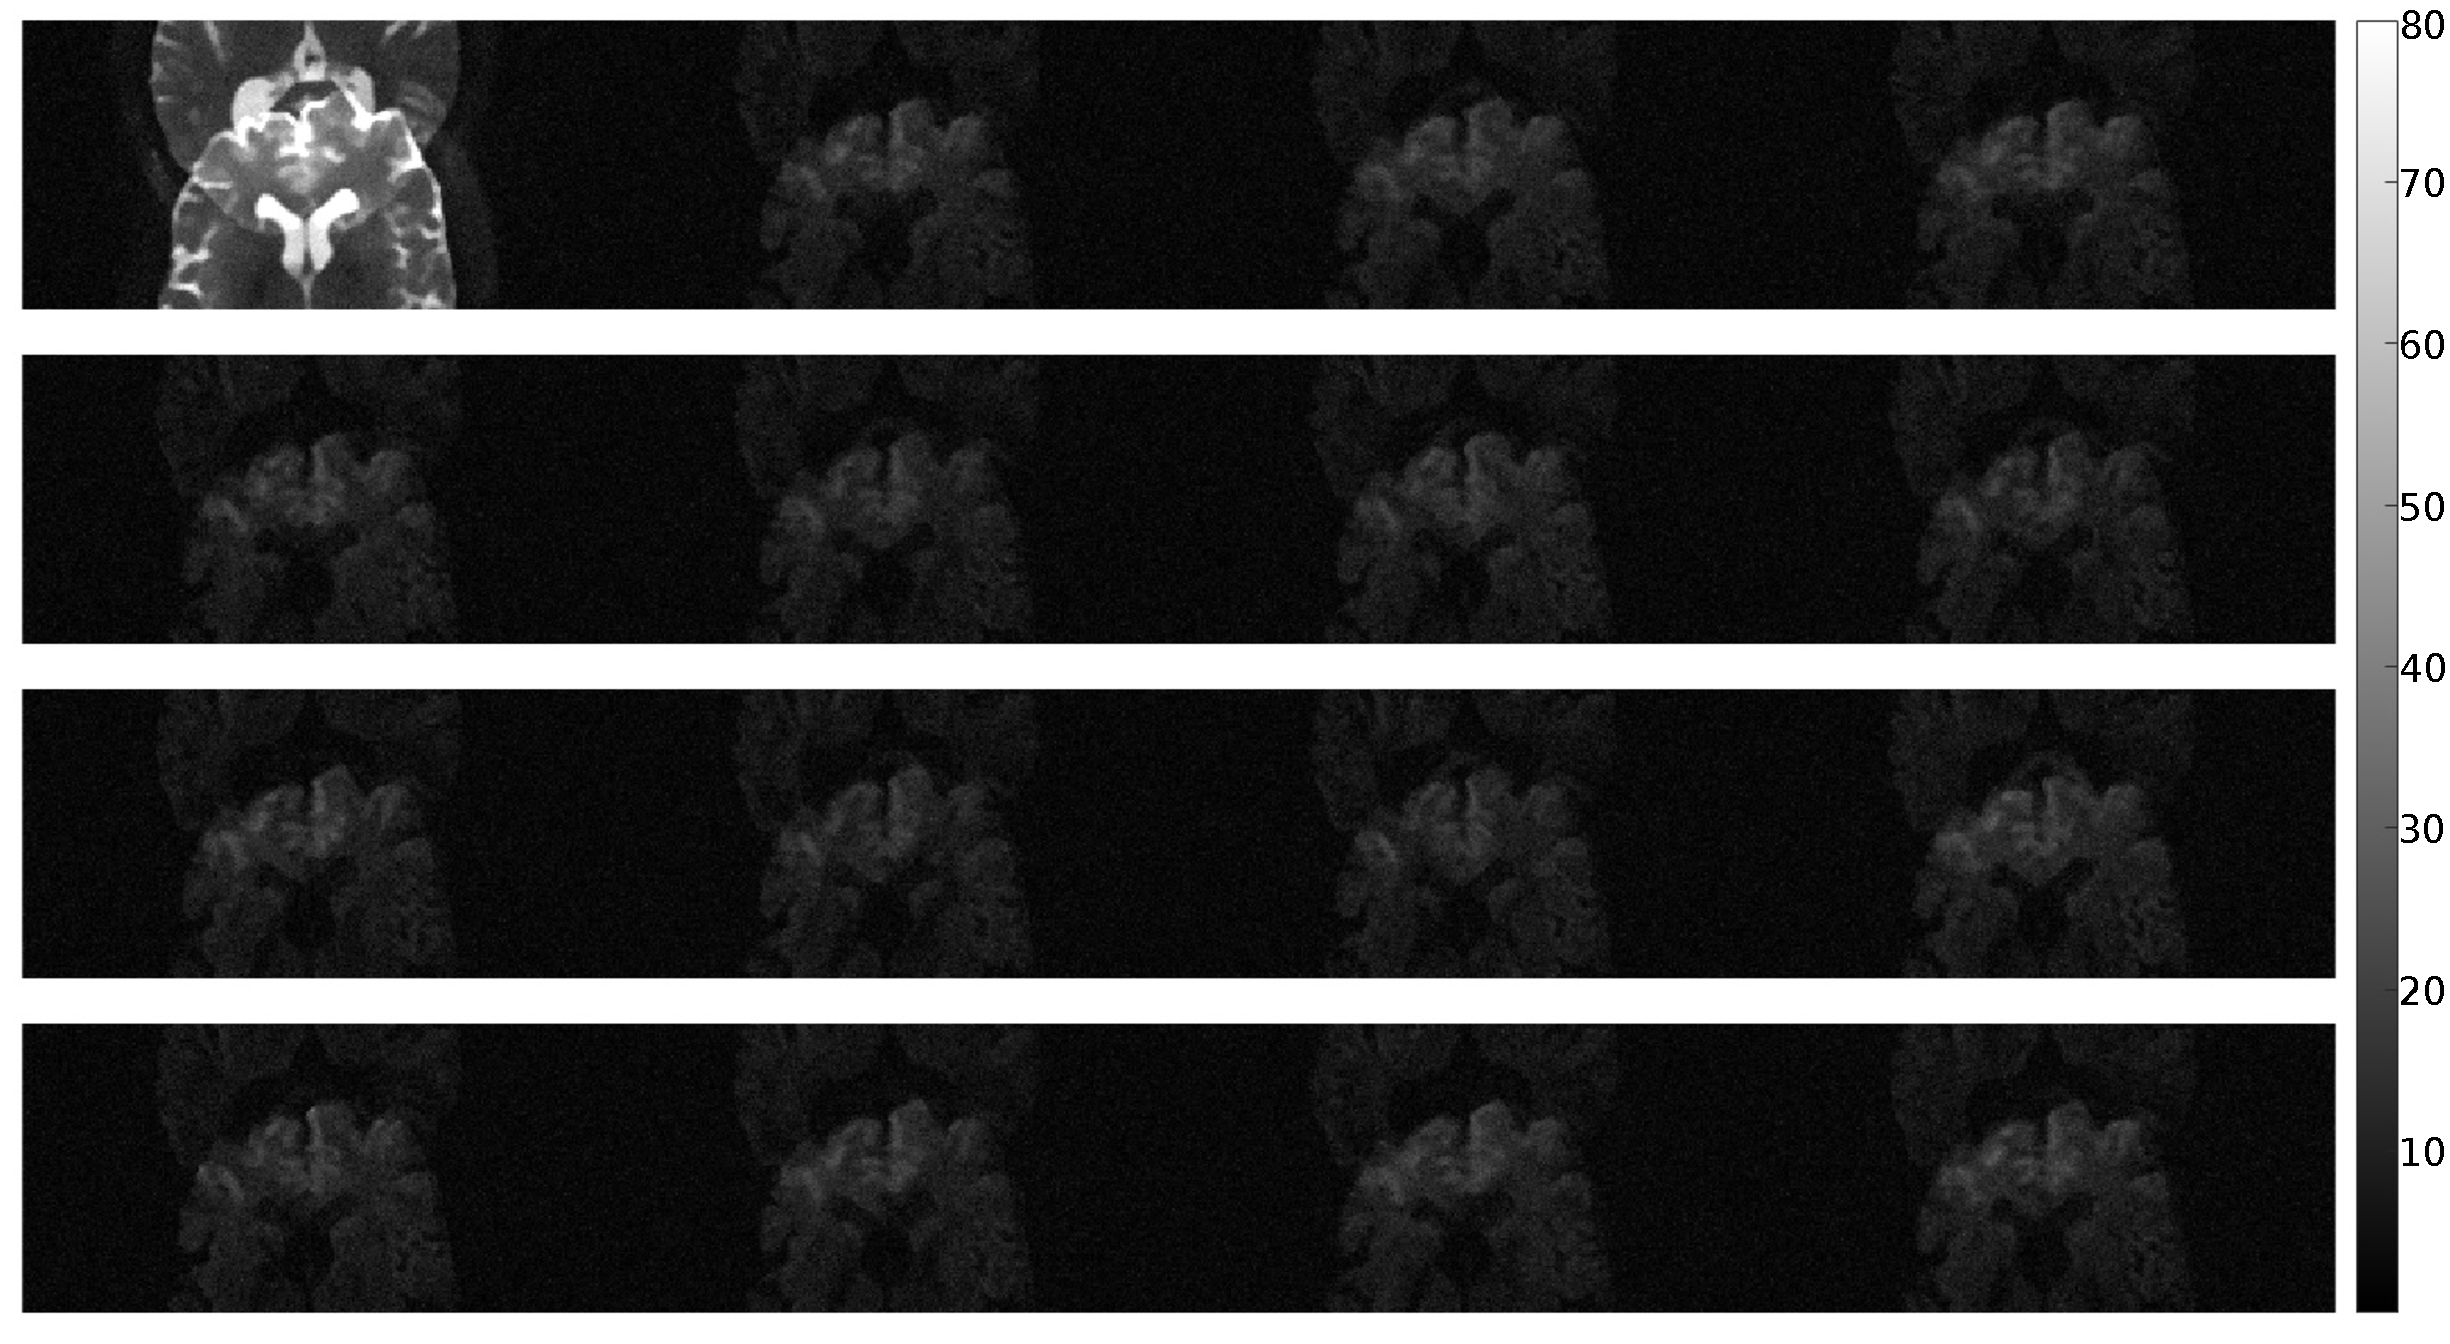
\includegraphics[scale=0.36]{figures/Module_01/NON_RECON.pdf}
  \caption{Subsampled diffusion dataset in \textbf{x}-space domain (data for one particular slice, acquired for 15 diffusion weightening gradients).}
  \label{rys:subsampled}
\end{figure}

\begin{figure}[h!]
\centering
  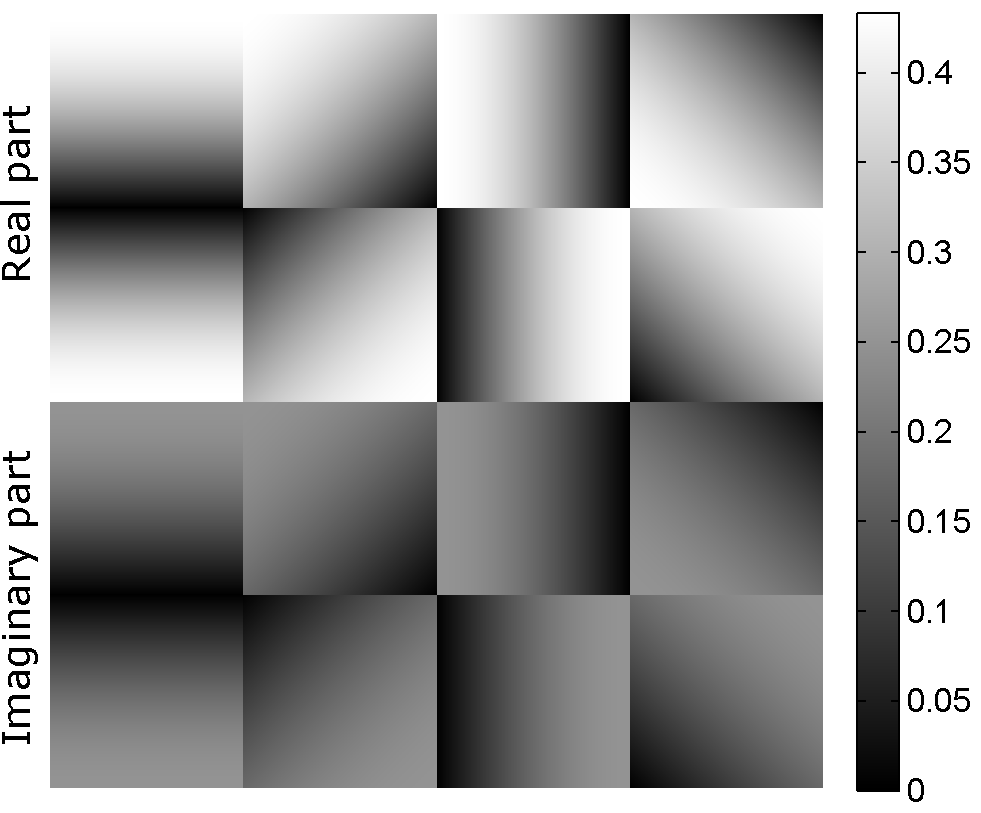
\includegraphics[scale=0.46]{figures/Module_01/MAPS.pdf}
  \caption{The real and imaginary parts of sensitivity maps used to reconstruct data ($L = 8$).}
  \label{rys:maps}
\end{figure}

\begin{figure}[h!]
\centering
  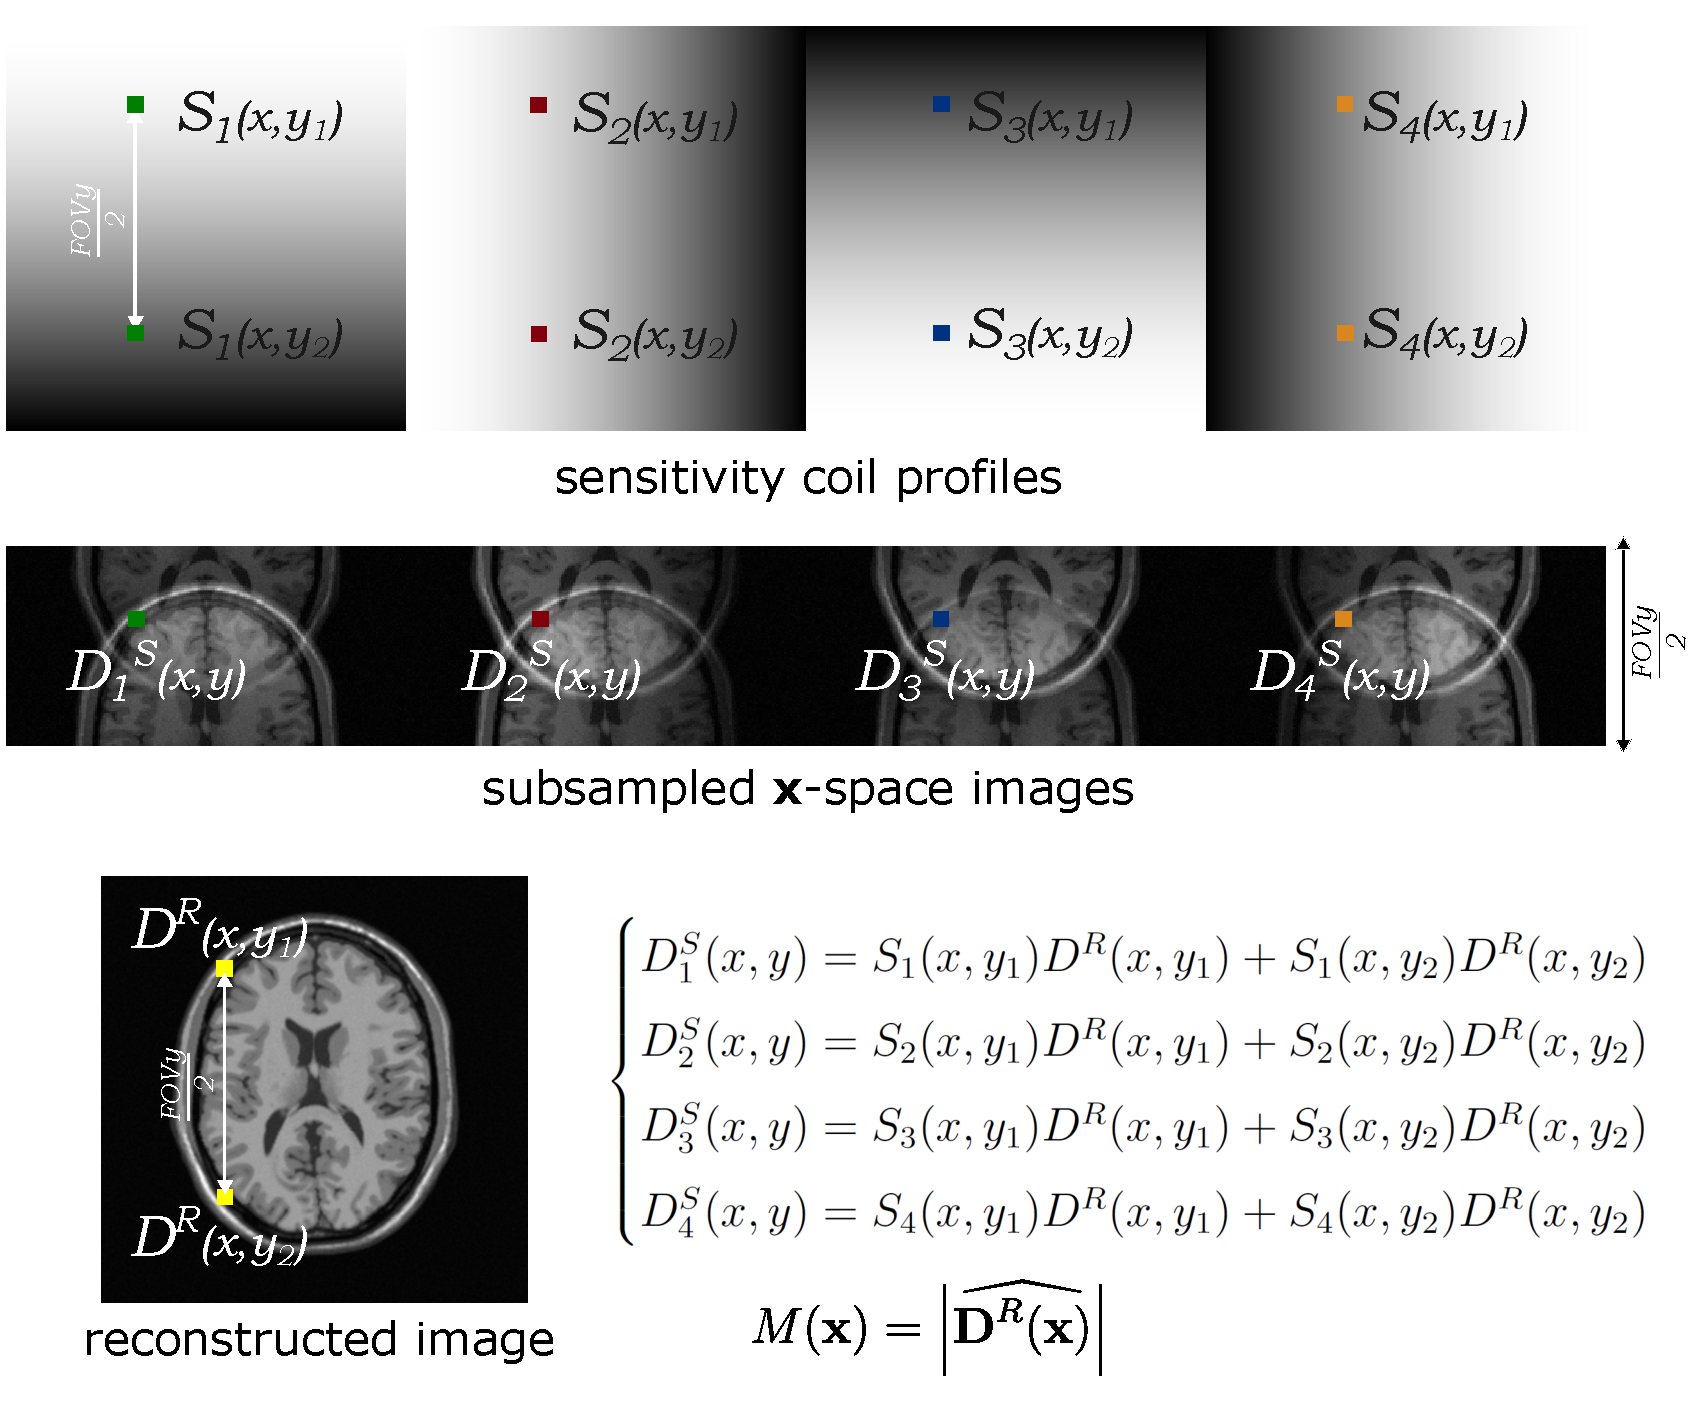
\includegraphics[scale=0.36]{figures/Module_01/SENSE.pdf}
  \caption{SENSE algorithm graphical explanation of Cartesian sampling using four receiver
coils ($L = 4$) and the subsampling rate $r = 2$. Two yellow pixels of the reconstructed image are
unfolded using coil sensitivity profiles and the corresponding folded pixels (points marked with
green, red, blue and orange).}
  \label{rys:sense}
\end{figure}

Thirdly, we used absolute value operator right before performing the SENSE reconstruction main step. As we are provided with sensitivity maps profiles (Fig. \ref{rys:maps}), we can easily reconstruct the subsampled data as it is shown in Fig. \ref{rys:sense}.
The key idea is to evaluate the algorithm pixel by pixel. According to equation \ref{Eq:wzor4}, the construction of defined $\textbf{D}^{S}$ vector is simple. Basically, the $\textbf{D}^{S}$ is a column vector of $L\times1$ size, containing pixels withdrawn from each $L$ coil image at specified spatial location. The matrix $\textbf{S}$ we construct in a~subsequent way: the $l-th$ row of $\textbf{D}^{S}$ contains values of the sensitivity maps profiles, corresponding to data position in a subsampled image and moved by a subsampled FOV value (i.e. for $r=4$, $FOV_{y} = 256/4 = 64$) $r-1$ times. As a result, depending on the number of coils and subsampling rate value, we obtained a matrix of $L\times r$ size. In LSE sense, the result of computation of  for defined $\textbf{D}^{S}$ and~$\textbf{S}$ is column vector $\textbf{D}^{R}$ ($r\times 1$ size). 

However, the LSE approach is not an optimal solution, so we implemented the regularization approach which uses the \textit{a priori} information of searched solution obtained with LSE algorithm. The images obtained after first reconstruction are median filtered with window size$3$x$3$. We introduced this additional information to the solution of derived objective function according to Eq. \ref{Eq:wzor7}. In this case, $\textbf{D}^{S}$ and~$\textbf{S}$ are constructed in the same manner as for LSE case, however we regularized the solution with $\lambda$ parameter. The choice of appropriate value of regularization parameter allows controlling the balance between both components (bias-variance tradeoff). For this scenario, we empirically picked $\lambda$ parameter as a constant value. As the reconstruction is performed pointwisely, we introduced extra information about expected result as a vector $\textbf{D}$ of $r$x$1$ size, containing pixels from reconstructed median filtered LSE images corresponding spatially to those to be reestimated with Tikhonov approach. The result is similar, i.e., we derived values of $r$ reconstructed points, which differ from those obtained with basic LSE approach. Fig. \ref{rys:recon} presents exemplary result of Tikhonov reconstruction algorithm implemented in the software. 

\begin{figure}[h!]
\centering
  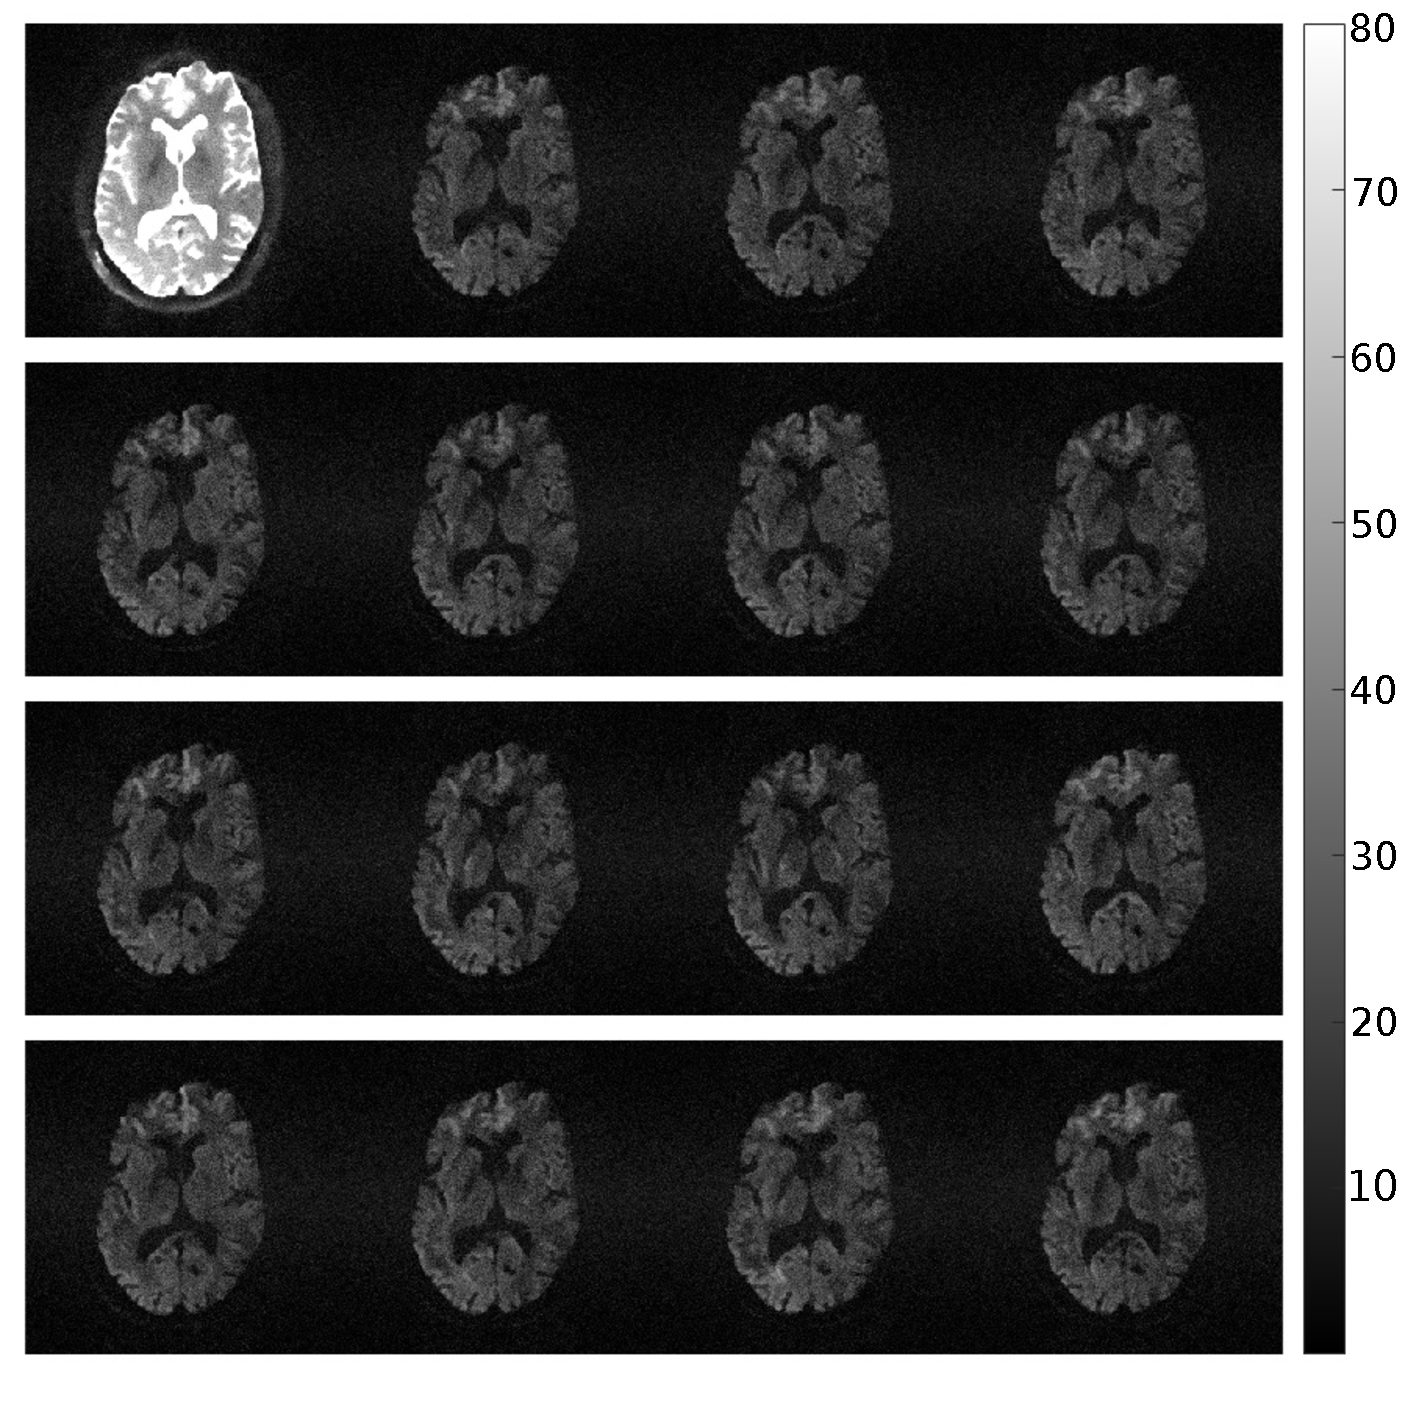
\includegraphics[scale=0.36]{figures/Module_01/RECON.pdf}
  \caption{Reconstructed diffusion dataset in \textbf{x}-space domain (data for one particular slice, acquired for 15 diffusion weightening gradients).}
  \label{rys:recon}
\end{figure}



\section{Module 2. Intensity inhomogeneity correction}

The Intensity inhomogeneity of the same tissue varies with the location
of the tissue within the image. In other words it refers to the slow,
nonanatomic intensity variations of the same tissue over the image
domain. It can be due to imaging instrumentation (such as radio-frequency
nonuniformity, static field inhomogeneity, etc.) or the patient movement.
This artifact is particularly severe in MR images captured by surface
coils. Although intensity inhomogeneity is usually hardly noticeable
to a human observer, many medical image analysis methods, such as
segmentation and registration, are highly sensitive to the spurious
variations of image intensities.

The aim of this module is estimation of intensity inhomogeneity field in MR image using surface fitting method. The method fits a parametric surface to a set of image features that contain information on intensity inhomogeneity. The resulting surface, which is usually polynomial or spline based, represents the multiplicative inhomogeneity field that is used to correct the input image.

The steps of this approach are: 
\begin{enumerate}
\item {Extract a background image from the corrupted MRI image, for example, by smoothing the image with a Gaussian filter of a large bandwidth (about 2/3 the size of the MRI image) to filter out all the image details that correspond to highfrequency components.}
\item {Select few data points from the background image and save their coordinates and graylevel values into a matrix $D = (xi , yi , gi), i = 1, 2, ...n$. It is recommended not to select points from the regions where there is no MRI signal since this regions has no bias field signal.}
\item {Select a parametric equation for the fitted surface . It is better to fit simple surfaces such as low order polynomial surfaces since they are very smooth and their parameters are very easy to estimate.}
\item {Estimate the parameters of the surface that best fits the data in matrix D by the method of nonlinear least-squares.}
\item {Use the fitted equation to generate an image of the bias field signal.}
\item {Divide the corrupted MRI image by the estimated bias field image in step 5.} 
\end{enumerate}
Even though different surfaces can reasonably fit the data very well and it is not possible to tell which surface is most likely represents the actual bias field signal, however, in practice the bias signal estimated by fitting a smooth 2-dimensional polynomial surface to a background image can be used effectively to restore the corrupted MRI image.

Fitting of the surface can be done by means of the Levenberg-Marquardt algorithm for nonlinear least squares fitting of a function $f(x, y; a_{1}, ..., a_{m})$ of known form to $n$ data points ${(x_{1}, y_{1}, g_{1}), ...,(xn, yn, gn)}$. For example, a polynomial surface of degree three can be fitted which has the following equation: $f(x, y; a) = a_{1}x^{3} + a_{2}y^{3} + a_{3}$, where $a = {a_{1}, a_{2}, a_{3}}$ is the parameter vector that define the surface. If we substitute the data points in the nonlinear function we get an overdetermined set of equations, i.e.,
\begin{equation}
\begin{Bmatrix}
g_{1} = f(x_{1}, y_{1}; a_{1}, a_{2}, ..., a_{m})\\ 
\cdot                                            \\
\cdot                                            \\ 
g_{n} = f(x_{n}, y_{n}; a_{1}, a_{2}, ..., a_{m})\\ 
\end{Bmatrix}
\end{equation}
These equations can be solved to obtain the unknown parameter vector $(a_{1}, a_{2}, ..., a_{m})$ by minimizing the sum of the squares of the differences between the data and the fitted function
\begin{equation}
\begin{aligned}
Q(\textbf{a})=\dfrac{1}{2} \sum_{i=1}^{n}(g_{i} - f(x_{i},y_{i}; a_{1},a_{2}, ...,a_{m}))^{2}
\label{fig: eq2_1}
\end{aligned}
\end{equation}
Let $r_{i}(\textbf{a}) = (g_{i} - f( x_{i}, y_{i}; a_{1}, a_{2}, ..., a_{m})$, which is the residual vector of point $i$, then equation \ref{fig: eq2_1} can be written as:
\begin{equation}
\begin{aligned}
Q(\textbf{a})=\dfrac{1}{2} \sum_{i=1}^{n}(r_{1}(\textbf{a}))^{2}
\label{fig: eq2_2}
\end{aligned}
\end{equation}
According to the Levenberg-Marquardt algorithm, eq.\ref{fig: eq2_2} can be solved iteratively to find the values of the parameters vector ($\textbf{a}$) starting from an initial estimate of the parameter vector $(\textbf{a}_{0})$ using:
\begin{equation}
\begin{aligned}
\textbf{a}_{i+1} = \textbf{a}_{i} - (H + \lambda diag[H])^{-1} \bigtriangledown Q(\textbf{a}_{i})
\label{fig: eq2_3}
\end{aligned}
\end{equation}
where $H$ and $\bigtriangledown$Q($\textbf{a}_{1}$) are Hessian matrix and the gradient of Eq. \ref{fig: eq2_2} both evaluated at $a_{i}$, $diag[H]$ is the diagonal elements of the Hessian matrix. At each iteration, the algorithm tests the value of the residual error  and adjusts $\lambda$ accordingly. \cite{2a1}

\section{Module 3. Non-stationary noise estimation}
In order to test effectiveness of implemented algorithm the results of it were compared to results of algorithm prepared to perforem calculatioans contained in \cite{aja2015spatially}. The algorithm for the article was implemented in Matlab.
\begin{figure}[H]
	\centering{}
		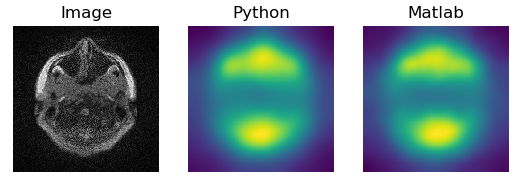
\includegraphics[scale=0.7]{figures/module03/10_comp}
	\caption{Image (left), noise map form Python algorithm(middle), noise map form Matlab algorithm(right).} 
\end{figure}
\begin{figure}[H]
	\centering{}
		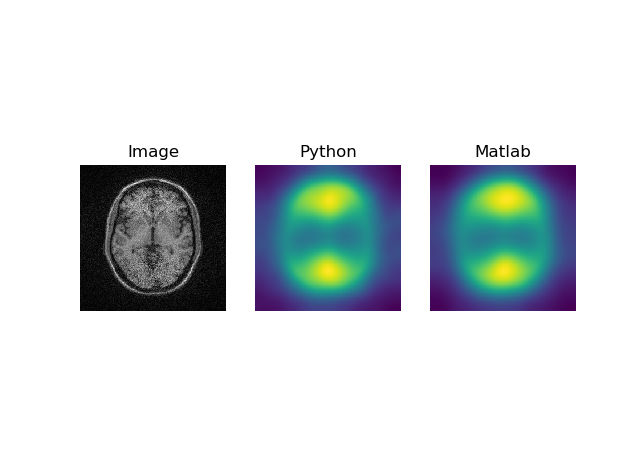
\includegraphics[scale=0.7]{figures/module03/70_comp}
	\caption{Image (left), noise map form Python algorithm(middle), noise map form Matlab algorithm(right).} 
\end{figure}
\begin{figure}[H]
	\centering{}
		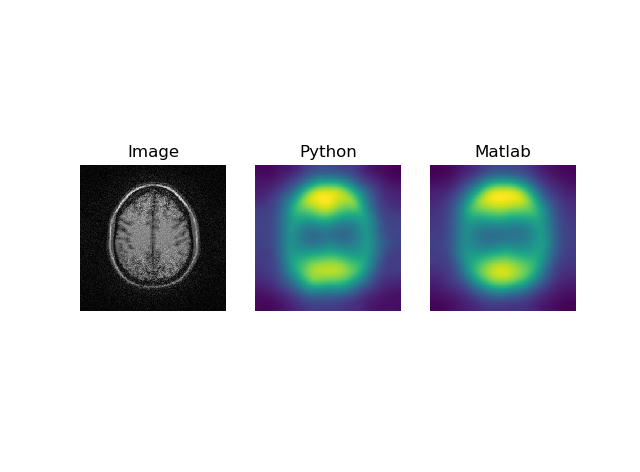
\includegraphics[scale=0.7]{figures/module03/110_comp}
	\caption{Image (left), noise map form Python algorithm(middle), noise map form Matlab algorithm(right).} 
\end{figure}
\begin{figure}[H]
	\centering{}
		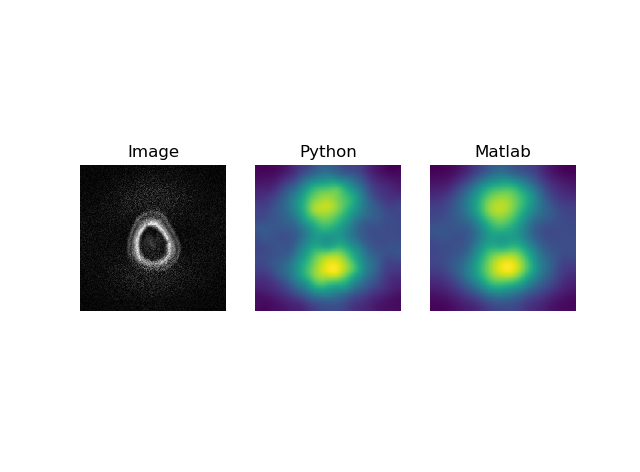
\includegraphics[scale=0.7]{figures/module03/160_comp}
	\caption{Image (left), noise map form Python algorithm(middle), noise map form Matlab algorithm(right).} 
\end{figure}
Results from Python algorithm are not perfect equivalent of the results from Matlab algorithm however ther are very similar and seem to be suitable for 
further processing of the image.

\section{Module 4. Non-stationary noise filtering 1}

The aim of this module is to remove Rician noise from MR images. If
both real and imaginary parts of signal are corrupted with zero-mean
uncorrelated Gaussian noise with equal variance, the envelope of magnitude
signal will follow a Rician distribution. Many processes allow to
remove noise, here the method is used to denoise MR images is the
linear minimum square error estimator (LMMSE). The main purpose of
LMMSE is to find a closed-form estimator for a signal that follows
a Rician distributions. It is more efficient than optimization-based
solutions. The estimator uses information of the sample distribution
of local statistics of the image such as the local mean, the local
variance and the local mean square value. In this method, the true
value for each noisy pixel is estimated by a set of pixels selected
from a local neighborhood.

The LMMSE estimator for a 2-D signal with Rician distribution is defined:

\begin{equation}
\begin{aligned}\widehat{A_{ij}^{2}}=E\{A_{ij}^{2}\}+C_{A_{ij}^{2}M_{ij}^{2}}C_{M_{ij}^{2}M_{ij}^{2}}^{-1}(M_{ij}^{2}-E\{M_{ij}^{2}\})\end{aligned}
\label{m4eq1}
\end{equation}
where $A_{ij}$ is the unknown intensity value in pixel $ij$, $M_{i}j$
the observation vector, $C_{A_{ij}^{2}M_{ij}^{2}}$ the cross-covarience
vector and $C_{M_{ij}^{2}M_{ij}^{2}}$ the covarience matrix. If the
estimator is simplified to be pointwise, vectors and matrics become
scalar values. Then the assuming local ergodicity with a square nighbourhood
around the pixel $ij$, the finally equation for LMMSE is defined:
\begin{equation}
\begin{aligned}\widehat{A_{ij}^{2}}=\langle M_{i}j^{2}\rangle-2\sigma_{n}^{2}+K_{ij}(M_{ij}^{2}-\langle M_{ij}^{2}\rangle)\end{aligned}
\label{m4eq2}
\end{equation}
with $K_{ij}$ 
\begin{equation}
\begin{aligned}K_{ij}^{2}=1-\frac{4\sigma_{n}^{2}(\langle M_{i}j^{2}\rangle-2\sigma_{n}^{2})}{\langle M_{i}j^{4}\rangle-{\langle M_{i}j^{2}\rangle}^{2}}\end{aligned}
\label{m4eq3}
\end{equation}

The LMMSE estimator is related to the quality of the estimate of the
noise variance $\sigma_{n}^{2}$. For the noise estimation the mode
of the sample mean is used:

\begin{equation}
\begin{aligned}\widehat{\sigma_{n}}=\sqrt{\frac{2}{\pi}}mode(\widehat{\mu_{1}}_{ij})\end{aligned}
\label{m4eq4}
\end{equation}
where $\widehat{\mu_{1}}_{ij}$ 
\begin{equation}
\begin{aligned}\widehat{\mu_{1}}_{ij}=\frac{1}{|\eta_{ij}}\sum_{p\colon\eta_{ij}}I_{p}\end{aligned}
\label{m4eq5}
\end{equation}

The use of the LMMSE method should makes the filtering process computationally
far more efficient and easier to implement. Also the use of local
statistics should decrease estimator dependent of parameters such
as the size of window.

\textbf{\emph{Module input}}: Reconstructed, normalized and corrected
data.

\textbf{\emph{Module output}}: Image without Rician noise.

\section{Module 5. Non-stationary noise filtering 2}

Magnetic Resonance images are endangered of being corrupted by noise
and artifacts. Since they are used as a basis for medical diagnosis
their quality has to be at highest possible level. Noise can be dealt
with by changing the parameters of images acquisition, however it
increases the scanning time, which is undesirable in medical imaging.
To overcome this obstacle, post-processing methods like filtering
are employed for denoising. In domain of MRI denoising many filters
may be used, though here emphasis is put on Unbiased Non-Local Means
(UNLM) filter, which is an extension of NLM filter. In order to understand
Unbiased version of this algorithm, the basic one has to be presented.

Having image \textit{Y}, the NLM algorithm calculates the new value
of point \textit{p} accordingly to the equation:

\begin{equation}
\begin{aligned}NLM(Y(p))=\sum_{\forall q\in Y}^ {}w(p,q)Y(q)\\
0\le w(p,q)\le1,\sum_{\forall q\in Y}^ {}w(p,q)=1
\end{aligned}
\label{m5e1}
\end{equation}

It can be seen that value of \textit{p} is calculated as weighted
average of pixels in the image (\textit{q}), having fulfilled restrictions
from \ref{m5e1}. To determine before mentioned average the similarity
between square neighbourhoods widows centered around pixels \textit{p}
and \textit{q} are calculated. The size of the window can determined
by the user, defined by parameter $R_{sim}$. Equation \ref{m5e2}
shows how to determine this similarity.

\begin{equation}
w(p,q)=\frac{1}{Z(p)}e^{\dfrac{d(p,q)}{h^{2}}}\label{m5e2}
\end{equation}

\textit{Z(p)} is the normalizing constant which also uses exponential
decay parameter \textit{h} and the weighted Euclidean distance measure
for pixels in each neighbourhood, called \textit{d}.

\begin{equation}
Z(p)=\sum_{\forall q}^ {}e^{\dfrac{d(p,q)}{h^{2}}}\label{m5e5}
\end{equation}

\begin{equation}
d(p,q)=G_{p}||Y(N_{p})-Y(N_{q})||_{R_{sim}}^{2}\label{m5e6}
\end{equation}

In above equation $G_{p}$ stands for a Gaussian weighting function
that has a 0 mean and standard deviation usually equal to 1.


Once NLM filter is fully explained, unbiased extension of it can be
examined. It builds on the properties of MRI signal. According to
\cite{5a1} the magnitude signal of MRI follows a Rician distribution.
Furthermore, for low intensity regions the Rician distribution approaches
to a Rayleigh one, whilst for high intensity it shifts towards Gaussian.
It was investigated that this bias can be handled by filtering the
squared MRI image, since it is not longer signal-dependent \cite{5a1}.
As a consequence the bias, which equals 2$\sigma^{2}$ \cite{5a3}
can be deleted with ease. The blueprint for UNLM can be summarized
in:
\begin{itemize}
\item noise estimation - which can be done by calculating standard deviation
of background in the image. To distinguish
background and the body on the MRI scan the Otsu thresholding method
\cite{5a4} can be successfully used. In this version noise maps are used, to achieve
non-stationary noise filtration, 
\item calculating NLM values for each point of image as in \ref{m5e1}, 
\item assessing the unbiased value of each point accordingly to the equation
\ref{m5e3}.
\end{itemize}
\begin{equation}
UNLM(Y)=\sqrt{NLM(Y)^{2}-2\sigma^{2}}\label{m5e3}
\end{equation}

In above equation $\sigma$ refers to value of non-stationary noise in the signal, more precisely
it is a value for each pixel from the original image, stored in a form of noise map.

% dwi, if it has to be joint implementation 
UNML implementation for diffusion weighted data becomes a bit less
trivial task, due to the new dimension of data associated with different gradients for each slice.
Based on assumption that gradients in similar directions
present related behaviours, UNLM for DWI can be formulated as:

\begin{equation}
Y_{i}(p)=\sqrt{\sum_{j\in\Theta_{i}^{N}}^ {}\sum_{q\in N_{p}}^ {}w_{i}^{j}(p,q)M_{j}^{2}(q)-2\sigma^{2}}
\end{equation}

Where weights are calculated as for structural data and \textit{M}
is a vector containing gray values.

\begin{equation}
d_{i}^{j}(p,q)=(M_{i}(N_{p})-M_{j}(N_{q}))^{T}G_{p}(M_{i}(N_{p})-M_{j}(N_{q}))\label{m5e7}
\end{equation}

However it was reported in \cite{5a2} that denoising diffusion weighted data using
UNLM method gives no significant results, so gradients related data can be ignored, or 
filtered as structural data.

It is worth mentioning that UNLM filter's performance is highly dependent
on parameter values. The optimal values of them were examined in \cite{5a1}
and same values are adapted in presented implementation. Properly-tuned
filter can significantly increase SNR of the scans while preserving
body structures.

\textbf{\emph{Module input}}: Previously reconstructed, normalized
and corrected data, noise maps.

\textbf{\emph{Module output}}: Image with deleted Rician noise by
unbiased non-local means filter. \\

\section{Module 6. Diffusion tensor imaging}

\textbf{Preprocessing and Module I/O}

In order to improve diffusion tensor estimation it is imperative to
remove artifacts. In addition to standard MRI pre-processing, one
needs to correct for artifacts arising the use of diffusion-gradient
pulse sequences and longer acquisition time. While hardware manufacturers
try to proactively diminish some of these effects, software processing
is still mandatory. 
\hfill\\

\textbf{Module Input}:
\begin{itemize}
	\item 
	3D structural data array of shape X x Y x Z, where XY - pixel image intensities, Z - chosen slice, which is the T1- or T2-weighted image corresponding the the given DWI acquisition
	
	\item 
	4D diffusion data array of shape X x Y x Z x M, where XY - pixel image intensities, Z - chosen slice, M - applied diffusion gradient direction
	
	\item 
	b\_value, a scalar value corresponding to applied diffusion gradient sequence magnitude
	
	\item 
	2D gradients matrix of shape M x 3, where each row corresponds to a normalized $(x,y,z)$ components of diffusion gradient sequence vectors
		
	\item 
	optionally - 3D binary mask of shape X x Y x Z, corresponding to the brain area detected by Module 8 (Skull Stripping); if not supplied, DTI is computed on each input data voxel

\end{itemize}
\hfill

\textbf{Module Output}:
\begin{itemize}
	\item
	list of size Z, corresponding to each slice; every list element is a dictionary of biomarker images: MD, RA, FA, VR of shape X x Y, and biomarker FA\_rgb of shape X x Y x 3
\end{itemize}

\subsection{Initialization}

In order to abstract DTI implementation from end-user, all classes and methods other than the main function \texttt{run\_module} are private to module source code script. It is important to note that prior to running the module one has to provide the module with input data object, as well as SOLVER and FIX\_METHOD parameters. SOLVER passed as an argument decides whether to use WLS or NLS estimation, whole FIX\_METHOD decides how to "fix" negative eigenvalues. 

As mentioned in the detailed description chapter, 'ABS' takes absolute value of each eigenvalue, while 'CHOLESKY' ensures that the estimated tensor is positive definite. Eigenvalues of positive definite matrices are always non-negative. 'ABS' is a post-estimation fix, meaning that it does not modify the default estimation algorithm (i.e. it is applied after WLS or NLS computation), while 'CHOLESKY' directly modifies the expressions for WLS and NLS cost function gradients and Hessian matrices.

After passing all required arguments to the \texttt{run\_module} function, they are reshaped internally in order to be compatible with module. Concretely, \texttt{DTISolver} class instance, computing the DTI proper, assumes that input data argument is a concatenated 3D array of both structural and diffusion images, which are stored separately in the original data structure. Moreover, b\_value and gradient fields are reshaped to be lists correpsonding to each slice of the new data array (that is: b\_value is repeated in length while both have zeros appended that correspond to structural images). Finally, all of the above is done separately for each slice and DTI module performs it's computation slice-by-slice due to memory constraints.

\subsection{WLS estimation}

WLS with the ABS fix method is a fast yet simple method of module pipeline computation based on diffusion tensor estimation. As such these parameters were set as default for DTI.

Diffusion tensor estimate was computed by implementing the equation:
\begin{equation}
\begin{aligned}
\boldsymbol{\gamma}=\left(\boldsymbol{W}^T\boldsymbol{\omega}^T\boldsymbol{\omega}\boldsymbol{W}\right)^{-1}\boldsymbol{W}^T\boldsymbol{\omega}^T\boldsymbol{\omega y}
\end{aligned}
\label{Eq:m6_impl_eq_1}
\end{equation}

using NumPy matrix broadcasting operations, effectively abstracting away array reshaping. Weights vector $\boldsymbol{\omega}$ is calculated using a separate function in order to avoid changing every piece of code refering to WLS weights in case they change. The following implementation assumes the simplest of models presented in the Detail Description chapter, that is weights being equal to the measured signal.

\subsection{NLS estimation}

In case of NLS estimation, in addition to implementing gradient and Hessian matrix computation methods:

\begin{equation}
\begin{aligned}
\nabla{f_{NLS}}&=-\boldsymbol{W}^T\boldsymbol{\hat{S}}\boldsymbol{r} \\
\nabla^2{f_{NLS}}&=\boldsymbol{W}^T\left(\boldsymbol{\hat{S}^T\hat{S}-\boldsymbol{R\hat{S}}}\right)\boldsymbol{W}
\end{aligned}
\label{Eq:m6_impl_2}
\end{equation}

It is important to devise an iterative scheme because gradient result depends on NLS diffusion tensor estimate. For that reason an algorithm based on \cite{m6_koay2006a} has been implemented. The method itself is called a Modified Newton's Algorithm and can be summarised as in Fig.\ref{fig:m6_pic_1}.

\begin{figure}[H]
	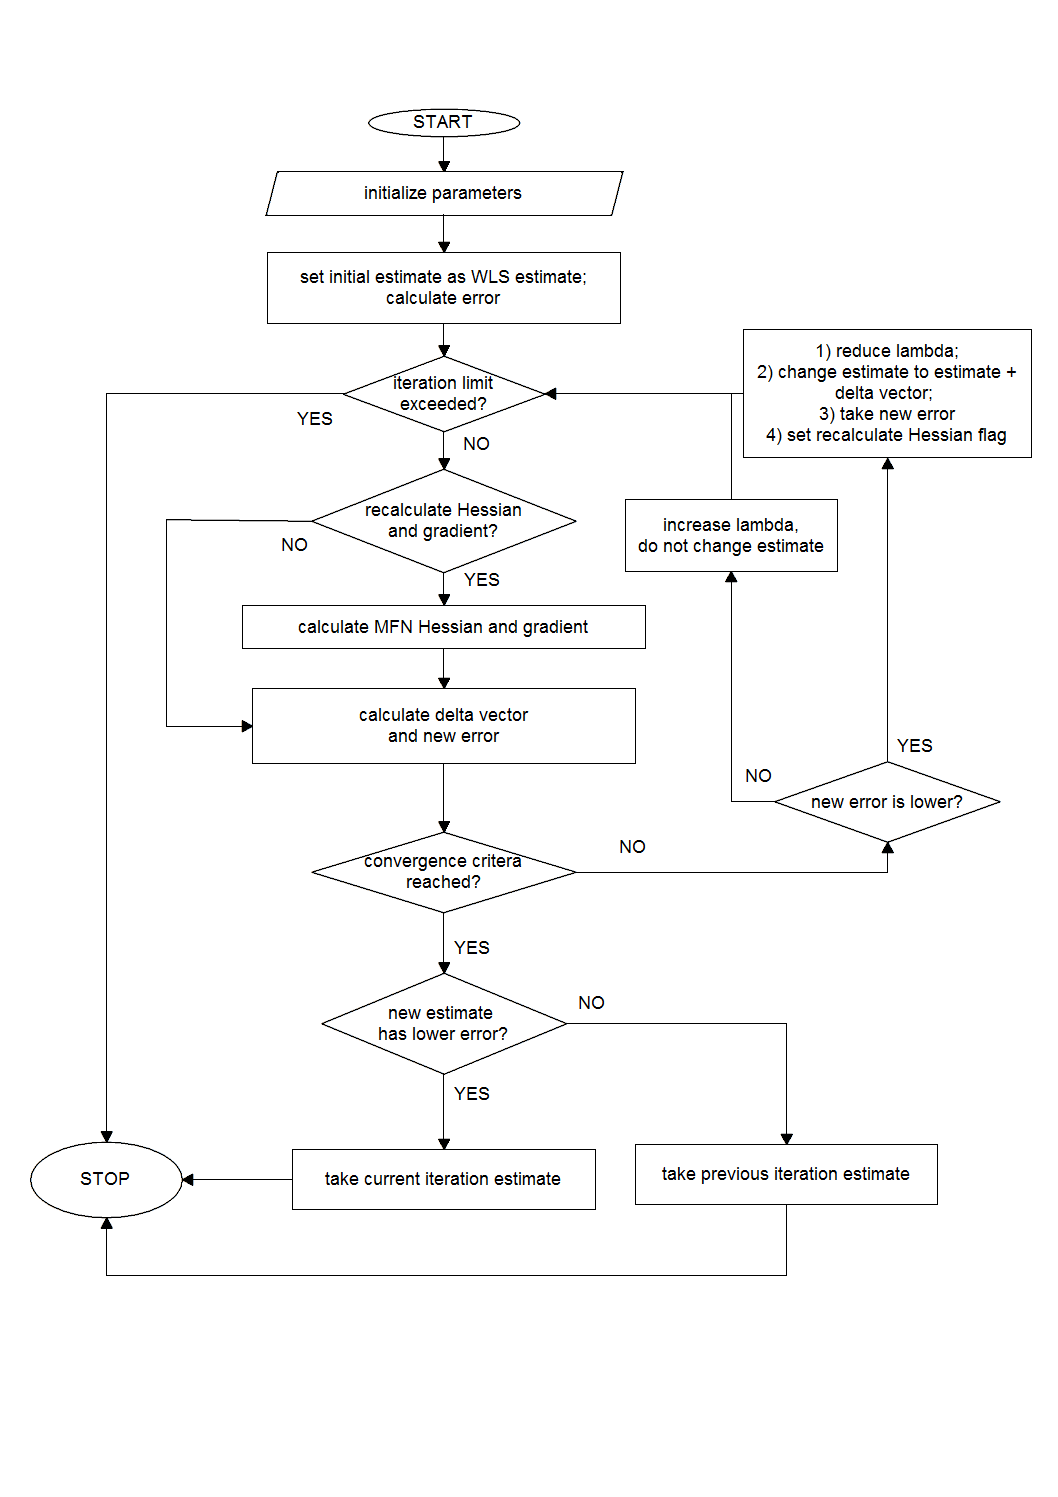
\includegraphics[width=8cm]{figures/Module_06/mfn_simple}
	\centering
	\caption{Modified Newton's method for iterative computation of NLS estimate \vbox{(based on \cite{m6_koay2006a})}}.
	\label{fig:m6_pic_1}
\end{figure}

The following parameters (collectively known in code as MFN parameters) were set:
\begin{itemize}
	\item 
	MFN\_MAX\_ITER = 3 - iteration limit
	
	\item
	MFN\_ERROR\_EPSILON = 1e-5 - first convergence criterion (error change is small)
	
	\item
	MFN\_GRADIENT\_EPSILON = 1e-5 - second convergence criterion (vanishing gradient)
	
	\item
	MFN\_LAMBDA\_MATRIX\_FUN = 'identity'- regularization matrix added to Hessian matrix
	
	\item 
	MFN\_LAMBDA\_PARAM\_INIT = 1e-4 - initial regularization matrix multiplier
\end{itemize}

Delta estimate is calculated using the following formula:
\begin{equation}
\boldsymbol{\delta}=-\left(\nabla^2{f_{NLS}+\lambda I}\right)^{-1}\nabla{f_{NLS}}
\label{Eq:m6_impl_3}
\end{equation}

with $\lambda$ parameter increasing and decreasing by a factor of 10, depending on whether newly calculated estimate yields lower error (decreasing for lower error, increasing otherwise).

Convergence is established using the following formulas:
\begin{equation}
\begin{aligned}
\left|f_{NLS_{new}} - f_{NLS_{new}}\right| &< \texttt{MFN\_ERROR\_EPSILON} \\
\delta^T\nabla{f_{NLS}} &< \texttt{MFN\_GRADIENT\_EPSILON}
\end{aligned}
\end{equation}

\subsection{Biomarkers computation}

As mentioned previously, the estimate obtained from NLS or WLS methods can be reshaped to a 3x3 matrix:
\begin{equation}
\boldsymbol{D}=
\begin{bmatrix}
D_{xx} & D_{xy} & D_{xz} \\
D_{yx} & D_{yy} & D_{yz} \\
D_{zx} & D_{zy} & D_{zz} 
\end{bmatrix}
\label{Eq:m6_impl_4}
\end{equation}
assuming our estimate is equivalent to:
\begin{equation}
\boldsymbol{\gamma}={\lbrack ln{S_0}, D_{xx}, D_{yy}, D_{zz}, D_{xy}, D_{yx}, D_{xz}\rbrack}^T
\label{Eq:m6_impl_5}
\end{equation}

Tensor estimation results for a sample 126x126x55 slice are presented on Fig.\ref{fig:m6_pic_2}.

\begin{figure}[H]
	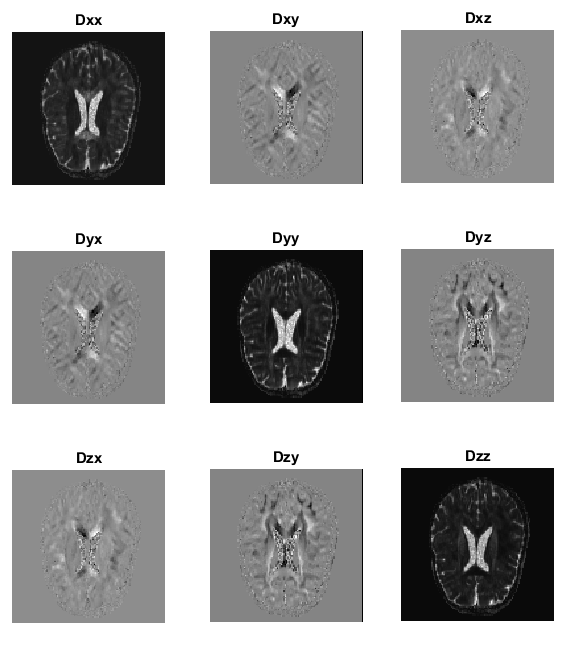
\includegraphics[width=16cm]{figures/Module_06/tensor_image}
	\centering
	\caption{Diffusion tensor estimate using the WLS-ABS method for a 126x126x55 test image.}
	\label{fig:m6_pic_2}
\end{figure}

We can then compute the eigenvalue decomposition of $\boldsymbol{D}$ and obtain eigenvalues and eigenvectors for each pixel of input image. Eigenvalues are sorted in descending order and saved for later computation (Fig.\ref{fig:m6_pic_3}). Moreover, eigenvectors corresponding to the highest eigenvalue are saved to separate variable, since they represent the direction of principal diffusion.

\begin{figure}[H]
	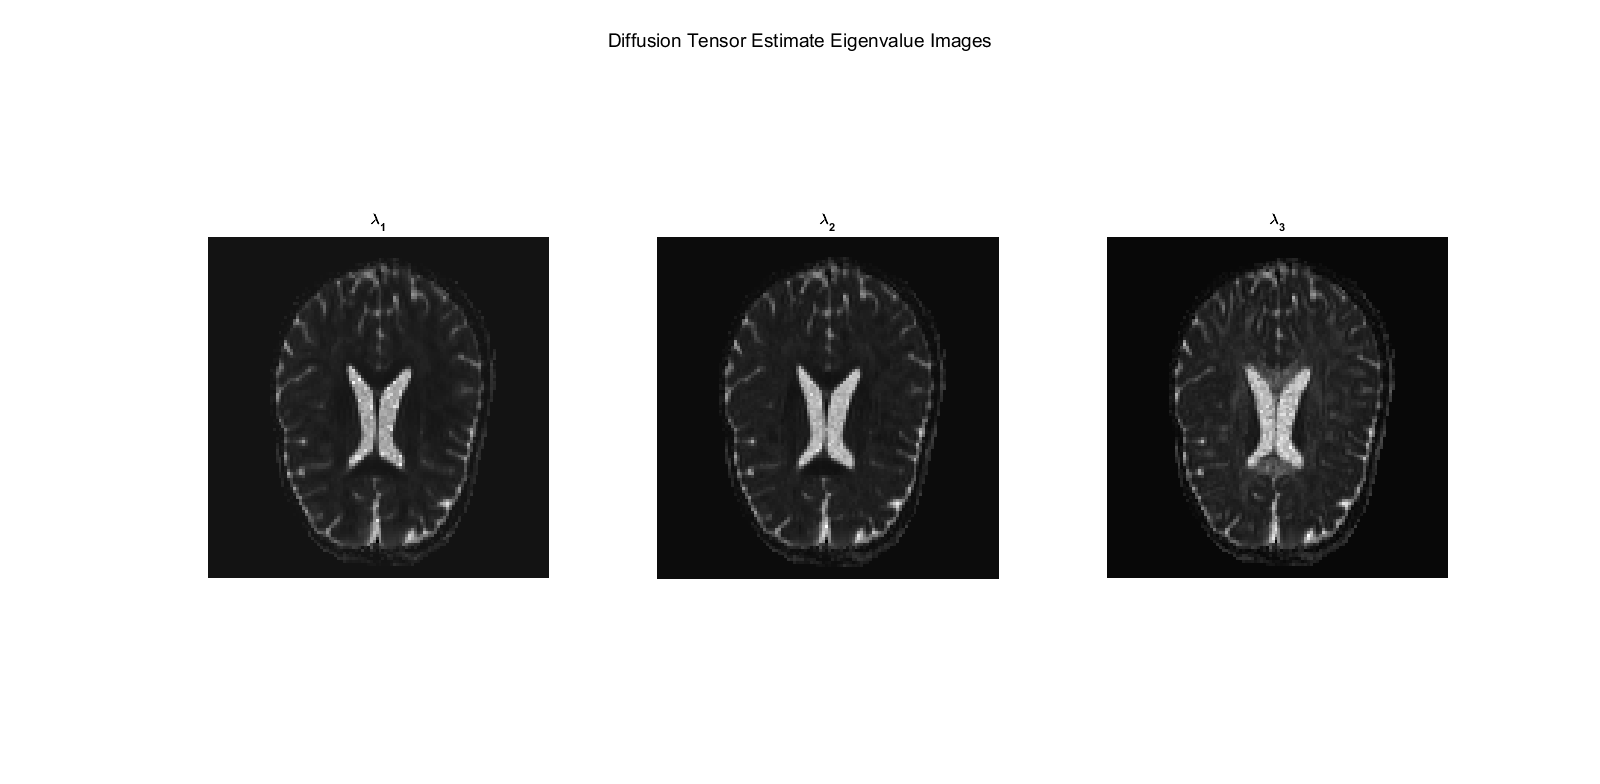
\includegraphics[width=16cm]{figures/Module_06/eig_image}
	\centering
	\caption{Diffusion tensor estimate eigenvalues of sample imgae; eigenvalues sorted in descending order from left to right.}
	\label{fig:m6_pic_3}
\end{figure}

Biomarkers are then computed using the following formulas:
\begin{equation}
MD = \dfrac{\lambda_{1}+\lambda_{2}+\lambda_{3}}{3}
\end{equation}
\begin{equation}
RA = \sqrt{\dfrac{\left(\lambda_{1}-MD\right)^2+\left(\lambda_{2}-MD\right)^2+\left(\lambda_{3}-MD\right)^2}{3\,MD}}
\end{equation}
\begin{equation}
FA = \sqrt{\dfrac{3}{2}}\sqrt{\dfrac{\left(\lambda_{1}-MD\right)^2+\left(\lambda_{2}-MD\right)^2+\left(\lambda_{3}-MD\right)^2}{\lambda_{1}^2+\lambda_{2}^2+\lambda_{3}^2}}
\end{equation}
\begin{equation}
VR = \frac{\lambda_{1}\lambda_{2}\lambda_{3}}{MD\,^3}
\end{equation}

Computed biomarkers of the sample image are presented on Fig.\ref{fig:m6_pic_4}. It is important to note that skull is visible because the brain area was selected by hand instead of relying on Module 08 output.

\begin{figure}[H]
	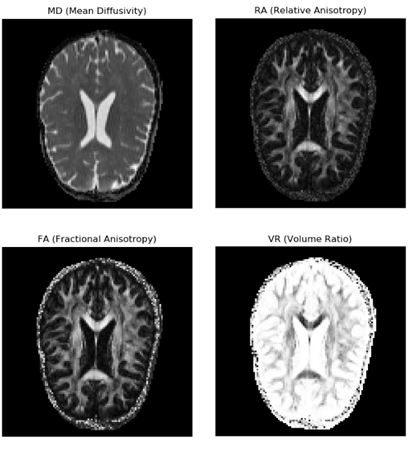
\includegraphics[width=12cm]{figures/Module_06/biomarkers_wls}
	\centering
	\caption{Diffusion biomarkers of sample image. Top left: MD, top right: RA, bottom left: FA, bottom right: VR.}
	\label{fig:m6_pic_4}
\end{figure}

Figure \ref{fig:m6_pic_5} presents the fifth biomarker image present in output dictionary - FA-weighted principal direction of diffusion color map. Color-encoded direction for this slice is presented as follows:
\begin{itemize}
	\item 
	red - transversal (left-right)
	
	\item 
	green - anterior-posterior (front-back)
	
	\item
	blue - cranio-caudal (head-feet)
\end{itemize}

\begin{figure}[H]
	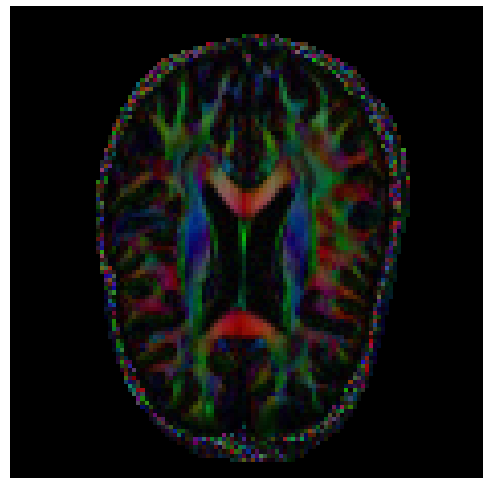
\includegraphics[width=10cm]{figures/Module_06/fa_rgb}
	\centering
	\caption{FA-weighted principal direction of diffusion of sample image.}
	\label{fig:m6_pic_5}
\end{figure}

\subsection{Implementation caveats}

Module source code was implemented and tested on a single sample image outlined above. It constituted a perfect basis for algorithm evaluation because it was already preprocessed, without the need to wait for other modules implementation. Even though it lacked a skull stripping mask, hand-drawn shape was good enough for testing, even though skull outline is visibly present, particularily on Fig.\ref{fig:m6_pic_5}. 

It was difficult to determine which estimation method - WLS or NLS - is objectively better. WLS was significantly faster and it was not much different from NLS results. This might have been due to the fact, that the diffusion-encoding gradient matrix was unusually large (7 structural images and 48 DWIs). Testing on preprocessed raw data, supplied for application evaluation has shown differences between methods, although both estimates are valid (to the Author's best knowledge) as it is difficult to compare any estimation methods without reference.

Initially developed using nested for-loops, DTI module has been vectorized to speed up computations. For a supplied 256x256x16 DWI stack a single slice is being processed in less than 3 seconds for WLS-ABS, while other methods scale linearily with chosen number of iterations (starting at 6 seconds, then 3 seconds per MFN iteration). It must be noted that the module was not tested with skull stripping mask, which could have drastically reduced computation time. Moreover computation time heavily depends on hardware constraints.

\section{Module 8. Skull stripping}

Preliminary processing to isolate the brain form extra-cranial or non-brain tissues such as e.g. the eye sockets, skin from MRI head scans is commonly referred as skull stripping. Skull stripping methods which are available in the literature are broadly classified into five categories: mathematical morphology-based metods, intensity-based methods, deformable surface-based methods, atlas-based methods, and hybrid methods. Each skull stripping method has their own merits and limitations.
The aim of this module is to remove pieces of skull from MRI Image using at pleasure chosen algorithm from the literature. Skull stripping is performed with use of two methods:
\begin{itemize}
    \item {Brain Surface Extractor BSE proposed by Stattuck et al. [1]}
    \item {Marker-controlled watershed algorithm by Abdallah and Hassan and by Segonne et al. [2], [3]}
\end{itemize}
Before this methods, there is applying preprocessing function to estimate global parameters: CSF - an upper bound for the intensity of the cerebrospinal fluid, COG - the coordinates of the centroid of the brain, BR - the average brain radius and ratio to brain diameter in axis x to brain radius in axis y. These estimated parameters are useful in this to methods to optimization and working.
BSE procedure consist of three steps:
\begin{enumerate}
\item {The MRI is processed with anisotropic diffusion filter to smooth nonessential gradients.}
\item {The filtered image has applied a Marr-Hildreth edge detector to identify important anatomical boundaries.}
\item {Using a sequence of morphological and connect component operation to define object by previous boundaries.}
\end{enumerate}

Anisotropic Diffusion filtering is applied to smooth noisy regions, which can obscure boundaries or their edges can be indistinguishable from the other in the image. To implement this filter is used an image processing method by Perona and Malik. They demonstrated that using the gradient of image intensity as an estimate of edge strength produces good results. The filtered image is modeled as the solution to the anisotropic diffusion equation
\begin{equation}
    \frac{\partial I}{\partial t} = \nabla \cdot (c(\textbf{p},t)\nabla I) = c(\textbf{p},t)\nabla^{2}I + \nabla c \cdot \nabla I  \label{Eq:wzor_1}
\end{equation}
where \textbf{p} is a point in $R^{2}$, $\nabla$ and $\nabla^{2}$  represent the gradient and Laplacian operators and $\nabla$ $\cdot$ indicates the divergence operator. The function is defined as:
\begin{equation}
    c(\textbf{p},t) = g(\parallel\nabla I(\boldsymbol{p},t)\parallel) = e^{-\parallel\nabla I(\textbf{p},t)\parallel^{2} \kappa^{2}_{d}} \label{Eq:wzor_2}
\end{equation}
where $\kappa_{d}$ is the diffusion constant. \eqref{Eq:wzor_2} gives preferences to high-contrast edges. Number of iteration and the diffusion parameter $\kappa_{d}$ is selected empirically.

To locate the anatomical boundaries in MRI brain volumes, it is used the Marr-Hildreth edge detectors. It is based on a low-pass filtering step with a symetric Gaussian kernel, followed by the localization of zero-crossing in the Laplacian of the filtered image. The Marr-Hildreth operator is defined as:
\begin{equation}
    C(k) = \nabla^{2}(I(k)*g_{\sigma}(\textbf{p})) \label{Eq:wzor_3}
\end{equation}
where C is the output contour image, I is an input image, * is the convolution operator, $g_{\sigma}$ is a Gaussian kernel with variance $\sigma^{2}$
\begin{equation}
    g_{\sigma} = \frac{1}{\sqrt{2\pi}\sigma}e^{- \parallel\textbf{p}\parallel^{2}/2\sigma^{2}} \label{Eq:wzor_4}
\end{equation}
where \textbf{p} is a point in the image, and $\nabla^{2}$ is the Laplacian operator.
To find pixels in the contour image, C where zerocrossing occur, a binary image E is produced that separates the image into edge-differentiated segments. Small values for sigma produce narrow filters, resulting in more edges in the image, on the other hand increasing this value makes the blurring kernel wider and only strong edges remain. This detector output is an image, which edge pixels are black and nonedge ones are white.

Morphological processing’s task is to select the pixels corresponding to the brain tissue from the original image. The output of edge detector often does not distinguish meninges or blood vessels from the brain tissue due to noise, low contrast between brain and meninges or true anatomical continuity. The first step is morphological erosion, which delete narrow connections without globally damaging image. After that the largest connected region centered in the volume consist entirely of brain tissue. Second step is selection of this region. Third step, is binary dilatation to restore the brain due to previous erosion, which decrease brain surface. Because of imperfections in the edge boundaries detection, image after dilatation may consist of pits in its surface or small holes within the surface. The last step of morphological processing is closing, which fill small pits and close of some holes that occur.

Marker-controlled watershed segmentation follows this procedure:
\begin{enumerate}
    \item {Computation a segmentation function.}
    \item {Computation the foreground markers.}
    \item {Computation the background markers.}
    \item {Computation of the watershed transform using of the foreground markers and the background markers.}
\end{enumerate}
First step is applied to find the edges in the image, it is processed with Sobel edge filter. The gradient is high at the borders of the object and low inside. Morphological techniques are used to compute the foreground markers, opening by reconstruction and closing by reconstruction to clean up the image. These operation will create flat regional maxima inside each object that can be used to find regional maxima and next modified them by a closing followed by an erosion to obtain good foreground markers. The background pixels after binarization are black, but their markers should be to close to the edges of the object. this can by done by computing the watershed transform of the distance transform of the binary image and the looking for the watershed ridges lines of the result. With the foreground markers and the background markers there is applied watershed based segmentation.

Brain Surface Extraction and Marker-controlled Watershed Segmentation is working separately. The base method is BSE. Marker-controlled watershed segmentation is compute, when BSE brain mask is larger than a mask based on preprocessing estimated BR.

\hfill{}\\
\textbf{List of References}\\
\cite{8_dti_1}, \cite{8_dti_2}, \cite{8_dti_3}, \cite{8_dti_4},


\section{Module 9. Segmentation}

Brain MRI segmentation is an essential task in many clinical applications
because it influences the entire analysis. This is because different
processing steps rely on accurate segmentation of anatomical regions.
For example, MRI segmentation is commonly used for measuring and visualizing
different brain structures, for delineating lesions, for analysing
brain development, and for image-guided interventions and surgical
planning.

\textit{MRI Processing} To prepare brain MRI for segmentation, it
is necessary to perform several preprocessing steps. (Fig. \ref{fig:Preprocessing}).

\begin{figure}[H]
\centering{}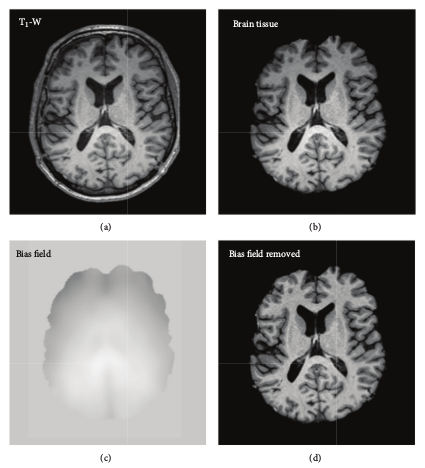
\includegraphics[scale=0.7,bb = 0 0 200 100, draft, type=eps]{9Preprocessing}\caption{Triangulation for the 15 patterns. \label{fig:Preprocessing}}
\end{figure}

The most important steps are: MRI bias field correction, image registration
and brain extraction.

\textit{Basic} An image for segmentation can be defined in 2D space
(pixels) or in 3D space (voxels). Each image element is specified
by its intensity value and coordinates for pixels (i,j) and for voxels
(i,j,k). Intensity values are typically represented by a gray value
{0, …, 255}.

The goal of image segmentation is to divide an image into a set of
semantically meaningful, homogeneous, and nonoverlapping regions of
similar attributes such as intensity, depth, color, or texture. Thesegmentation
result is either an image of labels identifying each homogeneous region
or a set of contours which describe the region boundaries.

Fundamental components of structural brain MRI analysis include the
classification of MRI data into specific tissue types and the identification
and description of specific anatomical structures. The problems of
segmentation and classification are interlinked because segmentation
implies a classification, while a classifier implicitly segments an
image. In the case of brain MRI, image elements are typically classified
into three main tissue types: white matter (WM), gray matter (GM),
and cerebrospinal fluid (CSF) (Fig. \ref{fig:Segment}).

\begin{figure}[H]
\centering{}\includegraphics[scale=0.7,bb = 0 0 200 100, draft, type=eps]{9Segmentation}\caption{Triangulation for the 15 patterns. \label{fig:Segment}}
\end{figure}

One of the most important features for brain MRI segmentation is the
intensity of brain tissue. However, intensity-based segmentation algorithms
will lead to wrong results when intensity value are corrupted by MRI
artifacts.

\textit{MRI Segmentation Methods} There is no single method that can
be suitable for all images, nor are all methods equally good for a
particular type of image. For example, some of the methods use only
the gray level histogram, while some integrate spatial image information
to be robust for noisy environments. Some methods use probabilistic
or fuzzy set theoretic approaches, while some additionally integrate
prior knowledge (specific image formation model, e.g., MRI brain atlas)
to further improve segmentation performance. The segmentation methods,
with application to brain MRI, may be grouped as follows: 
\begin{itemize}
\item manual segmentation; 
\item intensity-based methods (including thresholding, region growing, classification,
and clustering); 
\item atlas-based methods; 
\item surface-based methods (including active contours and surfaces, and
multiphase active contours); 
\item hybrid segmentation methods. 
\end{itemize}
\hfill{}\\
\textbf{List of References}\\
\cite{09a1}

\section{Module 10. Upsampling}

The implementation began with making a decision about the input data. The input image has to be 2 dimensional without a noise. The uploaded image will be considered as a 2 dimensional array of double values. Other parameters that will be needed are vertical and horizontal extensions. It has to be a total number. The size of the input array will be multiplied by the number. For example, the image 256x256 pixels with extensions equal to 3 will be 768x768 pixels as an output. The function needs also the window size. In one iteration, the function will take into consideration only pixels witch are inside the window. The loop will stop only when the whole image will be interpolated. To see the results the \textit{plotting} parameter has to be a boolean \textit{True} value. 
\newline The below picture shows the block diagram of the algorithm (Fig. \ref{fig: Module10_4}) with comments added.

\begin{figure}[H]
\centering{}\includegraphics[scale=0.7]{figures/Module_10/Module10_4}\caption{Algorithm block diagram with comments}. 
\label{fig: Module10_4}
\end{figure}

The following steps of the implementation will be discussed:

\begin{enumerate}

\item \textbf{Initial interpolation}
\newline To form the input image into the output with chosen size the initial interpolation is needed. As showed in \cite{9art1} the spline interpolation is used. In short, spline interpolation is an interpolation where interpolant is a special kind of piecewise polynomial called spline. It is recommended, because of the fact that the method makes small error even with low degree polynomials for the spline. Taking into consideration the edges the extrapolation was applied. To be more specific, the last row \textit{n} is equal to the previous one \textit{n-1}. The same with the first row, the first column and the last column of the input. To show the results, the extensions are set as 2. The input data is 256x256 pixels. The undermentioned picture (Fig. \ref{fig: Module10_5}) shows the result of the initial interpolation. The scale is included so it is easy to see that the size is twice as big. Now, the zeros (Fig. \ref{fig: Module9_3}) have  nonzero values, so the next steps can be made.


\begin{figure}[H]
\centering{}\includegraphics[scale=0.5]{figures/Module_10/Module10_5}\caption{The image after initial interpolation 512x512 pixels}. 
\label{fig: Module10_5}
\end{figure}

\item \textbf{Regularization}
\newline The main functionality is the regularization step. The function makes the square window which contains some pixels. In one iteration of a loop, only the pixels which are inside the window are considered. Next, the window moves and takes another pixels. It is repeated till the end of the image. The main goal is to determine of the weight which will be used at the end.
\newline The first weight is calculated as the difference between the pixels intensities.
\newline 
\centerline {$w_{1}(x, y)= e^{\frac{|N(x)-N(y)|^{2}}{h^{2}}}$, where}
\newline
\newline $N(x)$, $N(y)$ are window and image intensity values,
\newline $h$ is a level, which is equal to the half of the standard deviation of the input image.
\newline The next part of the whole weight is an Euclidean distance weight. It is simply calculated as the Euclidean distance between every pixel in the window and every pixel in the image. It is based on the below equation.
\newline
\centerline{ $w_{2}(x,y)=\frac{\sqrt{(x_{1}-x_{2})^{2}+(y_{1}-y_{2})^{2}}}{h^{2}}$, where }
\newline
\newline $h$ is a level, which is equal to the half of the standard deviation of the input image.
\newline The total weight is calculated as $w_{total}=w_{1}*w_{2}$. The output image is determined as the result of the sum of the multiplication of the weight and the window, divided by the sum of the weight.

\item \textbf{Mean correction}
\newline The mean correction step is a place in the function where the correctness of the equation $X=X+NN*(D(X)-y)$. It was abovementioned, that the downsampled HR has to be equal to the input data.

\item \textbf{Tolerance checking}
At the beginning it was established that only the 2D images will be taken into consideration and the upsampling function will be applied only once, so the step is excluded. There were experiments to upsample the data several times, but the result were not satisfied.

\end{enumerate}


\section{Module 11. Brain 3D}

\indent The implementation of 11th module includes visualization of cortex structure in three-dimensional model and visualization of elected cross-section of model. \\
\indent  As input parameter, module gets ouput of 9th module. This is the mask of segmentated data, which includes cortex structure as value 3. The data about cortex structure is seperated from 3D array.
11 th module is displayed in new window of application, so implementation includes not only functionality requirements but also design of graphical user interface.  \\
\indent To prepare design of user interface used Qt Designer program. \\
\indent Module is selected by user in main window of application. If input data is correct, new window is opened and reconstrucion of three-dimensional model is initialized automatically. \\
\indent First input data – 3D array – is converted to vtkFloatArray, which makes vtkImageData object. Then basing on vtkImageData there is used vtkMarcingCubes class, which makes reconstruction. As a threshold there is used value equal to 1, because of fact that all values not equal to zero are included to cortex structure. \\
\indent After reconstrucion model is displayed in BRAIN 3D window. To enable displaying VTK objects in Qt Application there is set frame in which is inserted the object of VTK library by using QVTKRenderWindowInteractor. It is dedicated vtkWidget to display VTK in QT ibrary.\\
\indent To visualization data there are used following classes:
\begin{itemize}
\item vtkRenderer – which enables rendering process: transforming geometry, light and camera view into an image
\item 
vtkMapper – which maps data to graphics primitives
\item vtkActor – adjusting data to 3D scenery
\item vtkInteractorStyleTrackballCamera – setting possibility of interaction with model
\end{itemize}
\indent BRAIN 3D window enables three options:
\begin{itemize}
\item preview 3D model
\item clip model 
\item clip model and show plane.
\end{itemize}
\indent Automatically after initialization there is loaded firts mode: preview 3D model. 
Mode: clip model, enables to set intersection plane and cut model in place of it. Intersection plane is vtkImagePlaneWidget object. It allows to interactive set the plane by computer mouse. Interaction of plane is activated whenever user presses „clip model” button. When interaction event is detected the model is automatically clipped by vtkCliPolyData class. \\
\indent Mode:  clip model and show plane calls the same function as previous mode, but with input parameter planemode - True ( default – False). It expands functionality of diplaying the cross-section corresponding to the elected plane. It improves readability of intersection plane. It is based on the same objects of VTK library, but using additional methods of it.\\
\indent User has possibility fluently switch modeLs by pressing appropriate buttons. Application has also help window, with short user guide.


\section{Module 12. Oblique imaging}

\indent The literature to this module is as useful as nipples on
men. Everything is about inventing how to realize point 1. of the
list. \\
 \indent Oblique Imaging is a technique to create non-perspective
projections from 3D or multiple 2D images.\\

\indent In order to create oblique image it is essential to: 
\begin{itemize}
\item choose two angles under which the plane will be inclined, 
\item create a matrix of points that this plane consists of, 
\item from existing points pick those, which will be used in the image, 
\item interpolate points that are not existing. 
\end{itemize}
\indent Type of interpolation can vary, but in this project interpolation
based on mean will be used. To interpolate one pixel mean of all pixels
around him with given proximity is taken.

\begin{figure}[H]
\centering{}\includegraphics[scale=0.7]{figures/m11_spherexyz}\caption{Visualization of pixels taken to interpolate}
\label{fig:figures/m11_spherexyz } 
\end{figure}

\input{"Tests/Application"}


\chapter{Authors}

Authors of this project are students of Biomedical Engineering, AGH
UST, Krakow, Poland. \\

\begin{center}
\begin{tabular}{|c|c|}
\hline 
Name  & Role \tabularnewline
\hline 
\hline 
Sylwia Mól  & Project Manager\tabularnewline
\hline 
Jacek Fidos  & Software architect\tabularnewline
\hline 
Maciej Gryczan  & GUI engineer\tabularnewline
\hline 
Adrian Stopiak  & Vizualization engineer \tabularnewline
\hline 
Malwina Molendowska  & 1st module developer \tabularnewline
\hline 
Klaudia Gugulska  & 2nd module developer \tabularnewline
\hline 
Kacper Turek  & 3rd module developer \tabularnewline
\hline 
Magdalena Rychlik  & 4th module developer \tabularnewline
\hline 
Alicja Martinek  & 5th module developer \tabularnewline
\hline 
Mateusz Pabian  & 6th module developer \tabularnewline
\hline 
Anna Grzywa  & 8th module developer \tabularnewline
\hline 
Magdalena Kucharska  & 9th module developer \tabularnewline
\hline 
Eliza Kowalczyk  & 10th module developer \tabularnewline
\hline 
Karolina Gajewska  & 11th module developer \tabularnewline
\hline 
Michał Kotarba  & 12th module developer \tabularnewline
\hline 
\end{tabular}
\par\end{center}

\newpage{}

\listoffigures

\printbibliography

\begin{comment}
 \bibliographystyle{plain}
\bibliography{bibliografia}
\end{comment}

\end{document}

